\pdfoutput=1 % only if pdf/png/jpg images are used
\documentclass{JINST}
\let\ifpdf\relax% Esto lo agrego por el warning que me tira al compilar por \ifpdf
\hyphenation{tem-pe-ra-tu-re}
\usepackage[utf8]{inputenc}
\usepackage[T1]{fontenc}
\usepackage{multirow}
\bibliographystyle{JHEP}

\title{The Latin American Giant Observatory: a Very Long Baseline Array of Ground Based Astroparticles Detectors}

\author{
	The LAGO Collaboration\thanks{Corresponding author.}\\
	web: \href{http://lagoproject.org}{lagoproject.org}\\
	email: \email{lago-pi@lagoproject.org}
}

\abstract{
The LAGO (Latin American Giant Observatory) project, aims at the detection of the
highest energy component of Gamma Ray Bursts. It consists in a wide network of
water Cherenkov detectors (WCDs) located at several sites in eight Latin
American countries. Recently it has been shown that WCDs can be used to study
the solar modulation of galactic cosmic rays and other transient effects, by
measuring the variations of the flux of secondary particles at ground level.
Long-term modulation and transient events can be characterized by using the
LAGO detection network, as it spans over a big area with different sites at
different latitudes, longitudes and geomagnetic rigidity cut-offs. In this work
the Observatory is presented with all its sites, and also the
capabilities to complement measurements of solar activity from ground level are
described. 

}
\keywords{Space Weather, Gamma Ray Bursts, Water Cherenkov Detector}

\begin{document}
\section{Introduction}\label{sec:intro}

Empezamos hablando de los RC en gral

para luego hablar un poquito de observaciones en tierra

y ahi entramos con LAGO


Gamma-ray bursts (GRBs) are the most powerful explosions known in the Universe.
They are sudden emissions of gamma-rays lasting very short time intervals (from
0.1 up to 500 seconds). They were discovered in 1967 by the Vela satellites
that the US government launched to monitor covert nuclear tests from space. In
1997 the BeppoSAX satellite detected an optical afterglow of a GRB.  When it
was analyzed it showed that the redshift of the galaxy that originated the GRB
was at more than 6 billon light years from Earth. This showed GRBs to be
extragalactic events. The astrophysical sources of these events are still
unclear but good candidates are the coalescence of compacts objects for the
short bursts (less than 2 s), and hypernovae, supernovae produced by very
massive stars, for the long bursts (more than 2 s) \cite{Meszaros2006}.

Despite satellites observations like SWIFT, FERMI and others, revealing
some questions about the origin and location of GRBs, other questions remain
unanswered, especially in the high energy region, i.e. the spectrum. Up to now
no ground-based experiment has detected a GRB.

The idea is that when high energy photons from GRBs reach the atmosphere, they
produce cascades that can be detectable at ground level by using WCDs. Instead
of trying to detect this extensive air showers individually, LAGO makes use of the single
particle technique, that is to observe an excess in the counting rates of
secondary particles produced in EAS \cite{Vernetto2000}. The main advantage of
using WCDs compared to other instuments, is their higher sensitivity to
photons, which are 90\% of the secondary particles at ground level for high
energy primary photons.

Although the original plan comprised the detection of the high energy component
of GRBs, recently it has been shown that WCDs can also be used to study the
Solar Modulation (SM) of galactic cosmic rays and other transient effects, by
measuring the variations of the flux of secondary particles at ground level
\cite{PierreAugerCollaboration2011}

The main effect is produced by the solar magnetic field. When the Sun shows a
high activity (intense magnetic field), galactic cosmic rays are deflected,
resulting in a reduction of their flux on Earth. When magnetic fields are less
intense we have a higher flux. So, by measuring the flux of galactic cosmic
rays one can determine indirectly the solar activity. This allows, for
instance, the observation of the eleven year cycle of the sun and also
transient events known as Forbush decreases. These decreases are produced
when a Coronal Mass Ejection (CME) is originated in the Sun, resulting in a
huge mass of plasma sent through the interplanetary medium. Upon reaching
Earth, this plasma perturbs the near space and results in a modification in the
flux of galactic cosmic rays. A rapid diminution of their flux can be
observed (a few percent in a few hours). Then, once the CME leave the earth surroundings,
the galactic cosmic ray flux slowly comes back to its original value, on a time
scale of days.

The LAGO project is a recent collaboration that comes from the association of
Latin American astroparticle researchers. It started in 2005 and it was
designed to survey the high-energy component of GRBs. It is a network of
ground-based WCDs, located at mountain altitudes, above 4500 m.a.s.l., where
the flux of the primary gamma-rays is too low for effective detection by small
area satellite detectors. This collaboration was motivated by the experience of
the Pierre Auger Observatory, and the idea is to install WCD in 9 Latin
American countries: Argentina, Bolivia, Brasil, Colombia, Ecuador, Guatemala,
Mexico, Peru and Venezuela \cite{Allard2008,Allard2009b}. More than 75 people
integrate the LAGO community, keeping a close collaboration with researchers
from IN2P3 of France and INFN in Italy.

LAGO can be an optimal detection network to characterize the SM and transient
events, as it spans over a large area with sites at different heights, latitudes,
longitudes and geomagnetic rigidity cut offs.


\section{Science case}\label{sec:science}

%%Fig. \ref{fig:lago-fb}, shows the comparison between a neutron monitor
%%in Rome, and a single WCD of 1.8 m$^2$ in Bariloche \cite{Asorey2013b} measuring
%%a Forbush decrease in 2012. As can be seen the LAGO detector shows similar
%%relative variation as the other two measurements.
%%
%%explayarse mas sobre space wheather con lago
%%
%%\begin{figure}
%%\includegraphics[width=.9\textwidth]{images/icrc2013-1109-05.pdf}
%%\caption{A Forbush decrease event seen by a single LAGO detector. The
%%comparison between the WCD in Bariloche and a neutron monitor in Rome shows a very good agreement.}
%%\label{fig:lago-fb}
%%\end{figure}

%%%%%%%%%%%%%%%%%%<< aca empieza la parte de dasso >>%%%%%%%%%%%%%%%%%%%%%%%%%%%%%%%%%%%%%%%%

% Intro context (que problema y a quien le interesa).
The transport of energetic particles or cosmic rays (CRs, both solar and galactic origin) in the
interplanetary medium and in the terrestrial environment (magnetosphere and upper/middle/lower atmosphere)
is a major topic of interest for space weather, presenting several unsolved questions
\cite[e.g., ][]{Wibberenz98, Belov00, Smart09, Kudela13}.
% Large scaler and transients.
Different physical mechanisms modulate the transport of CRs in the heliosphere.
Generally, they can be divided into large scale processes (mainly related to the magnetic field configuration in the whole heliosphere) and transient phenomena.
The last ones are mainly produced by transient solar processes, such as Interplanetary Coronal Mass Ejections (ICMEs)
or interplanetary shocks \cite[e.g., ][]{Wibberenz98}.

% NMs as historically typical ground detectors of CRs
Since more than 50 decades, neutron monitors have been the usual ground detectors for recording indirect 
observations of the variability of primary CRs fluxes arriving Earth with energies of interest
for space physics \cite[e.g., ][]{Meyer55}.
These detectos have provided data and clues to better understand different physical mechanisms
occurring during the interplanetary transport of CRs,
such as the anticorrelation between the solar activity and the galactic CRs fluxes,
the solar rotation combined with plasma streams ejected from coronal holes producing 27 days recurring
intensity variations, and transient Forbush decrease events (Fds).
Forbush decreases are observed depressions of the CR flux at the Earth ground level, which can last from hours to weeks.
They are generally observed in connection with the presence of ICMEs in the vicinity of the Earth \cite[e.g., ][]{Cane00}.

% muon detectors 
Muon detectors and muon telescopes are newer ground observatories for similar, and a bit larger, ranges of energies than neutron monitors
that can record variability of CRs associated with space physics and space weather phenomena \cite[e.g., ][]{Munakata12}.

% Recent CWDs (Auger and LAGO)
Recently, water Cherenkov detectors (WCDs) have shown the capacity of observing the variability
of the flux of CRs related with space weather phenomena \cite{FALAugerscalers11, AugerCOLAGE12, ICRC-Auger, ICRC-LAGO}.
The Pierre Auger Observatory, located in Malarg\"ue, Argentina (69.3 o W, 35.3 o S, 1400 m a.s.l.), can observe the variability
of CRs during a Forbus decrease using a single particle technique,
which consists in recording low threshold rates (the so-called scaler mode)
with all the surface detectors of its array \cite{FALAugerscalers11}.

% Some details of scaler and histogram modes at PAO.
The scaler mode at the Pierre Auger Observatory can detect a high total count rate, coming from the large area of the surface detectors
(greater than 16,000 m$^2$), reaching a flux of secondary particles as high as $\sim 10^8$ counts per minute
with a median energy for primary particles of $\sim 90$ GeV \cite{AugerCOLAGE12}, providing a very low statistical uncertainty for this counting.
From a comparison with Neutron Monitors from the Observatory at Los Cerrillos (6NM64), Chile, located
$\sim 250$ km westward from Malarg\"ue, it was shown the excellent sensitivity also to the daily modulation of the scalers \cite{AugerCOLAGE12}.
Another mode of interest developed at the Pierre Auger Observatory is the 'histogram mode', in which
the number of secundary particles are counted from discrimination of the deposited energy.
Forbush decreased has been observed even at energies as larger as XXX [ICRC-Auger-China].

% LAGO mostro que puede observar Forbush ICRC-LAGO-Rio
{\bf [Esto se debe compatibilizar con la intro del paper]}
The LatinAmerican Giant Observatory (LAGO) is a non-centralized network composed by more than 30 institutions from nine Latin American countries.
It is an extended CR observatory formed by WCDs, that make observations of the temporal evolution of the radiation flux at ground level.
{\bf [Decir que la red (citar a la otra seccion) tiene/tendra detectores a lo largo de una banda de longitudes (entre tal y tal)
que recorre un gran rango de latitudes (cuantificar).]}

% what to do in this section. Caso Study.
As a simple example of the potentiality of LAGO, in this section we describe
the interplanetary manifestation of a solar ejection happened on March 2012,
and the LAGO observations of the associated Fd.

% Contar un poco la historia del sol a la tierra, las particulas observadas en ese periodo.
Several Coronal Mass Ejections were erupted from the NOAA-AR-11429 during March 2012.
Three of them were launched toward Earth and produced space weather effects in the terrestrial ambient.
In particular, the CME ejected at 00:15 UT of March 7 was the largest one and was associated
with a long duration X5.4 flare peaked at 00:24 UT, launched with velocities $\sim$ 2400 km s$^{-1}$ \cite{Liu13}.
Depending on the velocity and the magentic polarity of ICMEs arriving Earth, they can produce geomagnetic storm,
enhancing the activity of the ring current system in the terrestrial environment
with decay times of the order of several hours \cite{Dasso02}.
The arrival of this ICME with its driven shock to Earth occurred at 10:19 UT of March 8,
and produced a major geomagnetic storm with consequence on the index Dst,
which reached a significant negative value of Dst=-143 nT.
This ICME also had strong consequences on the Earth CRs arrival. Neutron monitors present significant decrease
of their countings, observing a clear Forbush decrease in time agreement with the arrival of the ICME,
in particular the South Pole Neutron Monitor observes a decrease of $\sim -15\%$ \cite{DiFino14}.
%* Produce un Forbush observado por varios NMs (citar paper de Di Fino). Cuantificar porcentaje.
% La fig 4 del paper de ISS [Di Fino et al., J. Space Weather Space Clim, 2014] muestra el Forbush para dif NMs. 
% En South Pole (SOPO) alcanza mas de 15%. 
% Hay paper de NMs para este dia? Sip, el paper de ISS muestra una figura del Fd obs por varios NMs.

% Decir que este Forbush fue observado en primarias por PAMELA [citar a COSPAR poster] ?

% Contar que LAGO observo el Forbush.
% Comparacion con NM de Roma.
% (Hay que mencionar algun acknowledgment por mostrar resultados de Roma?).
Figure xxx shows this Forbush decrease observed by a single WCD of LAGO in Bariloche with a surface of 1.8 m$^2$, Argentina.
It can be osberved that this LAGO detector observed a FD peak of almost $\sim - 6\%$ at a place with a rigidity cutoff of XXX.
For a comparison, this figure also shows observations from the Neutron Monitor in Rome [cita?, agradecimientos?], where can be
seen the very good agreement between LAGO and Rome observations.

{\bf [Se sabe que hubo otra ICME que llego a la Tierra aprox mediodia del 12 de Marzo, con la ICME llegando hacia el final del 12/mar.
En Roma se ve un segundo Forbush montado antes que termine el primer. Pero parece que en LAGO hay un gap justo alli. Decimos algo del 2do evento?.
Tambien se ve que el final del Forbush ocurre aprox 23 marzo. Decimos algo sobre donde estan las ICMEs ese dia o se hace muy largo?
Creo que hay un paper que menciona algo de esto.]}
% * Mas alla de la Tierra?  Liu Apj 2014.

{\bf [Esto podria repetirse, reescribiendolo, en las conclusiones del paper]}
One of the major advantages of LAGO is its extension in geographical latitude (from equatorial latitudes up to the antartic region) and
altitudes (from sea level up to more than 5000 meters over sea level). Thus, the net covers a huge range of geomagnetic rigidity cut-offs
and atmospheric absorption/reaction levels.
From combining different ground sites, observations from the LAGO network, will make possible studies of the heliospheric modulation of galactic cosmic rays,
in particular will allow to study long-term modulation as well as transient events.


\section{Detector design}\label{sec:detector}


\subsection{Water Cherenkov Detector}

Thanks to its low cost, robustness, reliability and reasonable efficiency, on the of the most commonly used particle detectors in Astroparticle physics are the Water Cherenkov Detectors, with typical detection masses from one to thousands tons of water. The passage of ultra-relativistic charged particles through the water volume produce Cherenkov radiation mainly in 


that is collected by a central photomultiplier tube (PMT), typically an
8-inch Hamamatsu R5912 PMT. The sensitivity to secondary gammas in the cascade
is enabled by the production of Cherenkov capable electron/positron pairs




Based on the geographical distribution of the sites where LAGO operates, the basic design principles for LAGO detectors are simple: we focus on the utilization of low cost and low power consumption off the shelf components. The LAGO smart WCD are built starting from commercial polyethylene water tanks with $\sim 1$\,m$^3$ to $40$\,m$^3$ of purified water. 




The passage of
ultra-relativistic charged particles through the water volume produce Cherenkov
light that is collected by a central photomultiplier tube (PMT), typically an
8-inch Hamamatsu R5912 PMT. The sensitivity to secondary gammas in the cascade
is enabled by the production of Cherenkov capable electron/positron pairs
within the water volume. The detector has an internal coating made by a highly
diffusive and reflective fabric of commercial
Tyvek\textregistered
%\footnote{http://bit.ly/1whxoph}
. The diffusion of
Cherenkov photons in the fabric surface reduce the signal dependence with the
secondary particle trajectory within the detector. A FPGA based, own designed
fast analog-to-digital conversion electronics allows the operation of up to
four independent detectors in a same site. This electronics is controlled by a
Raspberry Pi or similar device. Additionally, the station has a temperature and
atmospheric pressure sensor and a GPS board for time synchronization between
different LAGO sites. The power consumption of the station is less than $11$\,W
and is powered by solar panels and batteries. The LAGO WCD are characterized by
its low cost and reliability, and a schema of this detectors can be seen in
figure \ref{lago_wcd}.





Estos dispositivos detectan la
radiación Cherenkov producida por el paso de una partícula cargada con
velocidad mayor a la velocidad de la luz en el agua. Otra de las ventajas de
los WCD es su capacidad para detectar los fotones presentes de las
cascadas\,\cite{Allard2007,AllardEtal2008, AllekotteEtal2008}, que constituyen
el $\sim 70\%$ del total de partículas de la EAS. Con un metro cúbico de agua
se alcanzan altas probabilidades de conversión de un fotón en un par
$e^\pm$\,\cite{Asorey2012b}. En la figura\,\ref{WCDEsquema} se muestra un
esquema del detector típico utilizado en el proyecto LAGO. Alrededor del mundo
existen varias instalaciones de WCD dedicadas a la detección de GRB: INCA en
Chacaltaya-Bolivia $5200$\,m s.n.m.\,\cite{Cabrera1999}; Milagro en Nuevo
México-EE.UU. a $2650$\,m s.n.m.\,\cite{Atkins2004}; el Observatorio Pierre
Auger en Malarg\"ue-Argentina a $1400$\,m s.n.m.\,\cite{Abraham2004a}, y HAWC
en Sierra Negra-México, a $4500$\,m s.n.m\,\cite{Abeysekara2012}.

Los WCD del proyecto LAGO pueden tener variadas geometrías, y un esquema típico
se muestra en la figura \ref{WCDEsquema}. En general están construidos a partir
de un tanque comercial para almacenamiento de agua, con una capacidad de entre
$1$\,m$^{3}$ y $10$\,m$^{3}$, llenos de agua purificada. Cada WCD de LAGO
replica la idea de los WCD del Observatorio Pierre Auger de manera simplificada
y económica. La independencia en la detección de señales respecto a la
dirección de movimiento de las partículas se logra al tapizar internamente el
detector con Tyvek, un material altamente reflexivo y difusivo, que logra la
uniformización de la radiación Cherenkov en tiempos del órden de $15$\,ns luego
del ingreso de la partículas al detector\,\cite{Asorey2012b}. Las señales
luminosas son convertidas en señales eléctricas mediante un PMT de alta
sensibilidad, alta ganancia y alta linealidad. Las señales provenientes del PMT
son digitalizadas mediante una electrónica de diseño propio de la colaboración
LAGO. Estas placas utilizan conversores analógico-digitales rápidos (FADC, por
sus siglas en inglés, \textit{Fast ``flash'' analog-to-digital converters}) con
una velocidad de muestreo de $40$\,MHz y con una resolución de $10$\,bits. Las
placas permiten además controlar las tensiones de polarización del PMT, y
disponen de tres canales independientes de digitalización y control. Se utiliza
una FPGA (\textit{Field Programmable Gate Array}) Digilent Nexys-II para el
control del GPS, del sensor de Presión y Temperatura y de la electrónica de
adquisición. Las señales digitales son procesadas por la FPGA y transferidas a
una computadora por el puerto USB. Esto dificulta la adquisición en sitios
remotos por el alto consumo de la PC de adquisición, y es por ello que en esta
propuesta se estudia la implementación de dispositivos de bajo consumo para el
control y almacenamiento de datos (Raspberry Pi y dispositivos de
almacenamiento de estado sólido). Una descripción completa del funcionamiento
de los WCD y de grandes arreglos de detectores puede consultarse
en\,\cite{Asorey2012b}.

La técnica utilizada por la colaboración LAGO para detectar GRB y fenómenos
solares es conocida como la técnica de partícula individual
(SPT)\,\cite{Vernetto2000}. Esta técnica se fundamenta en la detección de una
elevación en la tasa de conteo sobre un fondo base, en escalas de tiempo
relacionadas con los fenómenos a observar (desde algunos segundos para GRB
hasta semanas para la recuperación del flujo de secundarios luego de un FD).
Estas variaciones en el flujo de secundarios pueden ser correlacionados con
variaciones en el flujo de primarios en el límite superior de la atmósfera.
Esta técnica ha sido utilizada con éxito para la detección de fenómenos solares
en el observatorio Auger\,\cite{ThePierreAugerCollaboration2011,Asorey2011a}.
La SPT es, hasta ahora uno de los pocos métodos para detectar GRB en el rango
de los GeV, y puede verse una descripción completa aplicada a LAGO por
\cite{BertouAllard2005}. La elevación de un conteo de base en $5 \sigma$
durante un segundo representa un aumento de $\approx 270$ partículas\,m$^{-2}$
y a $5300$\,m s.n.m. un fotón de 100 GeV produce $\approx 290$
partículas\,m${-2}$, con lo cual un fotón de esa energía podría ser detectado
con un WCD de sólo $1$\,m$^2$ de superficie\cite{BertouAllard2005}. Por ello la
colaboración LAGO apunta a colocar detectores en elevaciones, por cuanto
$10$\,m$^{2}$ de WCD en $5300$\,m s.n.m. tienen la misma sensibilidad para
búsqueda de GRB que toda la instalación del Observatorio Pierre Auger con
$16000$\,m$^{2}$ de superficie de
detección\,\cite{AllardEtal2009A,AllardEtal2009B}.

A más altas energías, la dispersión lateral de las partículas en las EAS hace
que puedan encontrarse partículas provenientes de una misma cascada, y por lo
tanto correlacionadas, a cientos de metros y hasta algunos kilómetros de la
dirección de propagación de la partícula primaria. Por lo tanto, al disponer de
un arreglo de detectores espacialmente separados y temporalmente sincronizados
es posible muestrear la distribución lateral de las partículas en la lluvia.
Esto permite buscar correlaciones espacio-temporales entre las señales de los
distintos detectores, lo cual a su vez posibilita la triangulación de las
señales y sus intensidades, y de esta manera reconstruir la dirección de arribo
y la energía del rayo cósmico incidente\,\cite{Asorey2005}. La sincronización
temporal requerida es de algunos nanosegundos entre detectores separados a
algunos kilómetros, lo cual puede lograrse de manera simple, económica y
eficiente usando receptores GPS comerciales funcionando en el modo
{\textit{pulso por segundo}}\,\cite{Pryke1995}.

\begin{figure}
  \begin{center}
    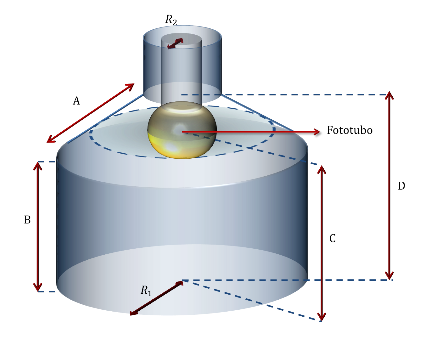
\includegraphics[width=0.4\textwidth]{images/detector.png}
    \caption{Esquema de un WCD típico de LAGO. El detector está formado por un
tanque plástico o metálico comercial de geometría cilíndrica o cilindro-cónica
y dimensiones variables, que contiene entre $1$\,m$^3$ y $10$\,m$^3$ de agua en
su interior. El pasaje de partículas cargadas ultra-relativistas por el agua
produce radiación Cherenkov en el interior del detector. Esta radiación es
reflejada y difundida gracias a un recubrimiento interno hecho de Tyvek. Luego,
un tubo fotomultiplicador de entre $6$\" y $9$\" capta la radiación Cherenkov y
la convierte en señales eléctricas, que luego son digitalizadas, procesadas y
almacenadas para su posterior análisis.} \label{WCDEsquema}
  \end{center}
\end{figure}

\subsection{Description of the data acquisition electronics}\label{sec:electronics}

A WCD is composed by a tank of water with a reflective material inside, and a
photomultiplier tube (PMT) to convert Cherenkov radiation produced by the
interaction of the high energy particles with water in an electric signal. The
response of each WCD, like other particle detectors, are short electric pulses
that are recorded by high speed data acquisition systems.

\subsubsection*{Bariloche design}

The PMT is connected to a electronic board, that have a voltage divider, a high
voltage supply, and an amplifier of the output pulse. The high voltage supply
can be controlled typically from 0\,V to 2000\,V with a signal from 0\,V to
5\,V. The output pulse shape of the PMT depends on the geometry of the tank,
for a tank of 1000\,l the FWMH (Full Width at Half Maximum) of the pulse is
around 150\,ns. At the same time, it is necessary to measure other information
relevant to the experiment, like pressure, temperature and PPS (Pulse Per
Second) from the GPS. The data acquisition and high voltage parameters of the
experiment can be settled by a PC program and the acquire pulses are transfered
in real time to the PC via a USB interface. This system has the capabality of
acquire three independent channels of pulses and provide the control signal for
the three HV supply.  Figure \ref{fig:electronic-b}, top, shows a block diagram
of the data acquisition system.

The data acquisition system includes a custom electronic board that integrate
the front-end electronics: three ADC, anti-aliasing filters, baseline control
control circuit, high voltage control signal, and the necessary service
circuits. This board is connected to a NEXYS-2 board \cite{nexys2} via a high
speed FX2-Hirose connector. The NEXYS2 have a FPGA Spartan3E that is connected
to the PC with a USB interface. The USB interface between the PC and the FPGA
is managed with a Cypress chip included in the board. In the FPGA there is an
implementation of a module of command, that provided connectivity with the
sensors the GPS and with a pre-processor that filter the input pulses. The
pulses that have an amplitude over a trigger level are transferred to the PC.
Every time that a PPS from the GPS occurs, the systems sends to the PC the
values of the preassure, temperature and the UTC time from the GPS. There is
also an implementation of a stabilizer circuit for the baseline.

A sub-trigger mode was specially developed for LAGO, it makes possible to
acquire only the amplitude and charge value of pulses that have amplitude above
a pre-seted value of ''sub-trigger''. With this feature is possible to  record
a high rate 100KHz of pulses without loss of data. This makes possible do a
classification in energy versus particle rate for the study of  solar physics
\cite{asorey:13}. For the proper operation of the sub-trigger mode, it is
necessary to get a stable baseline. A stabilizer circuit of the baseline is
implemented.

In figure \ref{fig:electronic-b}, bottom, a casing with the whole LAGO
electronic can be seen with the different components. The NEXYS-2 board with a
sensor for pression and temperature (HP03S), a switching power supply and a
digitalized board with three available channels.

\begin{figure}[htp!]
 \centering
 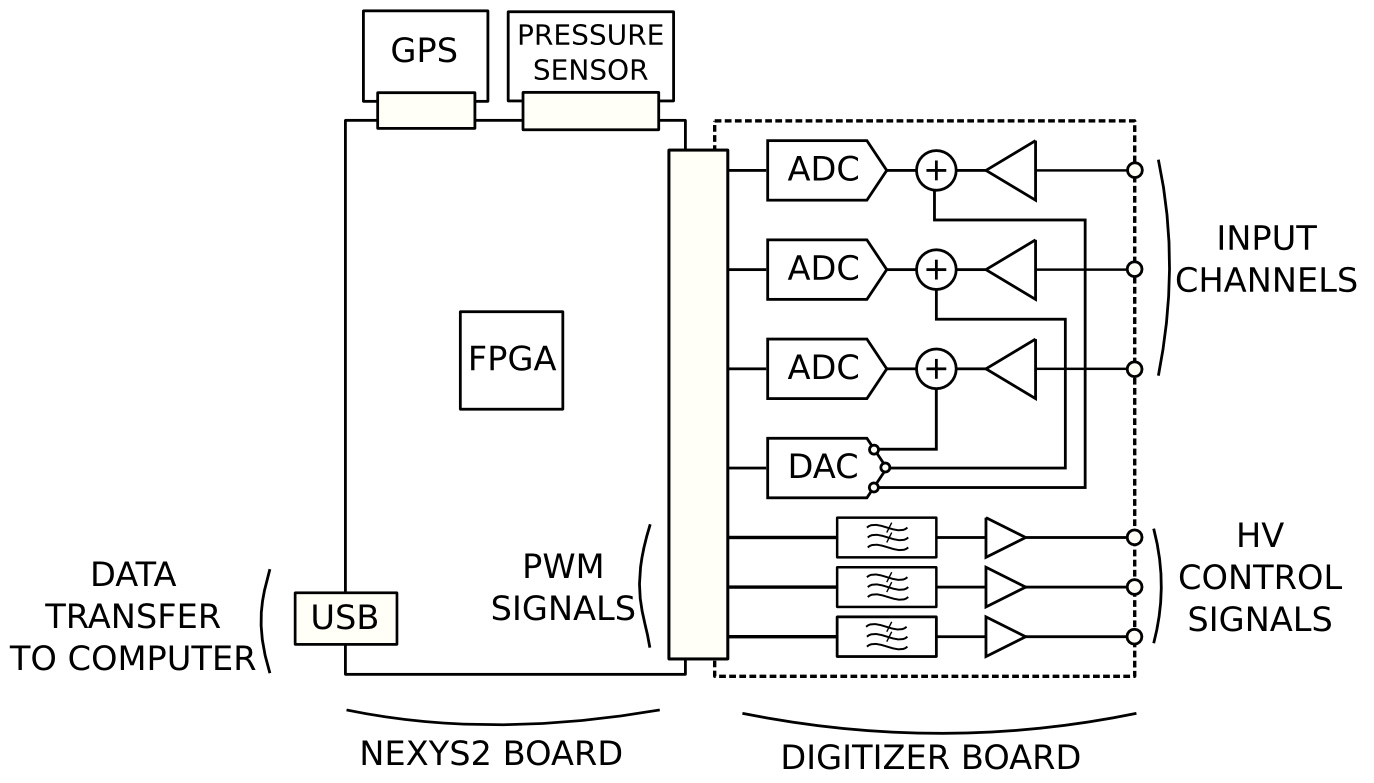
\includegraphics[width=0.65\textwidth,height=0.25\textheight]{images/bloques_electronica.png}
 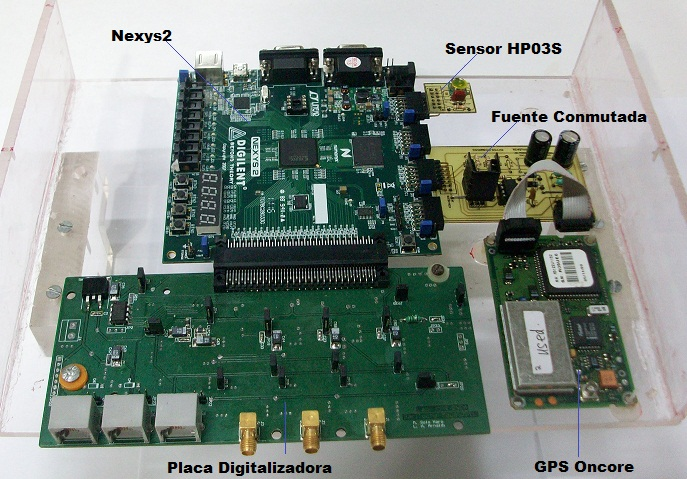
\includegraphics[width=0.70\textwidth,height=0.30\textheight]{images/venezuela/nuevaLS.jpg}
 \caption{Top: block diagram of the DAQ developed by LAGO Bariloche. Bottom:
Electronic kit designed for the LAGO collaboration, in the version assembled by
LAGO Venezuela} \label{fig:electronic-b}
\end{figure}  

\subsubsection*{Mexico design}

Field programmable gate arrays (FPGAs) was playing an increasing role in DAQ
systems in cosmic rays experiments due to their high speed and integration and
their low cost and low power consumption. Modern electronics based on on-chip
fast analog to digital converters (ADCs) and powerful digital signal processors
(DSPs) was being  ideal to be the basis of custom-made DAQ systems which are
more flexible, faster and cheaper than the traditional DAQ systems based on
modular electronics \cite{all:09}. We took advantage of these recent
developments, in particular in the area of very high integrated circuits in the
form of ADCs and FPGAs for the design of the new system which consisted of an
ADC daughter board running at 200 MSPS\footnote{Mega Samples Per Second}. Each
event was tagged with precise GPS time using a GPS embedded receiver with 1 PPS
(one pulse per second) synchronised with the atomic clock on the GPS satellites
within a corrected uncertainty of 50\,ns (Motorola Oncore UT+ module)\ref{ref}.
A pressure and Temperature sensor (HP03D) was adapted to the FPGA board (2FT
Xilinx).

% A picture of the final setup in its RF box is visible in figure
%\ref{fig:electronic-m}.

%\begin{figure}[t]
%\centering
%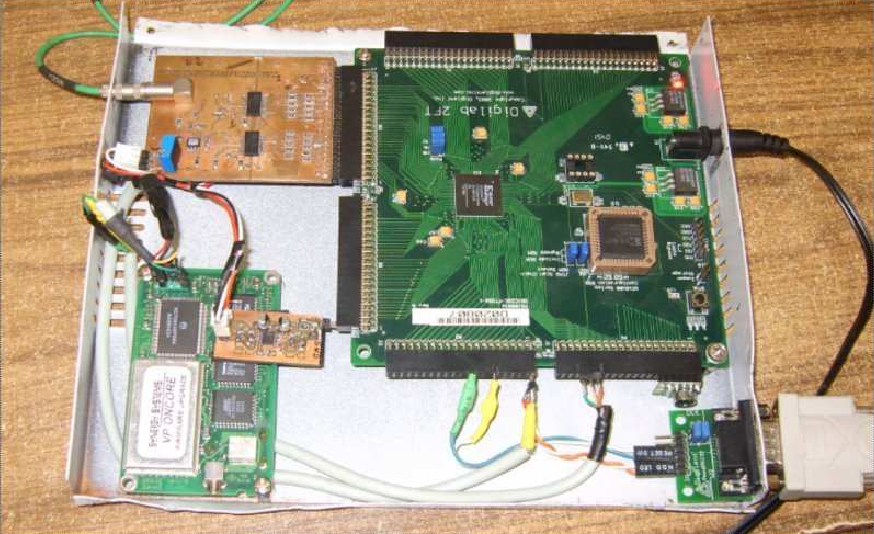
\includegraphics[scale=0.4]{images/mexico/sitelago-0A.png}
%\caption{New electronics for LAGO. The prototype can be operated at 100 or 200 MSPS.}
%\label{sitelago0A}
%\end{figure} 

The custom-made instrumentation for the DAQ system uses low power consumption,
it includes: A 4-channel ADC daughter-board with two dual 10-bit ADC chip
from Analog Devices, this chip was the AD9216 that is a dual, 3 V, 10-bit,
105 MSPS analog-to-digital converter. The daughter-board is connected to a
second board with an FPGA, for real-time data processing (Nexys2 from Digilent
Inc.); This board is a powerful digital system design platform built around a
Xilinx Spartan 3E FPGA, with 16 Mb of fast SDRAM and 16 Mb of Flash ROM. The
Nexys2 board is ideally suited to embedded processors like Xilinx's 32-bit
RISC Microblaze. Communication and control are based on a small minicomputer
Raspberry PI model B 512MB with an ARM1176JZF-S 700 MHz processor, this mini-
computer is the main control between the host y the DAQ, and it is used for
interconnection with the surface detector modules, the mother board has two
ways of communication with the host, the first one uses a serial port with a
typical communication rate around 115200 bits per second and the second one
uses a USB port with a higher communication speed.

A pressure and temperature sensor, (HP03D from Shenzhen Hope Microelectronics
Co. Ltd.) which includes a piezo-resistive pressure sensor and an ADC interface,
providing 16 bit word data for pressure and temperature related voltage, is
connected to the FPGA board. The algorithms developed use advanced digital
signal processing techniques and particularly digital pulse processing, where
the purpose of the pulse processing is to perform on-line signal processing
on the digitized signals directly to minimize the data transfer size, these
algorithms are implemented on the FPGA using Hardware Description Language
(VHDL) and C Language for the Microblaze processor, these algorithms can be
reprogrammed at any time. Each event is tagged with precise GPS time tags using
an embedded GPS receiver with 1 PPS (one pulse per second) synchronized with
UTC within an uncertainty of 50 ns (Motorola Oncore UT+ GPS receiver), see
figure \ref{fig:electronics-m}. The bitstream firmware of the DAQ system
resides permanently on the Flash ROM chip located on the mother board and it
gets downloaded into the FPGA upon power on.

%On the PC side we use Perl and Python under Linux to process,
%store and display the data acquired. Finally, we use ROOT programs to histogram
%and analyze the data.

\begin{figure}[t]
\centering
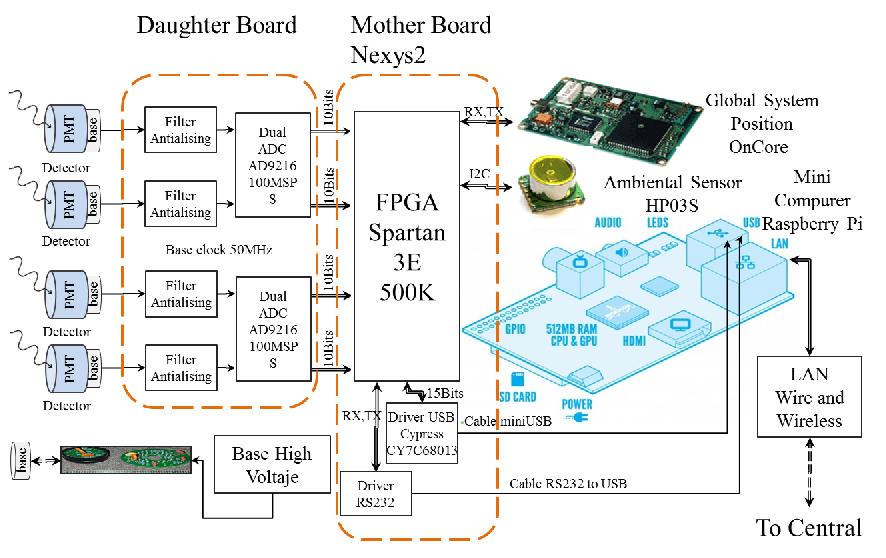
\includegraphics[scale=0.5]{images/mexico/sitelago-02.png}
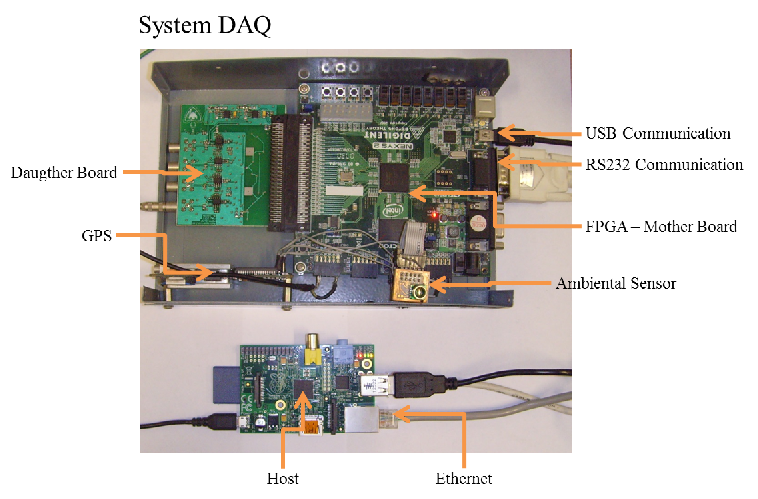
\includegraphics[scale=0.69]{images/mexico/sitelago-03.png}
\caption{Top: DAQ full blocks diagram, you can see the main parts of the DAQ.1.- Daughter Board 2.- Mother Board, and 3.- Host. Bottom: custom electronics designed for the LAGO mexican part of the collaboration, it can be operated at 100 or 200 MSPS}
\label{fig:electronics-m}
\end{figure} 


\section{The LAGO sites}\label{sec:sites}

As it was mentioned in previous sections, LAGO spans over many different
countries in Latin America. In this section we describe the sites according to
the location in each of the countries that have a LAGO detector. In
Fig.\ref{fig:lago-map}, a map of the Latin American region can be seen with the
sites marked where a LAGO WCD is in operation, to be installed in the 2014-2015
period or the sites in evaluation. Also the different countries are marke with
different colours.

\begin{figure}
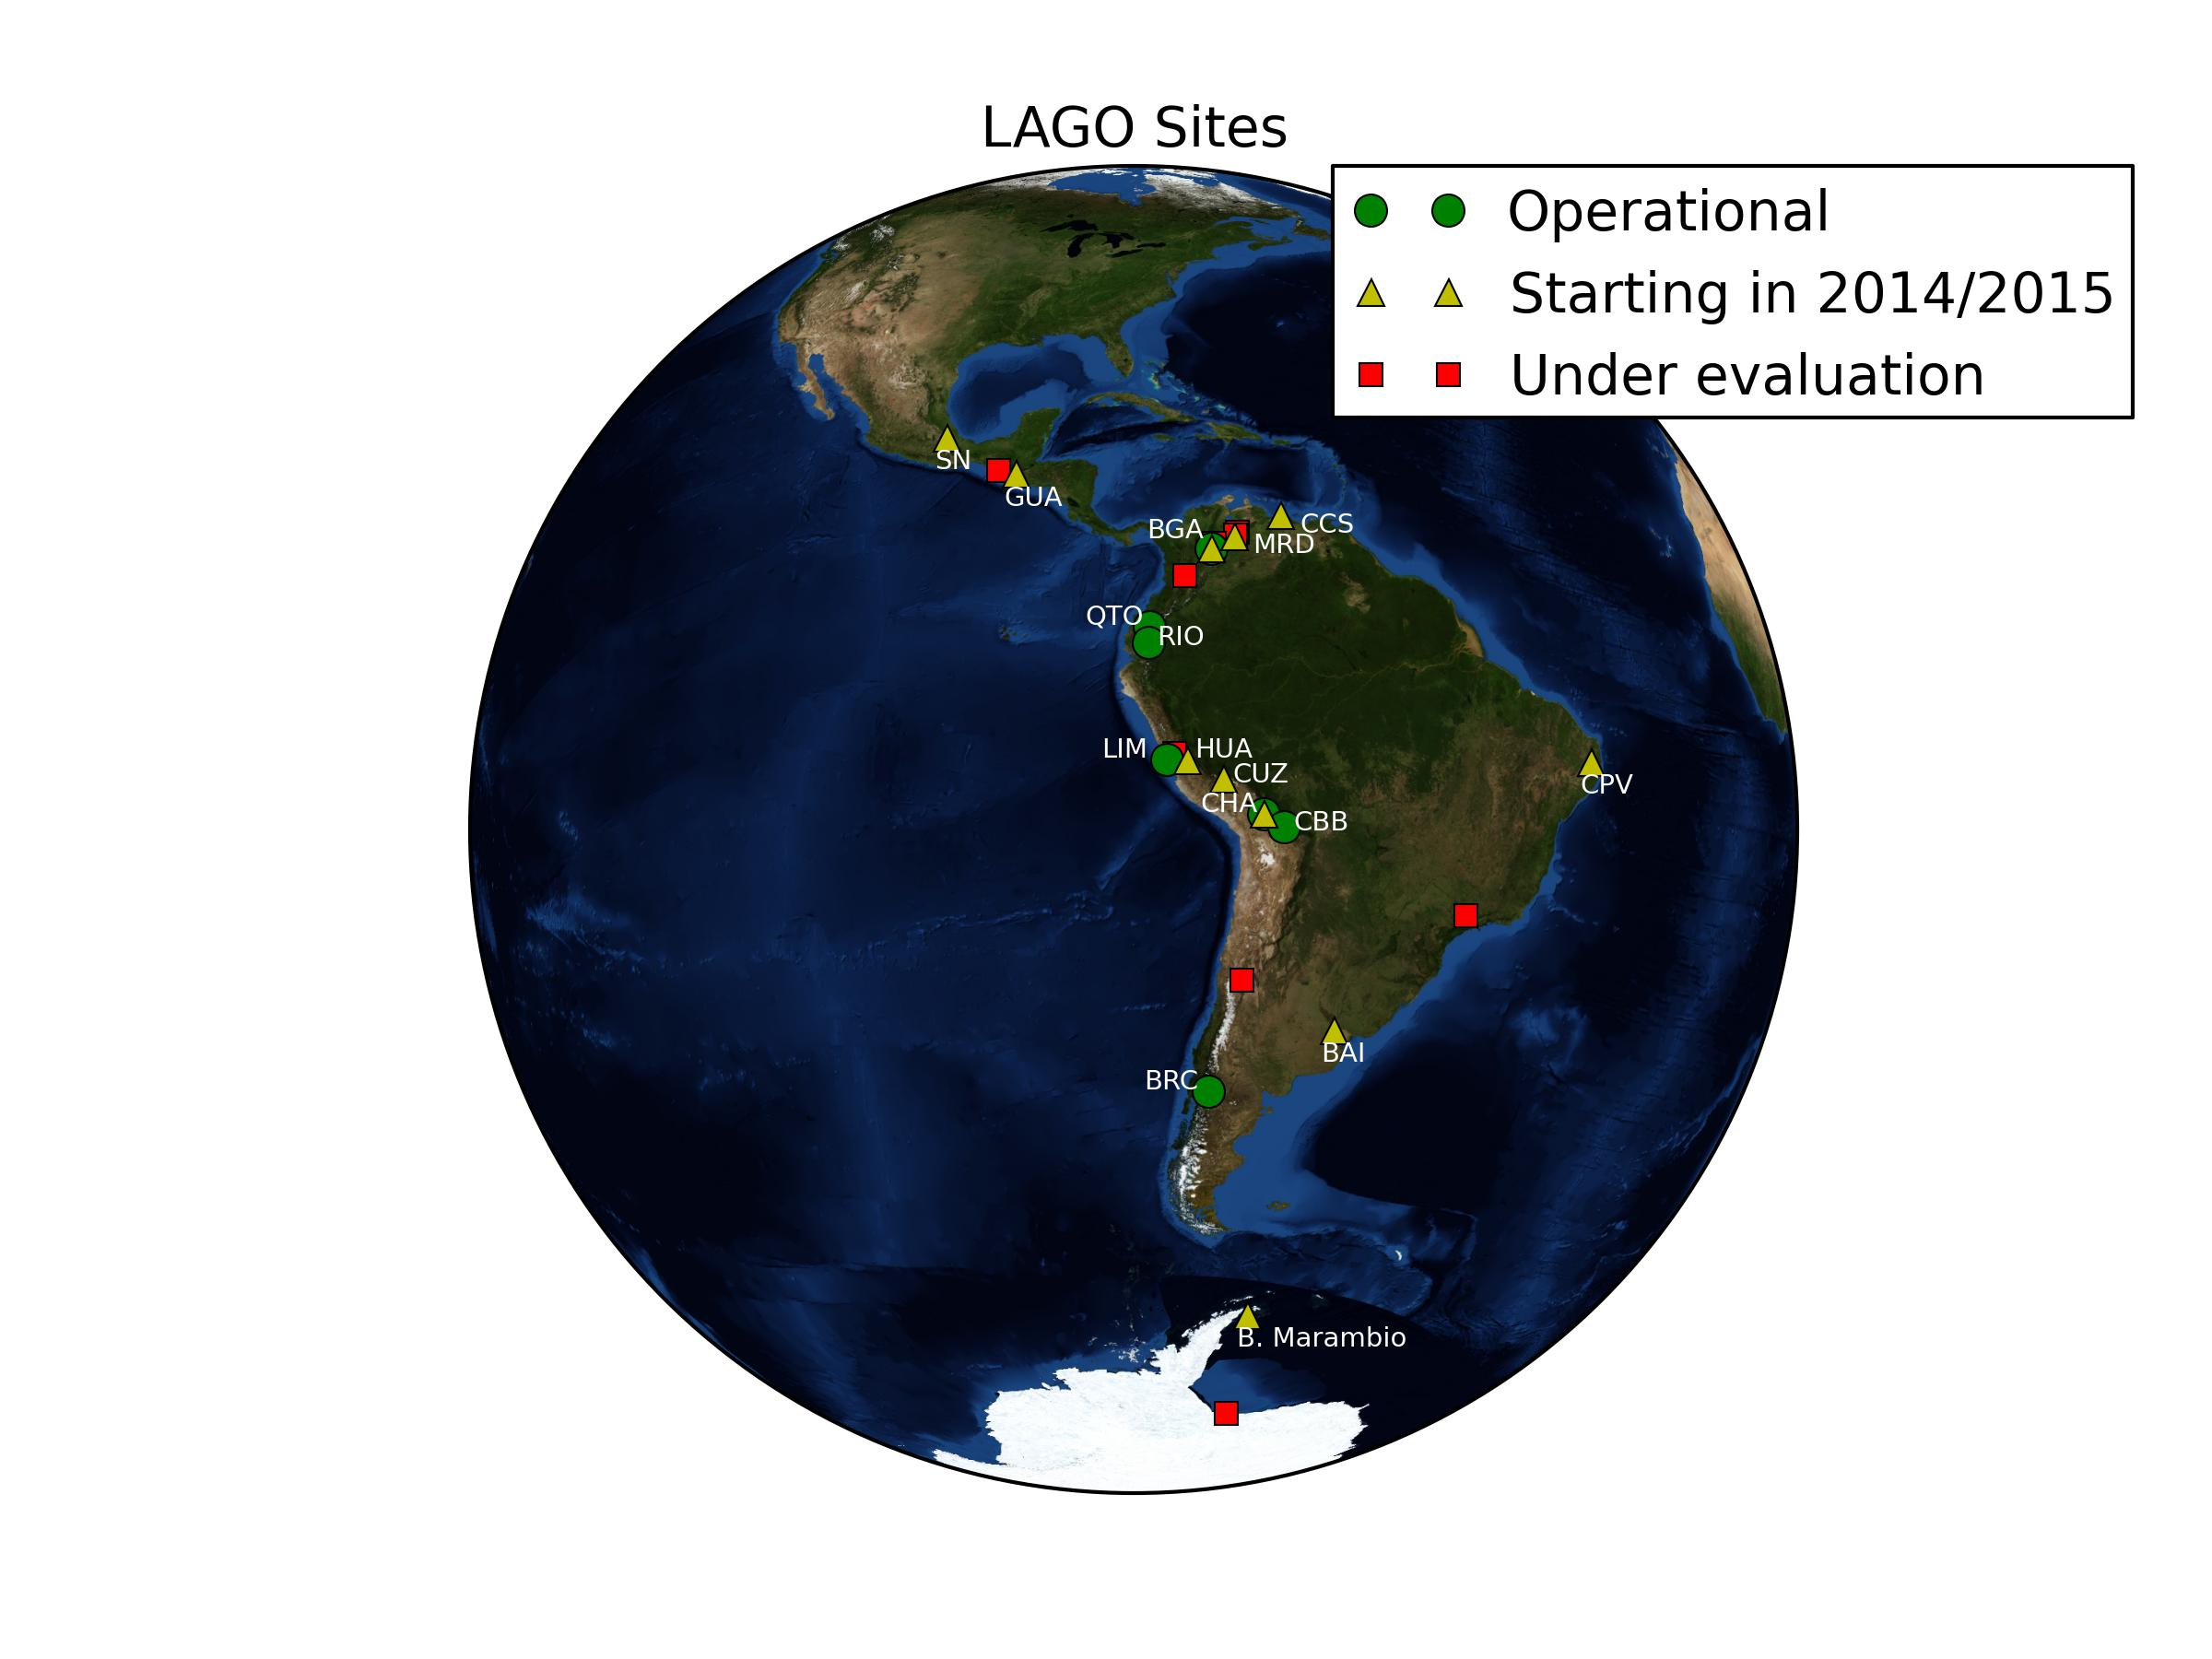
\includegraphics[width=.9\textwidth]{images/LagoMapa.jpg}
\caption{Google earth map showing all LAGO sites. For the color code label each
country that are in the LAGO collaboration. The markers shows if the detector
is operation at this day, is going to start measurements in the period
2014-2015 or the site is under evaluation to hold a WCD that will belong to the
LAGO network.} \label{fig:lago-map}
\end{figure}

To see the different sites, a compilation of the locations, detector size,
altitudes, rigidity cut off, latitude, longitude, and general observations are
made in table \ref{tab:locations}.

venezuela

\begin{table*}[!ht]
\begin{center}
\setlength{\tabcolsep}{0.2em}
\begin{tabular}{|c|c|c|c|c|c|c|c|c|}
\hline
\multirow{2}{*}{Country} & \multirow{2}{*}{Site} & Number of & Altitude & Altitude & Rigidity & Latitude &Longitude& \multirow{2}{*}{Observations}\\
 & & WCD & [m a.s.l.] & [g/cm$^2$] & cut off [GV] & [deg] & [deg] & \\
\hline
\hline
 \multirow{3}{*}{Argentina} &Bariloche &3&850 & & & 41.15 S& 71.30 W & \\
&Buenos Aires &1& 10& & 8.4$\pm$0.6 & 34.54 S & 58.44 W & \\
&Marambio &1& 200 & & & 64.24 S & 56.62 W & \\
\hline
Bolivia & Chacaltaya & 3 & 5240 & 530 & 12.5 & 16.35 S& 68.13 W & \\
\hline
Colombia & Bucaramanga & 1 & 956 &  & & 7.14 S& 73.12 W & \\
\hline
Ecuador & Chimborazo & 1 &  &  & & 1.81 S& 78.74 W & \\
\hline
Guatemala & Guatemala & 1 & 1490 &  & 8& 14.63 S& 90.59 W & \\
\hline
México & Sierra Negra & 4 & 4550 &  & 9& 18.16 S& 97.95 W & \\
\hline
\multirow{3}{*}{Perú} & Lima & 2  &150  &  & & 12.10 S& 77.02 W& \\
 & Cusco & 1& 3400 &  & & 13.52 S& 71.96 W& \\
 & Huancayo & 1& 3370 &  & & 12.04 S& 75.30 W& \\
\hline
 \multirow{3}{*}{Venezuela} &Caracas-UCV &1& 900& & 11.29 & 10.49 S & 66.89 W & \\
&Caracas-USB  &1& 1200& & 11.30 & 10.41 S & 66.88 W & \\
&M\'erida-ULA &1& 1893& &11.51 & 8.63 S & 71.15 W & \\
\hline
\end{tabular}
\caption{Table of the different locations of the LAGO sites.}
\label{tab:locations}
\end{center}
\end{table*}


\subsection{Argentina}\label{subsec:arg}
%\subsubsection{Bariloche}

The site in Bariloche is located at the Centro Atómico Bariloche, see table
\ref{tab:locations}. As mentioned in section \ref{sec:electronics} the
Bariloche group has developed the electronics for the LAGO project in
collaboration with the Mexico group. The detectors in this site are mostly used
to test and improve the data acquisition software and hardware since 2006. 
In addition, the use of these WCD were of outmost importance for the first
space wheather studies within the LAGO collaboration (see section
\ref{sec:science}).

%\subsubsection*{Detectors description}
Three different WCD have been assembled. Nahuelito was the first detector build in 2006
and together with Boyita are made of commercial plastic water tanks. Recently a
stainless steel commercial water tank has been used in the construction of
Sputnik. The latter will serve as a prototype for the Antarctic site detector
(section \ref{sec:antartica}). Geometry and dimensions details of these three
detectors are shown on figure \ref{fig:bar-tanques}.

\begin{figure}[h!]
\begin{center}
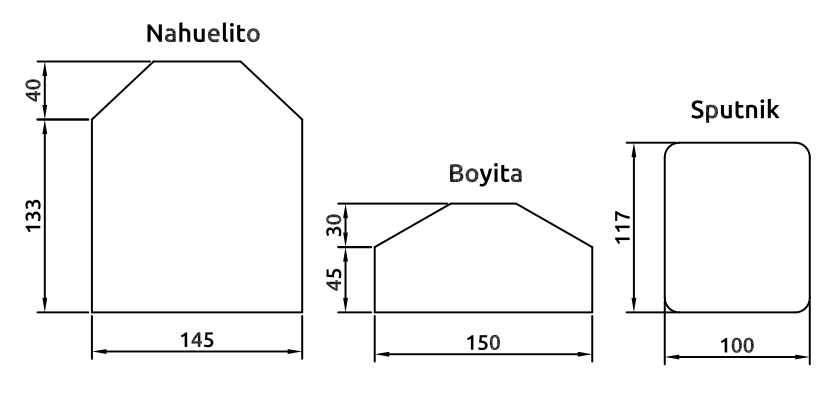
\includegraphics[width=0.8\textwidth]{images/argentina/tanques-bariloche.png}
\caption{Geometry and dimensions of the Bariloche site detectors (all units in cm).} 
\label{fig:bar-tanques}
\end{center}
\end{figure}

All detectors have an inner liner made of Tyvek$^{\textregistered}$ and one PMT mounted on top.
Both Nahuelito and Boyita have 8\,'' Hamamatsu R5912 PMTs while Sputnik has an
8\,'' Electron Tube Limited 9353KB PMT. Because of the good water quality of Bariloche
no purification process was implemented and tap water is used directly. The possibility of
doping the water with Amino-G (NH$_2$C$_{10}$H$_5$(SO$_3$H)SO$_3$Na) as wavelength shifter
to improve the signals has been explored in all the Bariloche detectors. 
 
%\subsubsection*{Detectors performance}

During the last years the use of the detectors has been shared with
experimental physics courses for Balseiro Institute undergraduate students.
Currently only Nahuelito is used exclusively for the LAGO project. In this
section different results are presented using the three detectors to showcase
their performance.

Muon decay can be observed using WCD by looking at the histogram of time
difference between consecutive events as shown on figure \ref{fig:bar-data},
left.  Two different regions can be seen. At large time differences the
exponential distribution corresponding to the arrival of uncorrelated particles
from the background of secondary cosmic rays. At small time differences another
exponential distribution with a characteristic time $\approx$2\,$\mu$s
corresponding to muon decay \cite{}.

Charge and amplitude histograms are used to calibrate the detectors. The
maximum of the muon hump, corresponding roughly to verticals muons, can be used
to define the VEM (Vertical Equivalent Muon). $1\,$VEM is the average signal of
a vertical and central muon. The final energy calibration of the detectors can
be done knowing the average energy deposited by a vertical muon. A typical
charge histogram of Boyita can be seen in figure \ref{fig:bar-data}, center.

During the construction of Sputnik the improvements on the signals due to the
inner Tyvek$^{\textregistered}$ liner and the addition of Amino-G to the water
was checked. Comparison of average signals taken with the stainless steel tank
only and the addition of the inner liner and Amino-G (6\,mg/l) can be seen in
figure \ref{fig:bar-data}, right. All the signals were taken using an oscilloscope
with a trigger rate of approximately 100\,Hz. Using the LAGO data acquisition
electronics with a sampling rate of 40\,MHz the charge-amplitude ratio goes
from 1 in the case of bare stainless steel to approximately 1.5 with the
addition of the Tyvek$^{\textregistered}$ liner and to approximately 2 doping
the water with Amino-G.  

\begin{figure}[h]
 \begin{center}
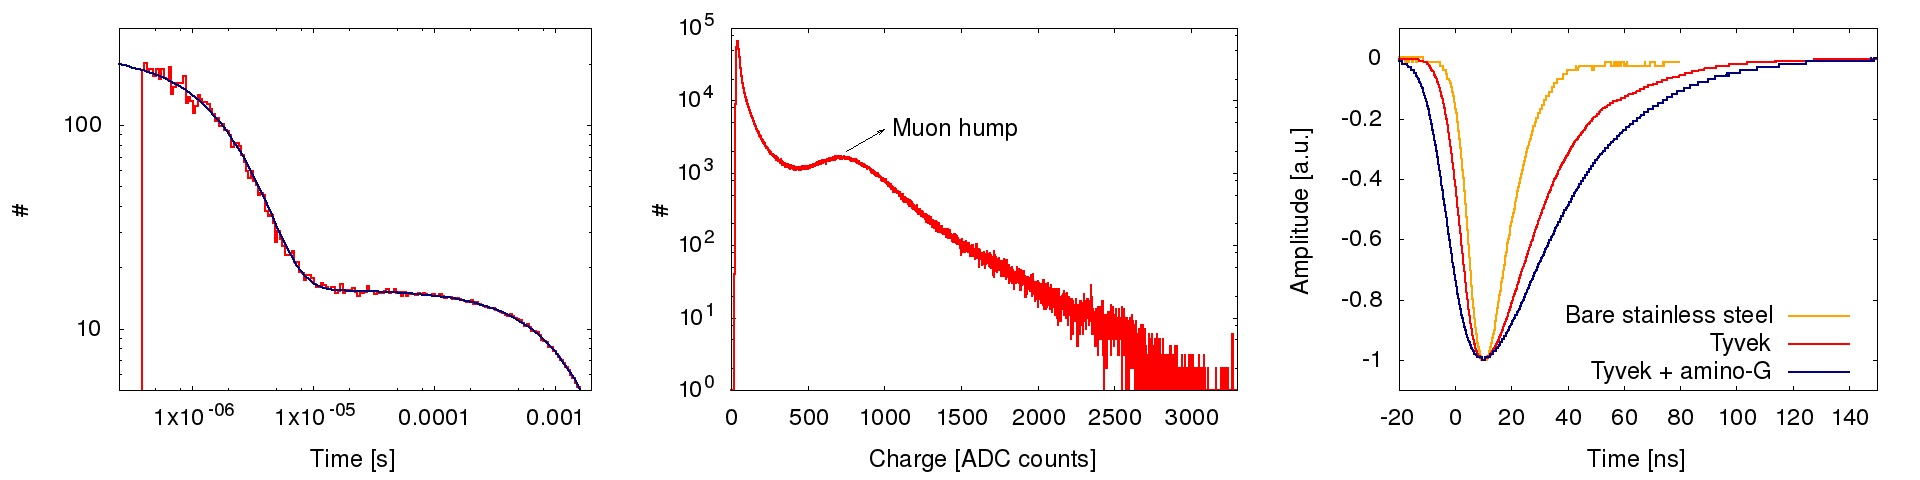
\includegraphics[width=\textwidth]{images/argentina/data.png} \caption{Left: histogram
of time difference between consecutive events using Nahuelito. A fit of the sum
of two exponential functions corresponding to muon decay and the arrival of
uncorrelated particles of the background can be observed. Center: one hour
typical charge histogram using Boyita. Right: Comparison of average traces with
the stainless steel tank only and after the addition of the
Tyvek$^{\textregistered}$ liner and Amino-G. A significant improvement of the signal
is observed.} \label{fig:bar-data} 
\end{center}
\end{figure}

The addition of Amino-G as wavelength shifter significantly improves the
signals of WCD. However a systematic study of the aging of Amino-G doped water would be
necessary before deciding on its use in all LAGO detectors.

%\subsubsection{Buenos Aires}

The detector located in Buenos Aires is at the campus of the Universidad de
Buenos Aires (UBA), in the building of the Instituto de Astronomía y Física del
Espacio (IAFE), se table \ref{tab:locations}. It is used mainly to test the
remote operation and low level of local maintenance requirements, for those
detectors requiring high levels of autonomy. This detector is used also to test
resistance to extreme conditions (e.g., extreme low temperatures).  The group
of Buenos Aires is the responsible of the project 'LAGO in Antartic' (see
Section \ref{sec:antartica}).

%\subsubsection*{Detector description}

\begin{figure}[h!]
\begin{center}
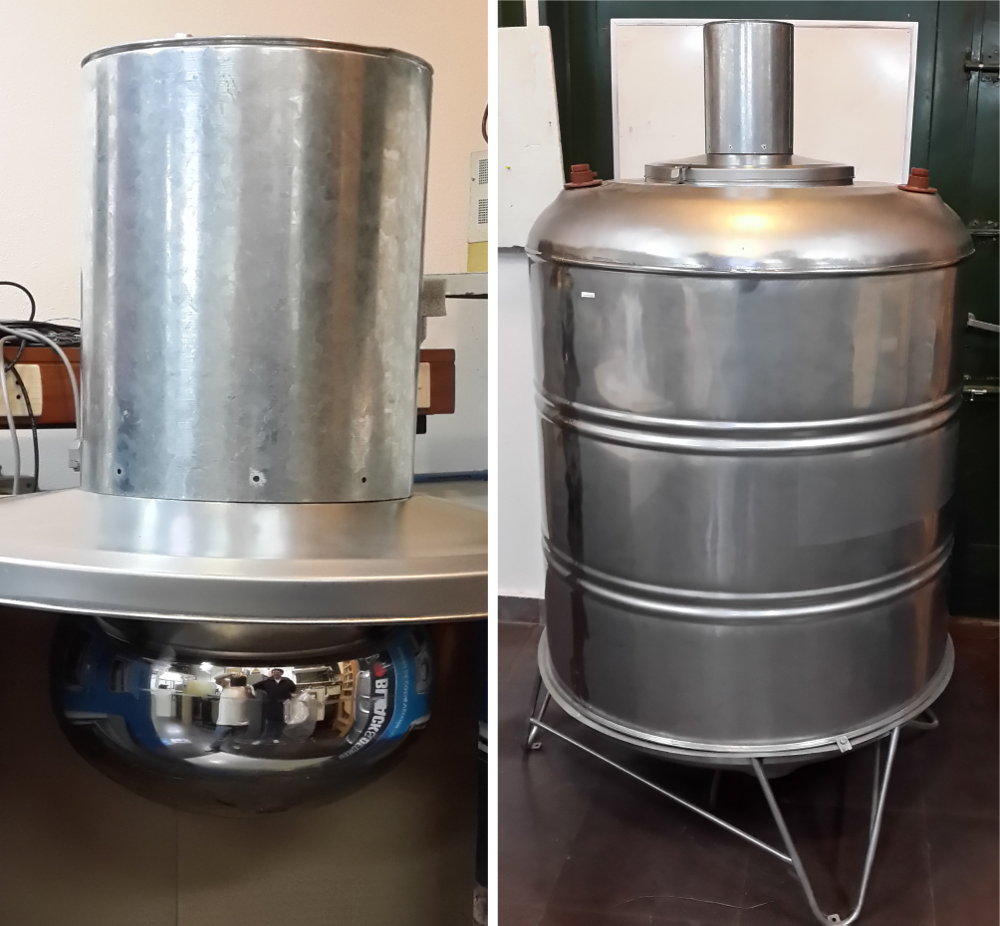
\includegraphics[width=0.8\textwidth]{images/argentina/neurus.png}
\caption{Neurus detector. Left: support for the PMT and its electronic base
(connectors are above [not shown]). Right: The detector with the base of the
PMT (isolated for humidity) above and outside the water container, inside the
tall top hat.}
\label{fig:neurus}
 \end{center}
\end{figure}

A WCD, labeled 'Neurus', was constructed and it is a prototype for the detector
to be installed at the first site of LAGO-Antartica.  The water container is a
stainless steel commercial water tank.  The geometry and dimensions of the
water container are the same as Sputnik detector at Bariloche (see right side
of Figure \ref{fig:bar-tanques}).  It has an inner liner made of
Tyvek$^{\textregistered}$ and one PMT of 9'' PHOTONIS XP1805 mounted on its top.
The water is purified using a standard commercial filter for human consuming,
removing the chlorine present in the water of the net.  In order to minimize
the presence of humidity in the electronic, the base of the PMT is isolated in
a tall top hat, outside the water recipient (see Figure \ref{fig:neurus}). At
the moment, Neurus is used exclusively for the LAGO project, and we plan to
share it in the near future for experimental undergraduate physics courses for
students from the physics department of the Universidad de Buenos Aires.

%\subsubsection{LAGO in Antartica}
\label{sec:antartica}

For developing scientific research associated with the branches of Space
Physics and Space Weather in LAGO (see section \ref{sec:science}), low values
for rigidities cut-off are desirable.  Sites located at low magnetic latitudes
are then favorable for installing new LAGO detectors. Antartica is then an
excellent place to this purpose.  In this section, we describe the project
'LAGO in Antartica', a project to install detectors inside the Argentina sector
of Antartica.

%\begin{figure}[h!]
%\begin{center}
%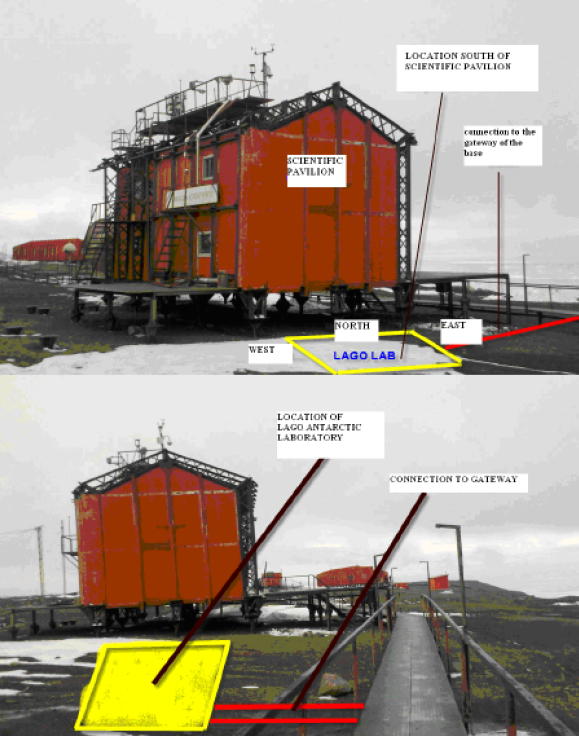
\includegraphics[width=0.8\textwidth]{images/argentina/site_labo_marambio.png}
%\caption{Location of the proposed LAGO node at
%Marambio Station .}
%\label{fig:marambio-location}
%\end{center}
%\end{figure}

The activities developed for selecting and planning the antartic site, as well
as for constructing the laboratory are included into a frame of collaboration
between the Instituto Ant\'artico Argentino (Direcci\'on Nacional del
Antartico, IAA/DNA), the Instituto de Astronomia y Fisica del Espacio (IAFE,
UBA-CONICET), and the LAGO network collaboration.

After our campaign during the austral summer of 2011 to determine the best site
location for the LAGO laboratory in Antartica, we concluded that due to the
possibilities of constructing a new building and due to the infrastructure
available, the Marambio base is the best option for locating the first
Antarctic LAGO node.

For safeguard and operational resources reasons, it was decided to mount the
module near the scientific pavilion. The new LAGO laboratory will be located
in such way that will be possible to access through by a gateway from/to the
already installed scientific pavilion. This is important because our study of
winds (intensities and directions) predict the existence of strong winds during
winter time and the idea is that the hard outside enviroment do not affect the
maintenance of the detectors. The following photos show the place on figure
\ref{fig:marambio-location}.

Due to the low temperatures at Marambio, the cherenkov detectors should be
protected at an over zero Celsius environment.  A laboratory to locate the
detectors is projected to be constructed. 
% The plan floor of the laboratory to
%be constructed is shown in Figure \ref{fig:planfloor}.

%\begin{figure}[h!] \begin{center}
%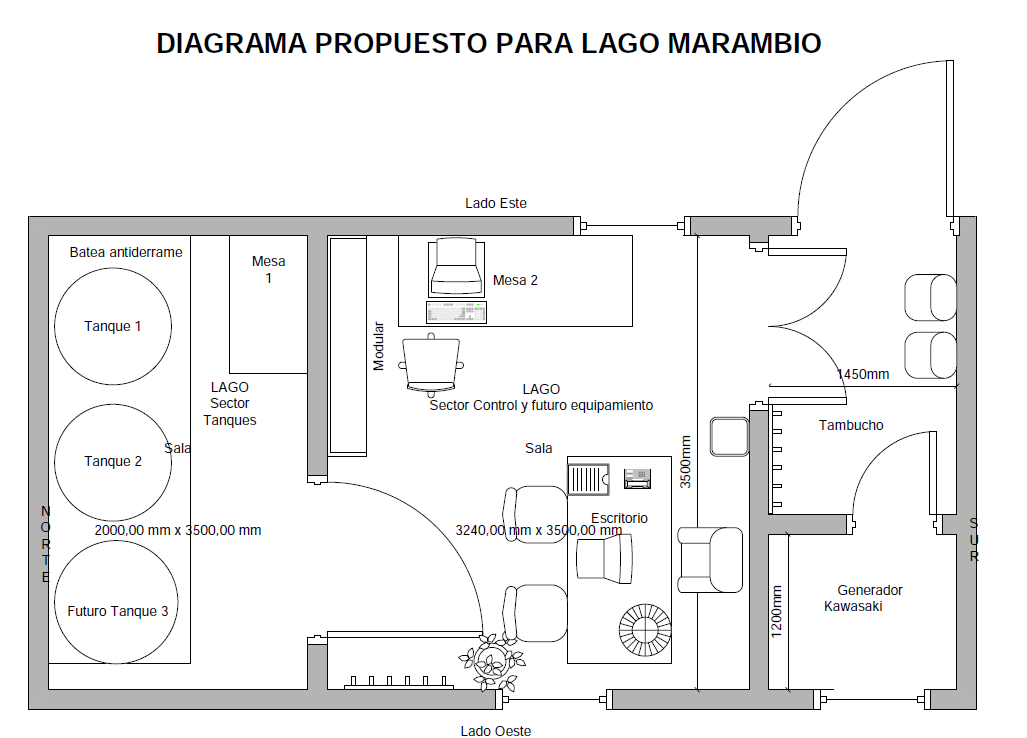
\includegraphics[width=0.8\textwidth]{images/argentina/plano_labo_marambio.png}
%\caption{Plan floor of the LAGO laboratory at Marambio .} \label{fig:planfloor}
%\end{center} \end{figure}

The election of this site is also supported from a series of numerical
simulations of different conditions for the arrival of cosmics rays at this
site.  The cutoff rigidity at Marambio, for quiet geomagnetic
conditions, is R$_c^{Mr}$ = (2.3 $\pm$ 0.2) GV \cite{Masias2014}.
It has a dependence with the geomagnetic activity and Marambio is magnetically
connected to the polar oval, consequently this site will be the first LAGO site
available to observe precipitation of particles from this region of the
magnetosphere.
Also, the study of the sensitivity of $R_c$ to geomagnetic storms at Marambio using
the Dst index as a proxy to quantify the strenght of the storm, finding a
relative rate of change of $\frac{1}{Rc}\frac{\Delta Rc}{\Delta
Dst}=3\times10^{-3}$nT$^{-1}$ \cite{Masias2014}. 
%$1/Rc (\Delta Rc / \Delta Dst)$ at BsAs is $-0.1/nT$, and at Marambio is
%$-0.3/nT$.
%This result can be seen in Figure \ref{fig:bsas_marambio}, where values for
%Buenos Aires are also included for comparison; 
%Changes in R$_c$ imply that lower rigidity particles can reach Earth during periods active of geomagnetic storms.

%%\begin{figure}[h!]
%%\begin{center}
%%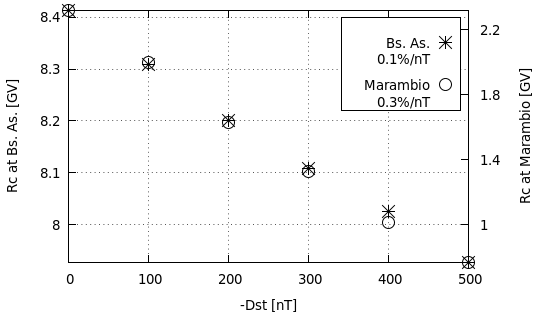
\includegraphics[width=0.8\textwidth]{images/argentina/dst_vs_Rc_bsas_and_marambio_LAGO.png}
%%\caption{Rigidity cut-off for different global geomagnetic activity (Dst index
%%used as proxy) for Buenos Aires and Marambio base in Antartica. Adapted from \cite{Masias2014}.}
%%\label{fig:bsas_marambio}
%%\end{center}
%%\end{figure}
%%
  %1
\include{sites/brazil-sites}     %2
\subsection{Bolivia}\label{subsec:bol}

Three WCD are operating, since 2009, at the cosmic ray laboratory on mount
Chacaltaya, near the city of La Paz, Bolivia. The high elevation of the
laboratory (see table \ref{tab:locations}) improves the sensitivity of a WCD to
low energy showers with respect to a WCD with similar characteristics operating
at sea level.

Each of the WCD operating on mount Chacaltaya has a volume of pure water
contained in a cylindrical tank made of either plastic or fiberglass. The
volume of water is observed from above by an 8"  Electron Tubes
photomultiplier that collects Cherenkov photons emitted by the medium when
charged particles hit the detector. Moreover, the water has been
mixed with Amino-G, a chemical compound that acts as a wave length shifter,
thus effectively increasing the number of photons collected by the
photomultiplier. The walls of each tank are internally covered with a
reflective liner to improve the collection efficiency of the detector. Two
different materials were used as reflective liners, and their reflection
coefficients have been measured employing a violet led. Table \ref{tab:chars}
contains some of the characteristics for each of the WCDs operating at the
laboratory including the reflection coefficient. The configuration of the WCD
at the laboratory is sketched in the left side of figure \ref{fig:bolivia-wcd},
while the right side shows a picture of one the assembled detectors.

\begin{figure}[h!]
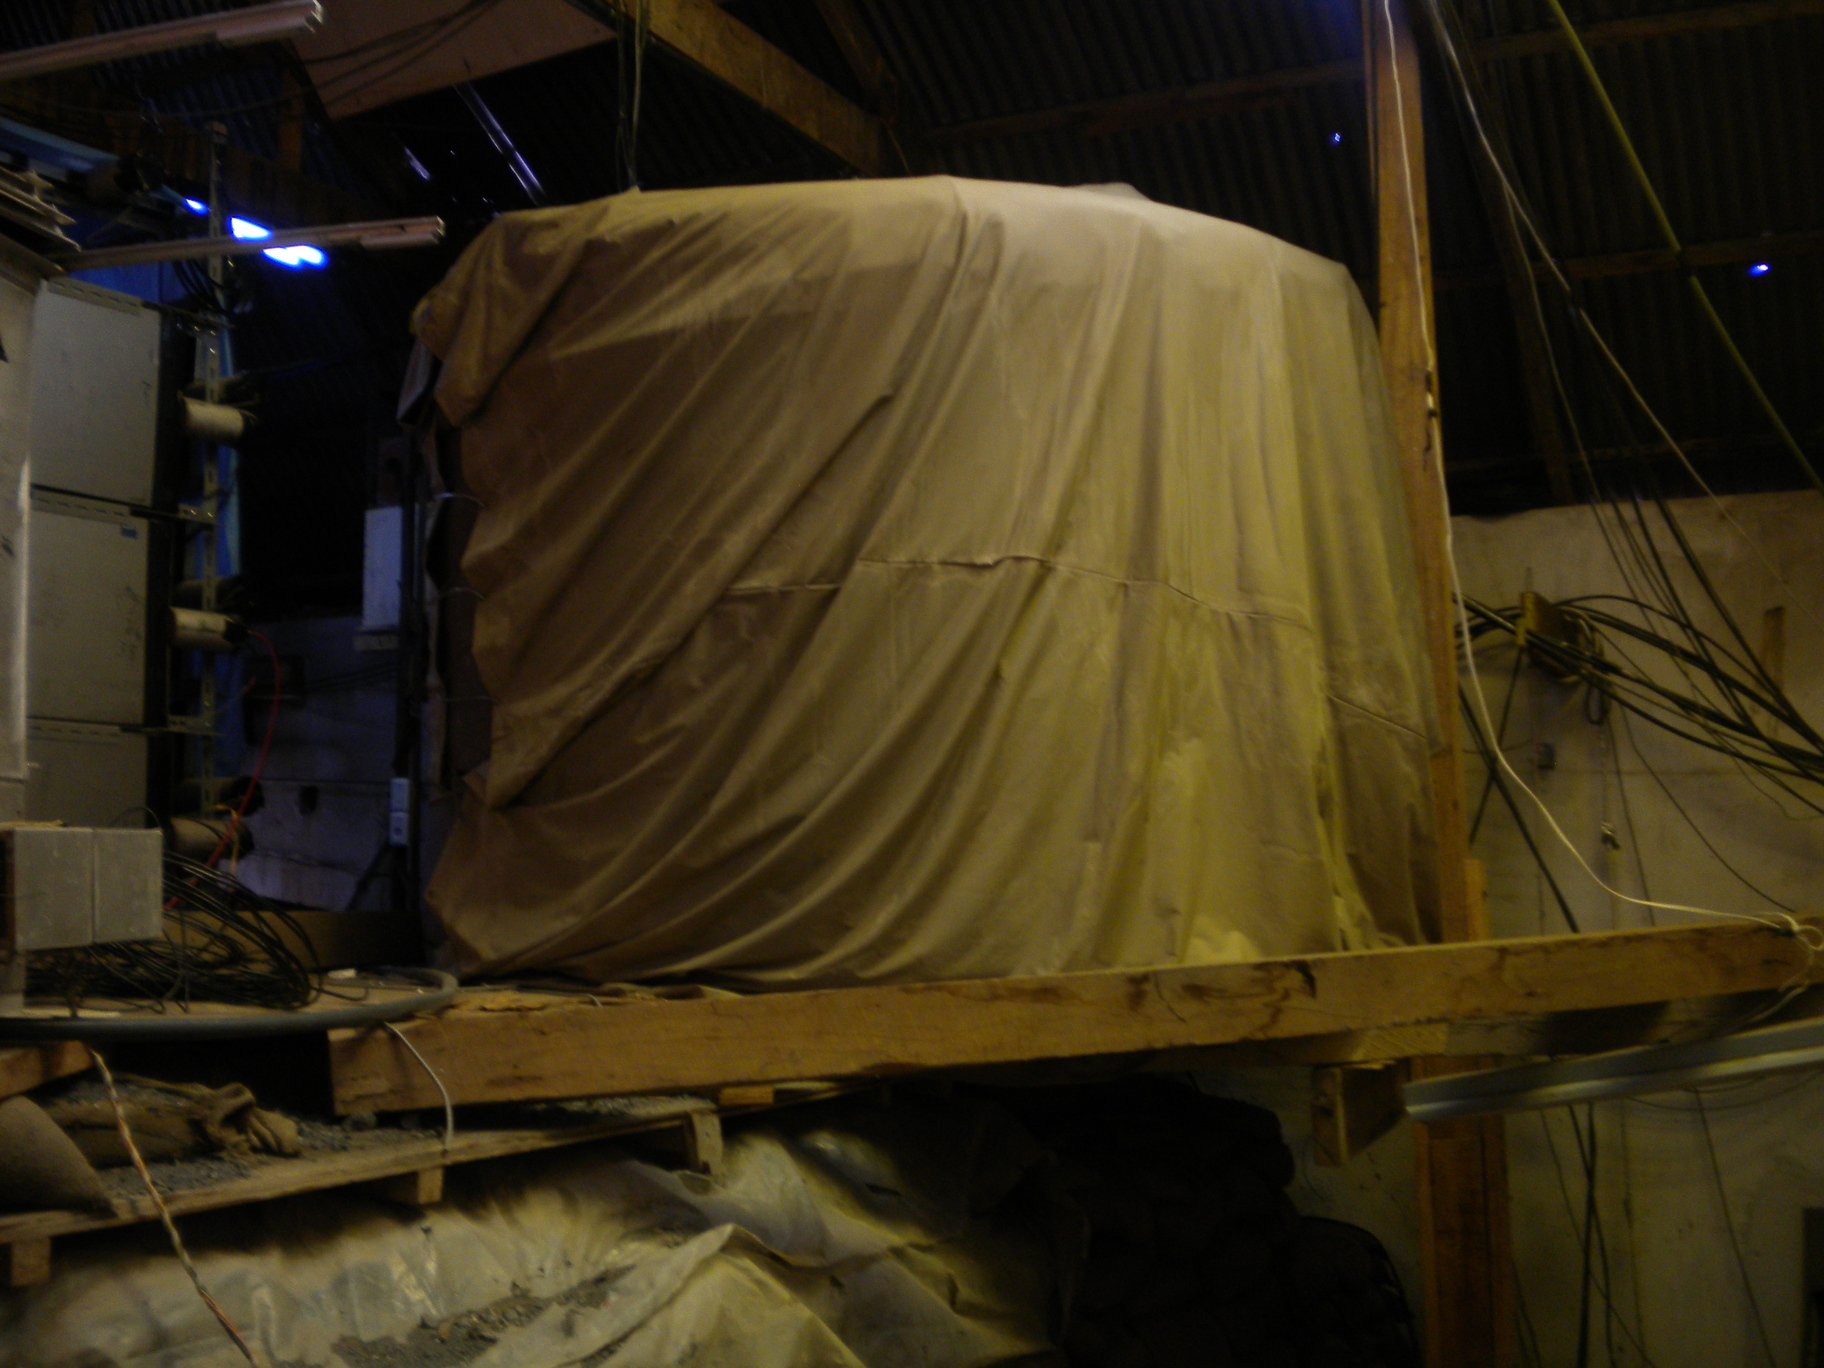
\includegraphics[width=0.5\textwidth]{images/bolivia/cha1139-m.jpg}
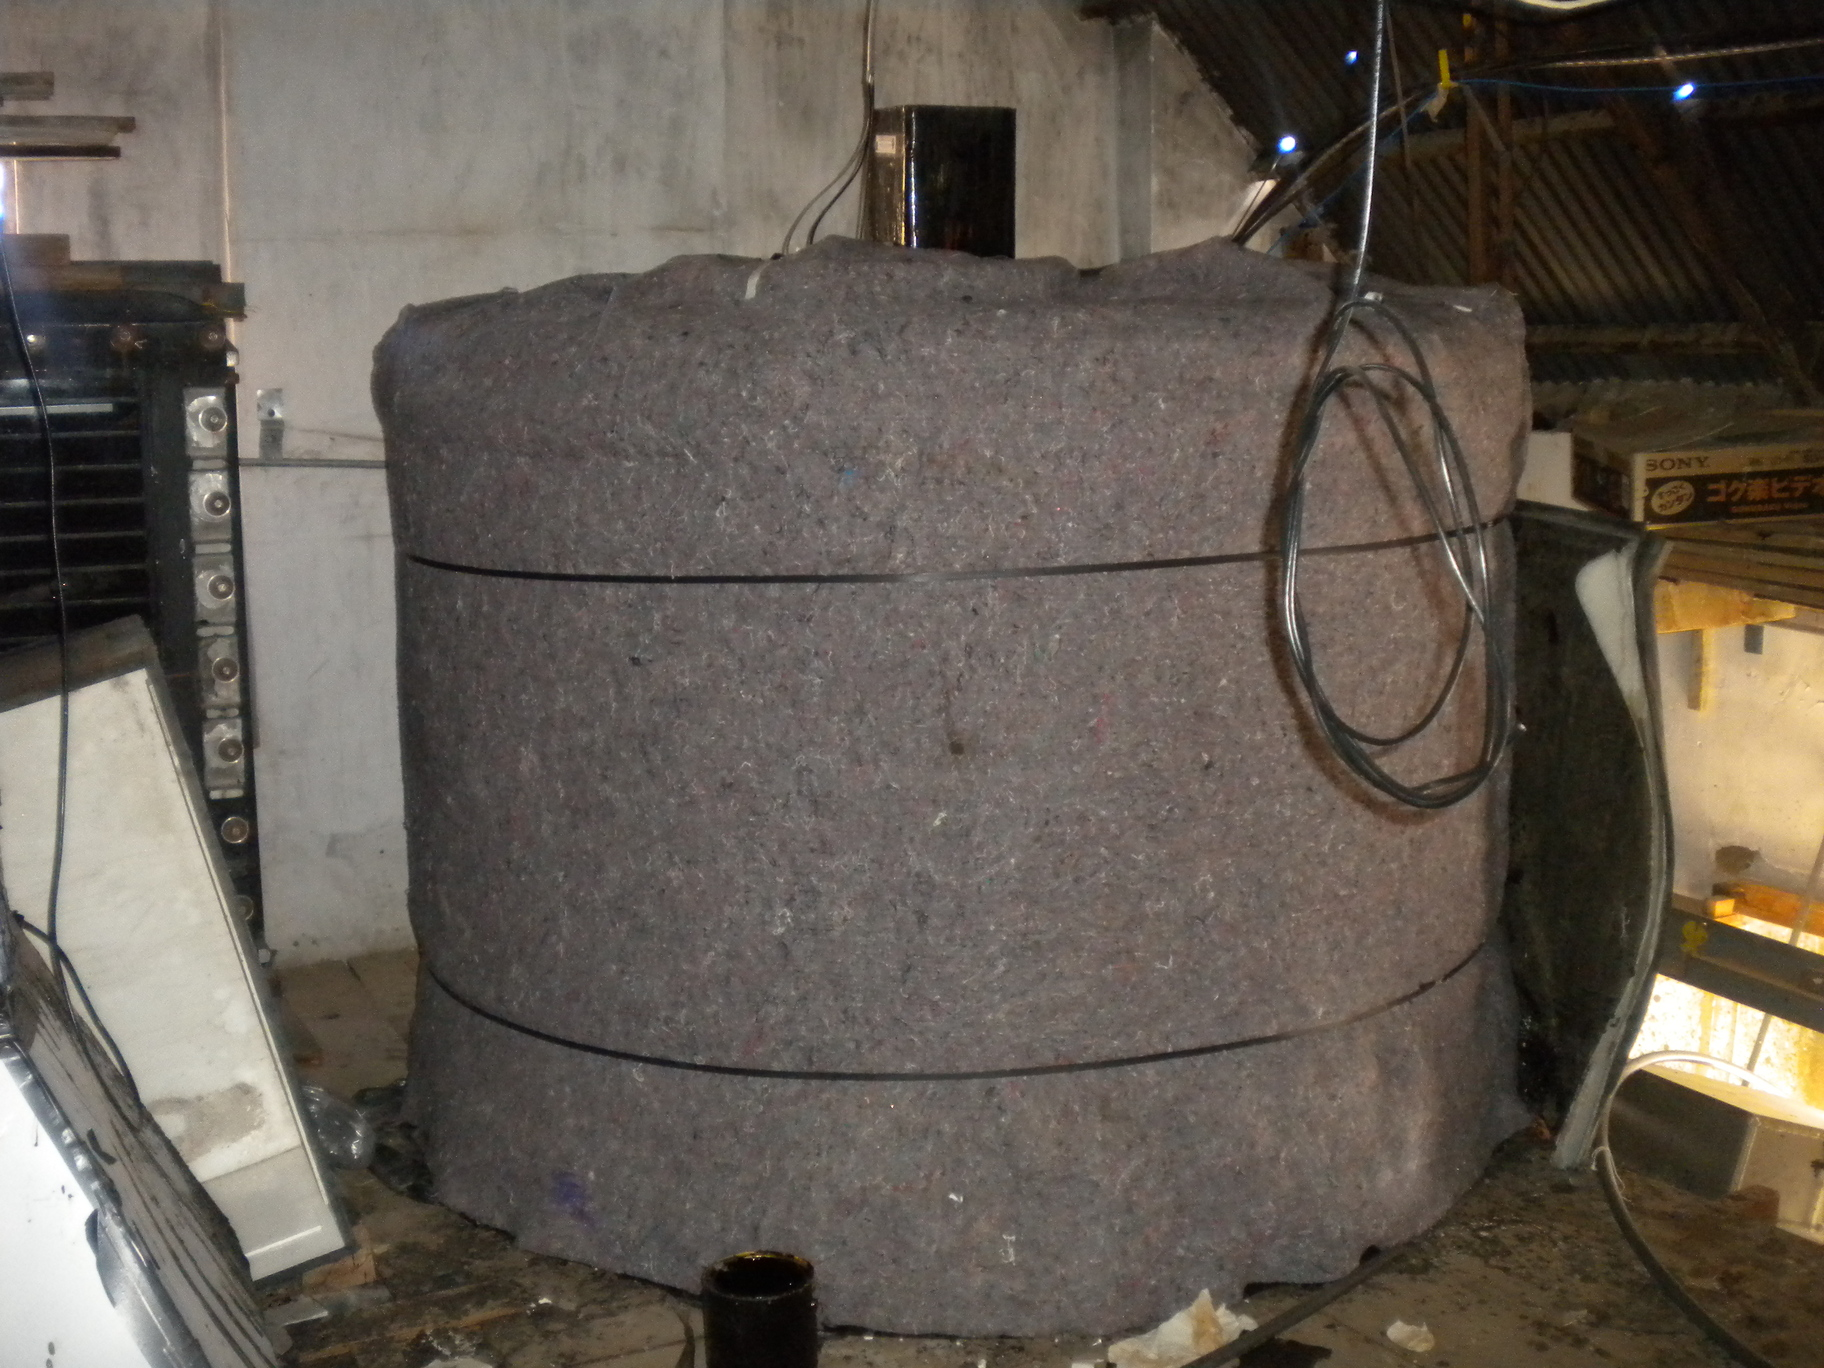
\includegraphics[width=0.5\textwidth]{images/bolivia/cha1140-m.jpg}
\caption{Pictures of two of the three WCD installed in mount Chacaltaya.}
\label{fig:bolivia-wcd}
\end{figure}

\begin{table}
\begin{center}
\begin{tabular}{|c|c|c|}
\hline
	& WCD1 & WCD2 \& WCD3\\
\hline
Diameter & $1.4\ \rm{m}$ & $2.2\ \rm{m}$\\
Water depth & $1.4\ \rm{m}$ & $1.5\ \rm{m}$\\
Water volume & $2200\ \rm{l}$ & $5300\ \rm{l}$\\
Amino G & yes & only in WCD2\\
Tank material & plastic & fiberglass\\
Liner material & Tyvek\textregistered & vinyl\\
Liner reflection coefficient & 0.8 & 0.9\\
Photomultiplier & 9353KB 8" & 9353KB 8"\\
\hline
\end{tabular}
\caption{Relevant characteristics of each WCD operating on mount Chacaltaya.}
\label{tab:chars}
\end{center}
\end{table}

Data acquisition is performed by means of a local station (LS), designed and
implemented at the Centro Atómico Bariloche, based on the data acquisition
electronics from the Pierre Auger Observatory. 
%The LS is basically built from a digitizer, a Nexys2 FPGA and a GPS clock
%although not functional at the time of writing. The digitizer has three input
%channels for analog signals ($50\ \rm{\Omega}$ impedance), an amplifier and a
%10 bit ADC with a sampling rate of $40\ \rm{MHz}$, that receives the signal
%coming from the photomultipliers. The sampling rate corresponds to a sampling
%period of $25\ \rm{ns}$. 
By means of the FPGA it is possible to connect the LS to pressure and
temperature sensors, but this feature is not implemented at the laboratory on
mount Chacaltaya at the time of writing. The FPGA operates at a rate of 40\,MHz
and it communicates with a standard PC running a Linux version. The
communication between the LS and the PC takes place via the USB port employing
the USB 2.0 protocol, achieving a transmission rate of 400\,MBps. The high
voltage required for the operation of the photomultipliers is controlled
employing a DAC and a pulse width modulation technique. A typical pulse
obtained from a WCD is shown in figure \ref{fig:bolivia-res1}, top panel.

\begin{figure}
\begin{center}
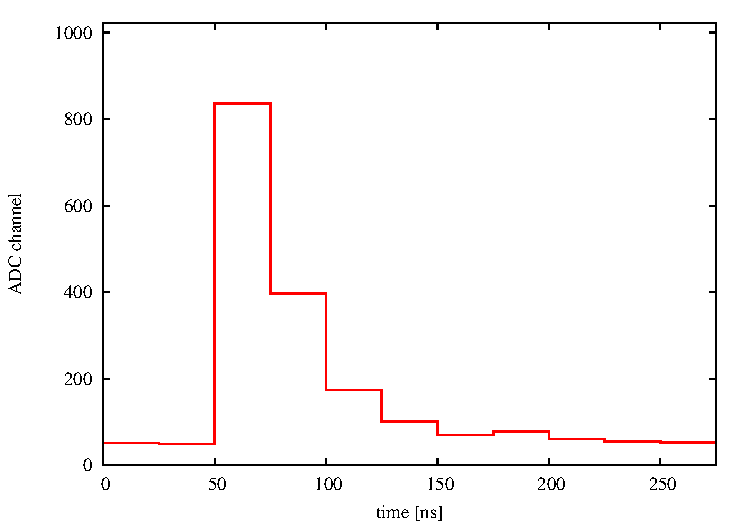
\includegraphics[width=0.6\textwidth]{images/bolivia/pulse.pdf}\\
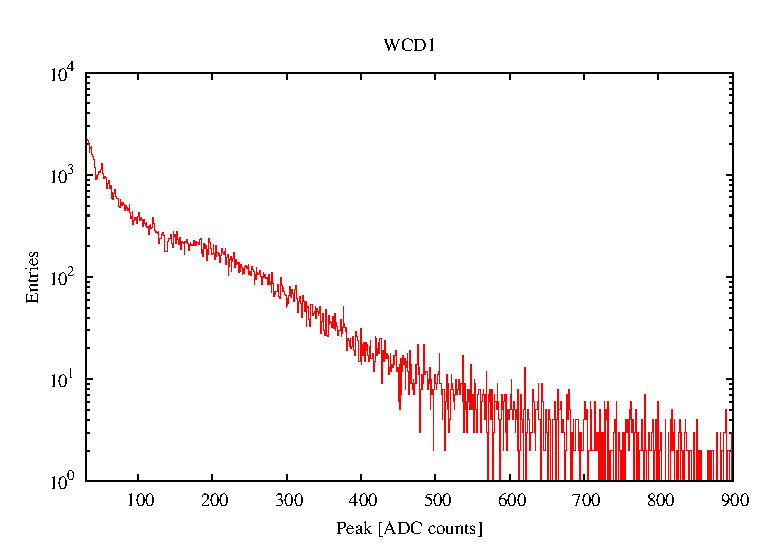
\includegraphics[width=0.49\textwidth]{images/bolivia/peakhist1.eps}
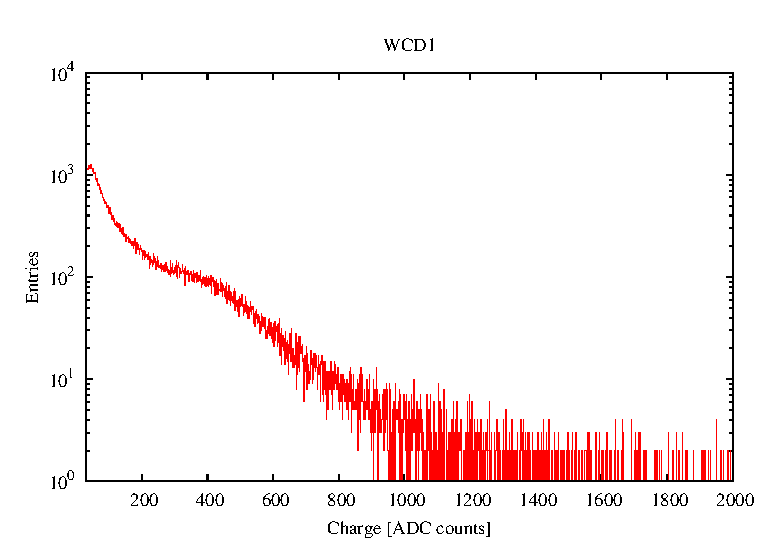
\includegraphics[width=0.49\textwidth]{images/bolivia/chargehist1.eps}
\end{center}
\caption{Top: A typical pulse shape obtained from a WCD. Bottom: Typical peak (left) and charge (right) histogram from one of the WCD located in mount Chacaltaya.}
\label{fig:bolivia-res}
\end{figure}

Two histograms are filled on a minute basis on each of the WCD. The first
histogram is filled with entries corresponding to the peaks (i.e. highest pulse
value) of the pulses received during a minute. The second histogram is filled
with entries corresponding to the charge (i.e. the integrated signal) of the
pulses. Two sample histograms are shown in figures \ref{fig:bolivia-res}, left
bottom and \ref{fig:bolivia-res}, right, corresponding to the WCD1. The muon
hump expected in the charge histogram is visible in the histogram, although not
as clearly as in a WCD located at sea level (see, for example, fig.
\ref{fig:bar-tanques} in section \ref{subsec:argen}. This is due to the
contribution of the electromagnetic component of showers (i. e. gamma rays and
electrons) which is dominant at very high altitudes.

As already noted, there are three WCD currently operational on the laboratory
at mount Chacaltaya and it is expected to have a new WCD operating at the
Higher University of San Simón in the near future, at the city of Cochabamba,
located on a valley with an elevation of almost 2600\,m.a.s.l.
    %3
\subsection{Colombia}\label{subsec:col}

\subsection*{Detector Description}

Colombia WCD, Guane-3, share similar characteristics with other LAGO WCDs.
Located at Bucaramanga in the Universidad Industrial of Santander, it is a
cylindrical reservoir filled with high quality purified water up to a level of
55 cm, and 103 cm of radio, and with a area of detection of 2.61m$^2$. The
water is contained in a reflective and diffusive bag, made of
Tyvek$^{\textregistered}$. The water volume is overlooked by a single Hamamatsu
photomultiplier tube of 8'' with a 25\% efficiency at 400\,nm. A picture of the
detector is showed in Fig. \ref{fig:Guane3WCD}. The electronics is the same
developed by the Bariloche group. 

\begin{figure}[h!]
\begin{center}
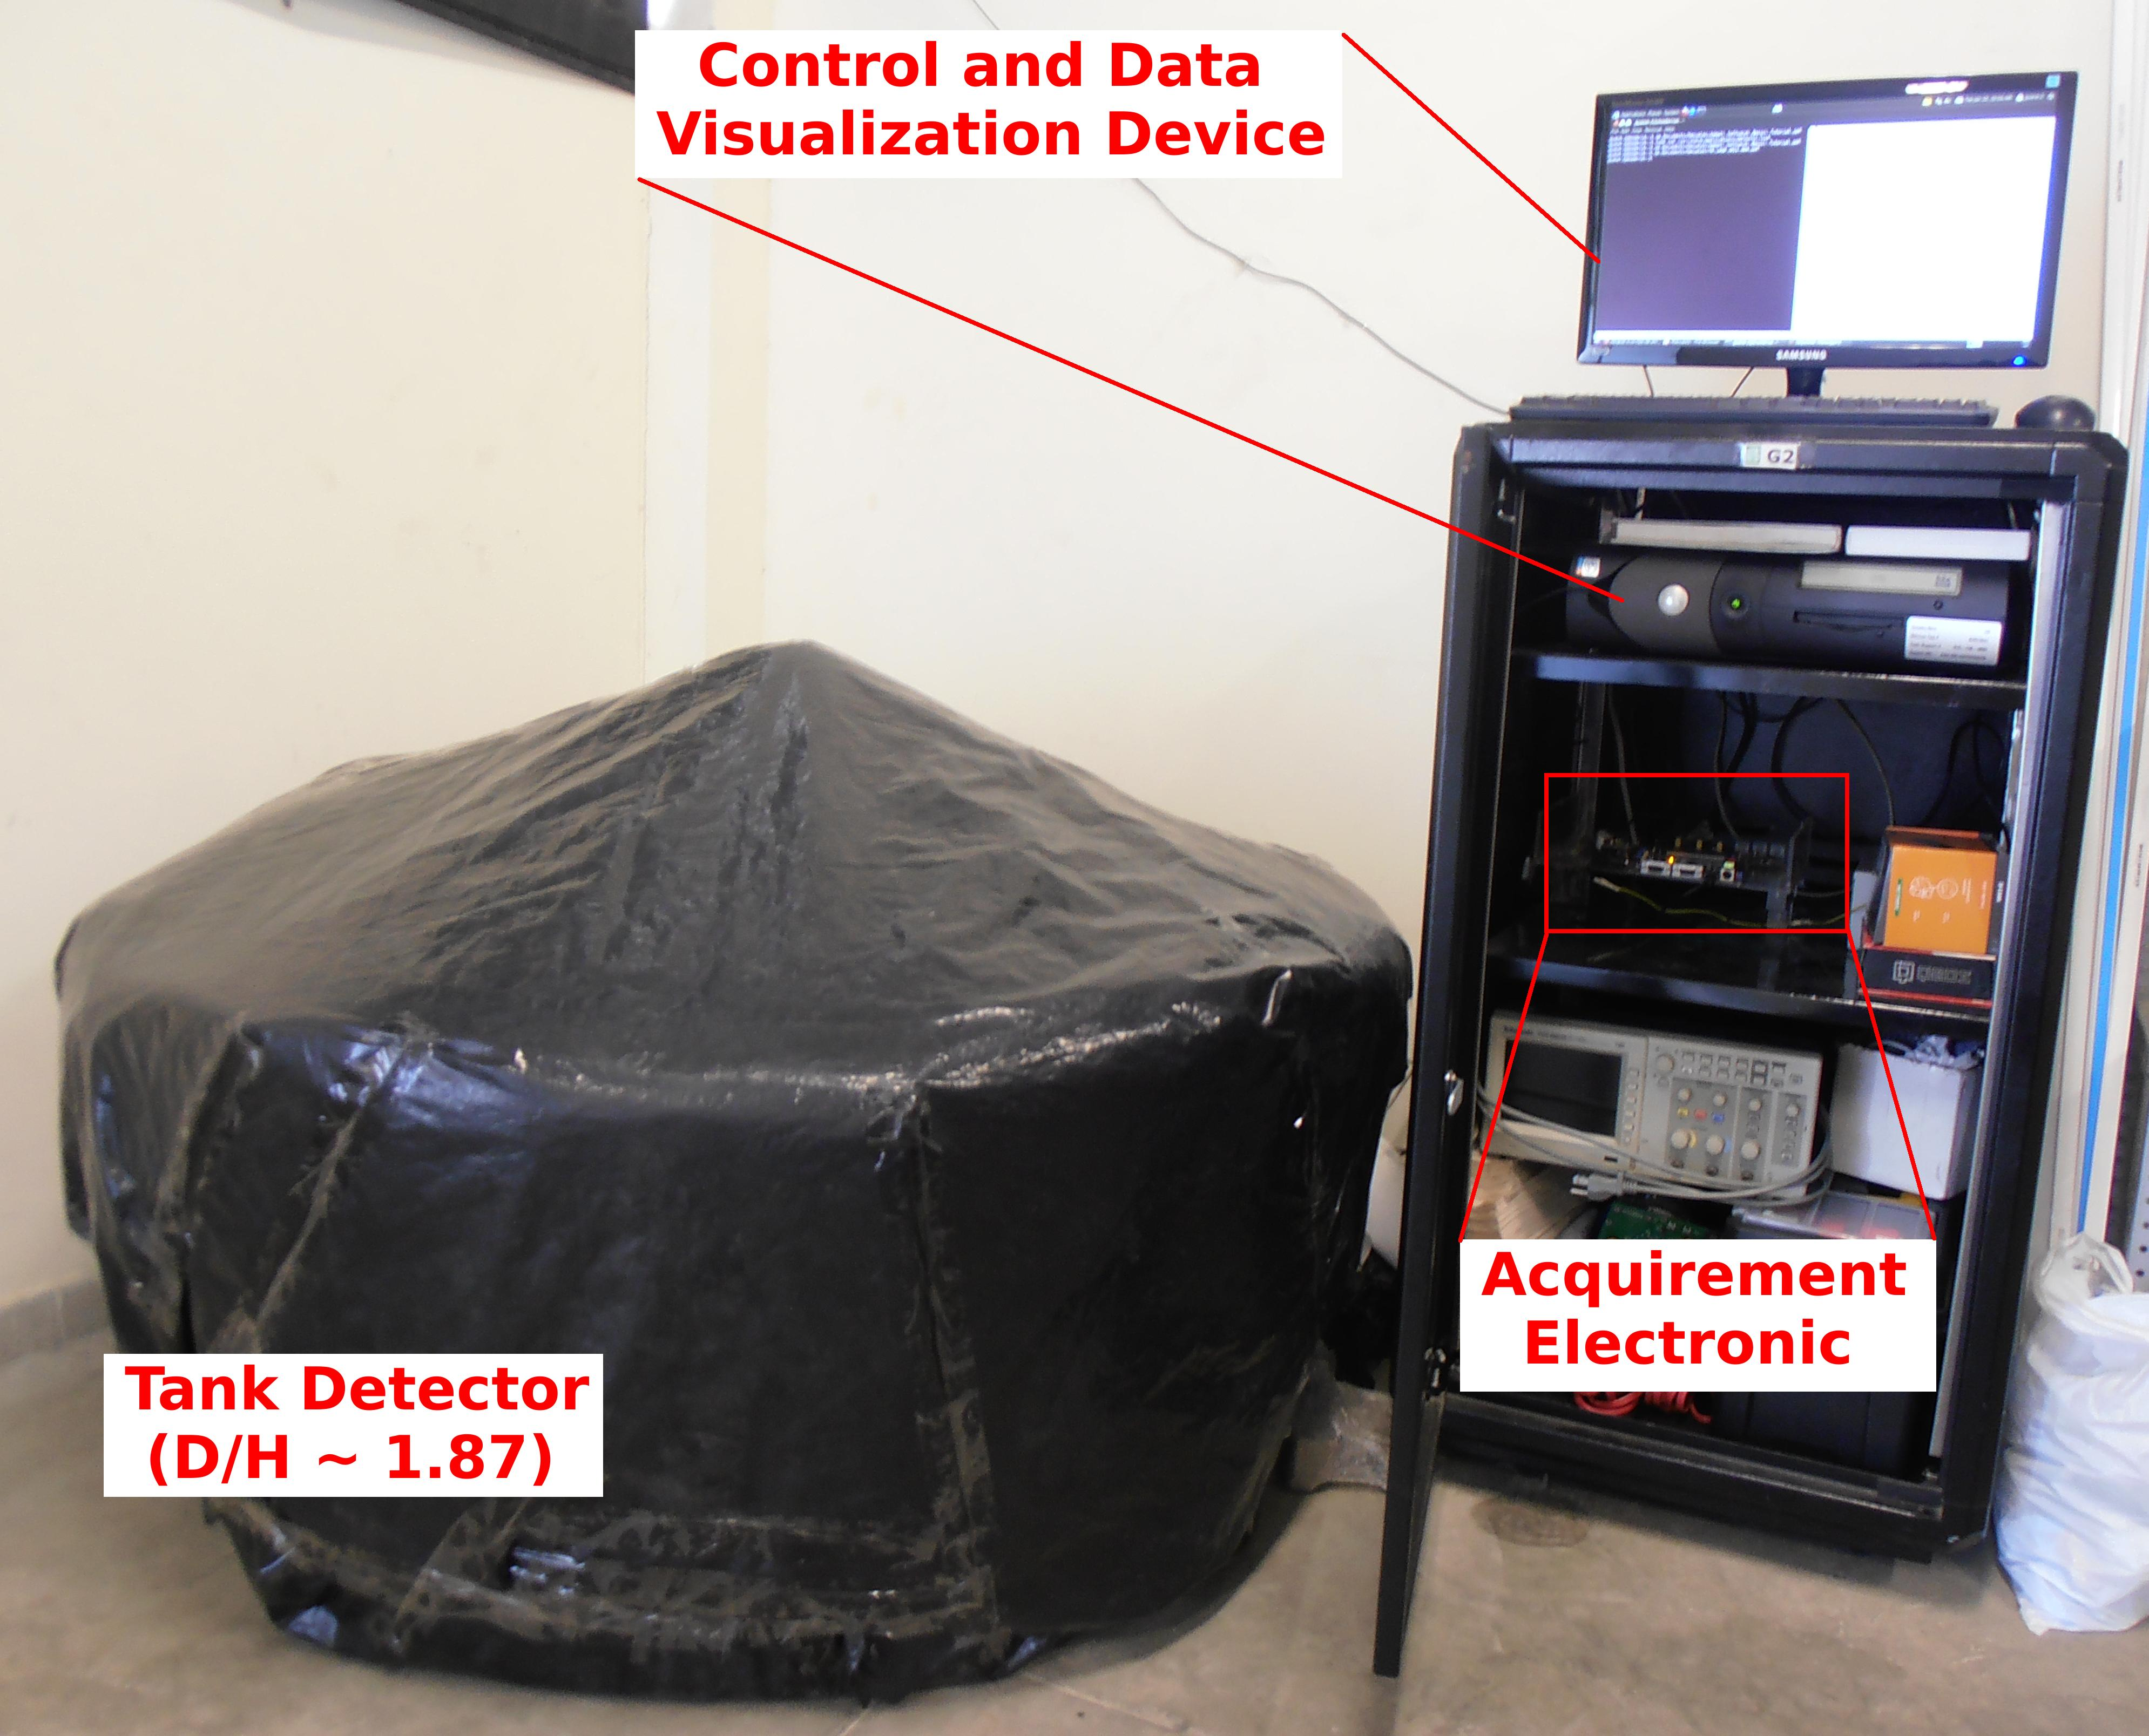
\includegraphics[width=3in]{images/colombia/WCD-Guane3.jpg}
\caption{GUANE-3 WCD at Bucaramanga.}
\label{fig:Guane3WCD}
\end{center}
\end{figure}

From fig. \ref{fig:results-col}, right, can be appretiated pulses registered by
Guane-3 having a particular shape: rapid increase and declining exponentially.

\begin{figure}
\centering
%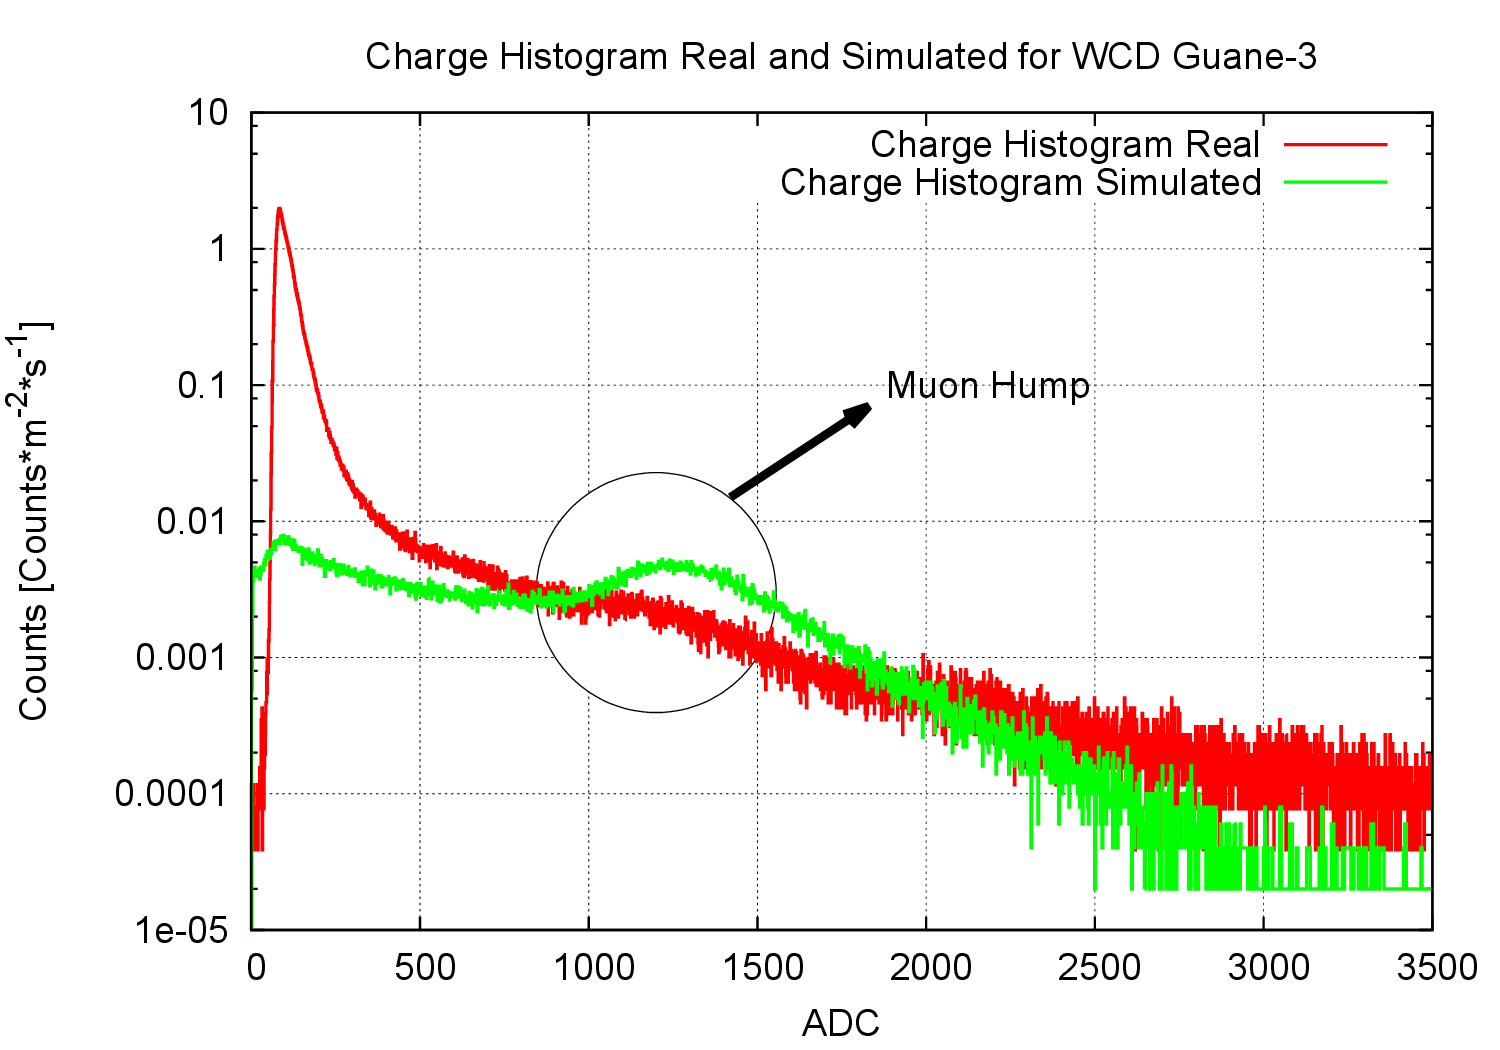
\includegraphics[width=0.49\textwidth]{images/colombia/Histcharge-Guane3.png}
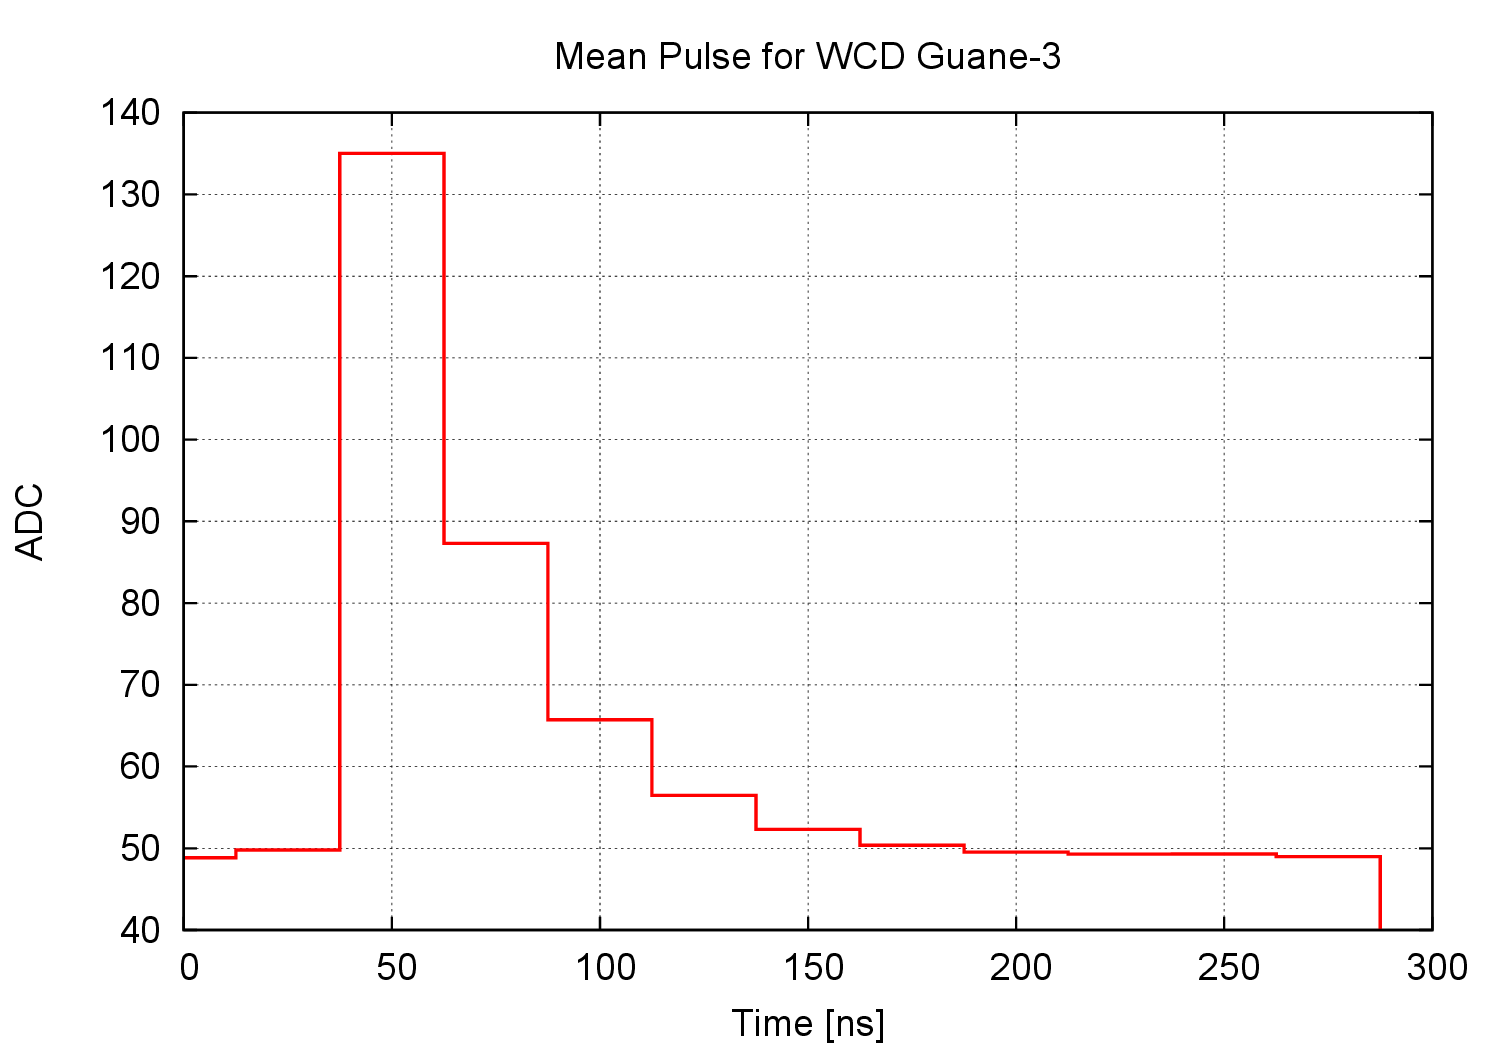
\includegraphics[width=0.49\textwidth]{images/colombia/MeanPulse-Guane3.png} 
\caption{Left: simulated and real charge histogram for the GUANE-3 WCD. Right: a plot of the mean pulse is depicted.} 
\label{fig:results-col}
\end{figure}

Calibrating, operating and monitoring WCDs at high altitude or remote
countryside places can be a significant complex task. The characteristic hump
left by muons in a WCD (such as the one used for calibrating the Pierre Auger
Observatory WCDs, see \cite{Bertou2006} is smeared by the large background
of electrons, positrons and photons. In order to calibrate Guane-3 WCD, it is
standard to use the VEM \cite{Etchegoyen2005}. Thus this unit defines the
high energy region ($>$1 VEM) and the low energy region ($<$1 VEM). The
equivalence between VEM and ADC units, can be obtained by comparing the charge
histograms with the corresponding Montecarlo simulations. For our Guane-3 WCD
we have 1 VEM $\sim 1200$ ADC. 


%seria bueno poner un grafico de esta calibracion!

   %4
\subsection{Ecuador}\label{subsec:ecu}

The WCD prototype ``Chimbito'' was installed in August $2012$ at Escuela
Polit\'{e}cnica del Chimborazo (ESPOCH) at $2870$~m a.s.l, which is about $60\
{\rm km}$ from the Chimborazo volcano.

\subsection*{Detector Prototype}

We use a commercial water tank, with a capacity of about 1100 l, and low
cost accessories to build the detector system. From bottom to top, the tank is
mostly cylindrical, followed by a truncated-cone section and a cylindrical end
at the top. The radius of the base of the main cylinder is 55\,cm, and its
height 110\,cm. The upper cylindrical part, which hosts the water tank cap, has
a diameter of 50\,cm and a height of 11\,cm. A detailed drawing can be seen in
Fig. \ref{fig:ecuador-tank}, left.

\begin{figure}[!ht]
  \centering
 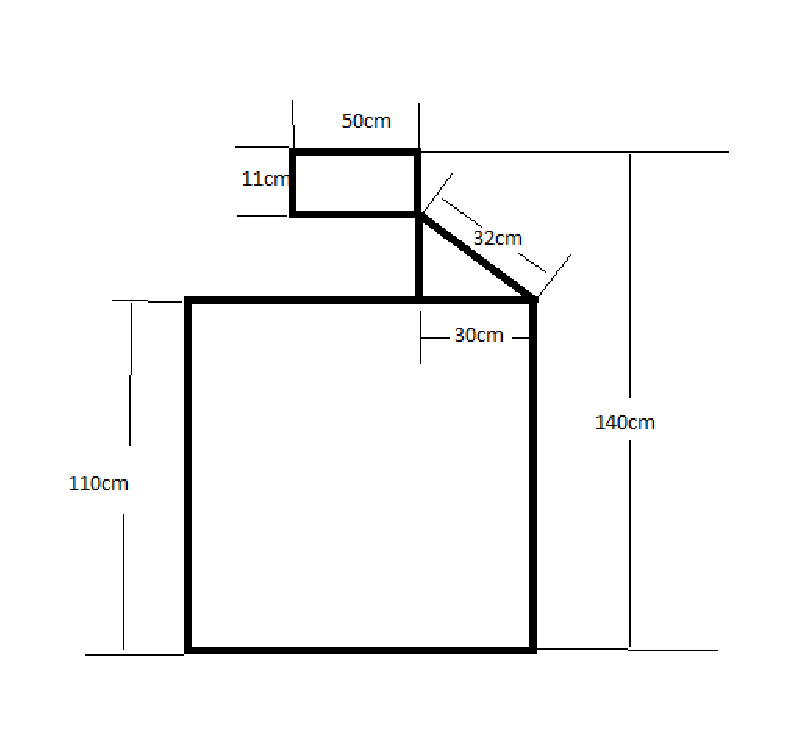
\includegraphics[width=0.45\textwidth]{images/ecuador/chimbito_dimensiones}
 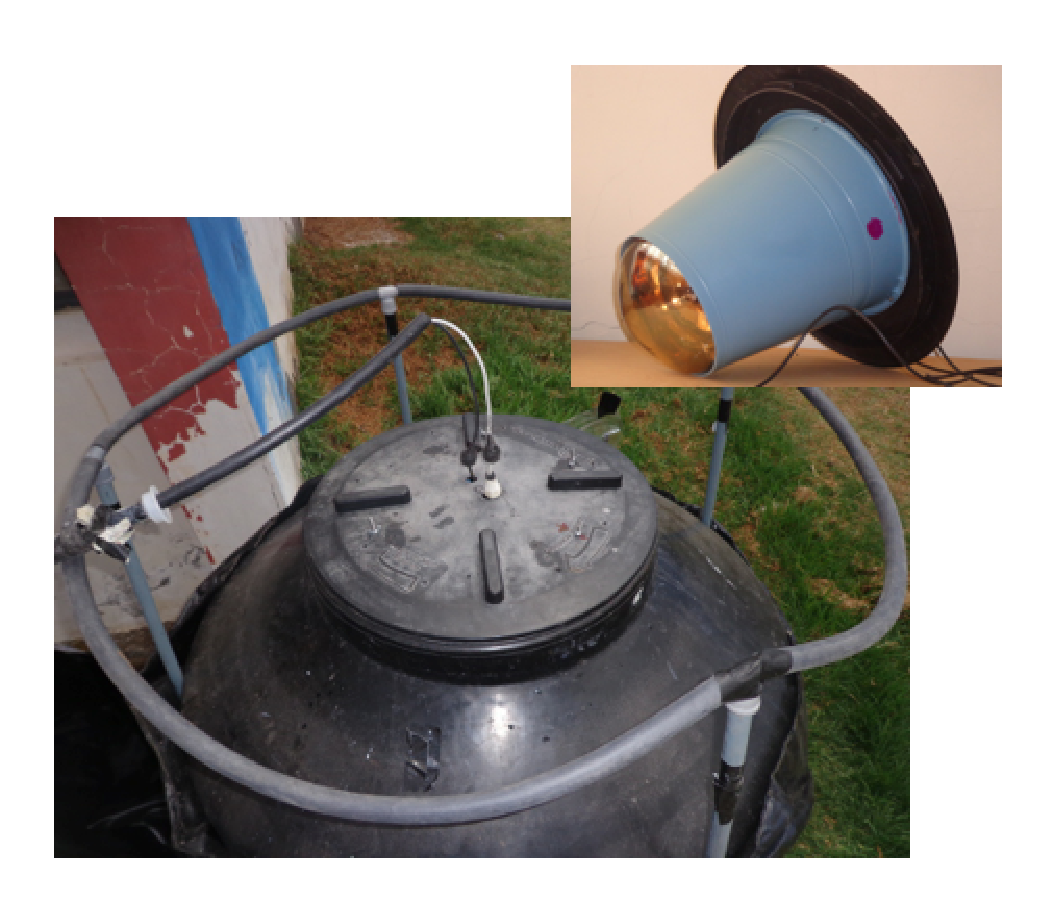
\includegraphics[width=0.45\textwidth]{images/ecuador/icrc2013-1208-01}
  \caption{Left: Dimensions of the WCD. Right: WCD prototype ``Chimbito'' installed at Riobamba, Ecuador. The PMT and its support are shown in the inset.}
  \label{fig:ecuador-tank}
 \end{figure}

The external walls of the tank are protected with four layers of high-density
non reflective black polyethylene. To guarantee good reflectivity and
diffusivity, the internal walls of the tank are lined with Banner-type
material. We also use Tyvek$^{\textregistered}$ as inner lining material
supported by a frame inside the tank and floating on top of the water. A
Photonis XP1802 9'' PMT is mounted for the Cherenkov light collection and
is placed at the top and central part of the detector cap. A hole was cut on
the Tyvek$^{\textregistered}$ surface in order for the PMT to protrude into the
inner part of the tank. The PMT is connected to a digitizer board and a FPGA,
whose connection was developed by the Bariloche group. The prototype is shown
in Fig. \ref{fig:ecuador-tank}, right. Special care has been taken to isolate this device
and its electronics board from moisture and to avoid water entering the PMT
hose. 

The shock chlorination technique has been used to improve the quality and
purity of the water. This process consists of the dilution of a high
concentration of chlorine Cl$_{2}$ into the water (approximately 150 mg of
Cl$_{2}$ per liter) in order to purify it. This method allows very low light
absorbance in a spectral range from $350$ to $750$\,nm. However, due to its low
cost and relatively easy way to apply, it has been chosen as the default method
of purification. It is important to mention that it is the first time that this
process is used to purify water for WCD in the LAGO Collaboration. Furthermore,
Amino-G, ${NH_{2}C_{10}H_{5}(SO_{3}H)S)_{3}Na}$, the most common wavelength
shifter used in water Cherenkov detectors, has been added to the water in a
concentration of $1$\,mg per liter. Studies report that, with this addition,
the efficiency of the detector increases by a factor of 3 without loosing the
directionality of Cherenkov light \cite{Badino1981}.

\subsection*{Operational Status of the Detector}

In the top panel of figure \ref{fig:results-ecu}, it is shown an individual
pulse and the mean signal response of the detector for data taken in September
2013.

 \begin{figure}[!ht]
  \centering
 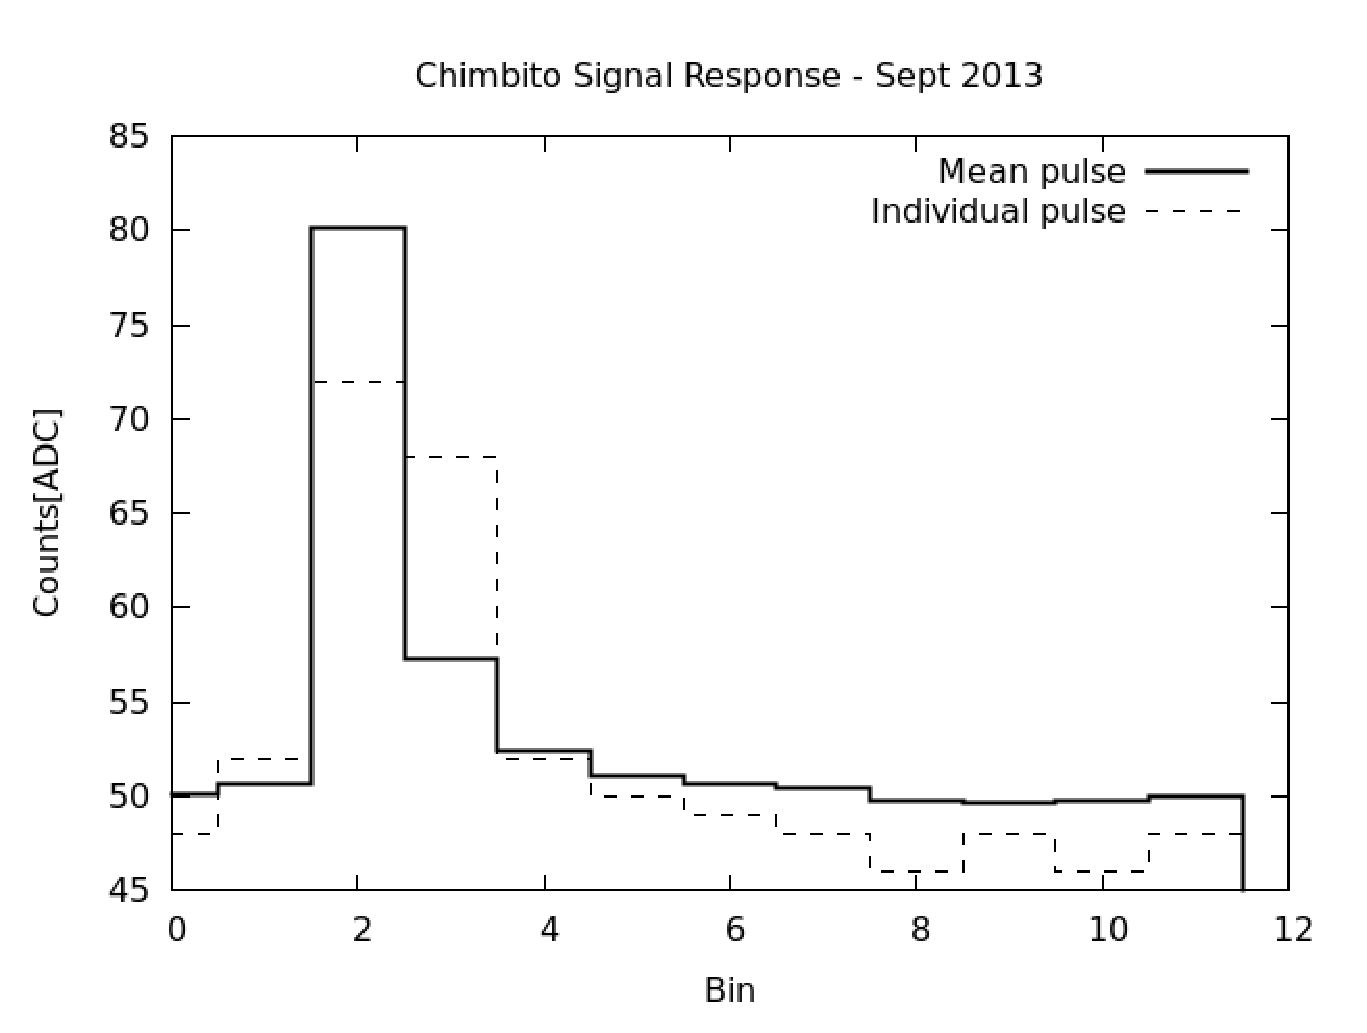
\includegraphics[width=0.8\textwidth]{images/ecuador/promedioSep21h}
 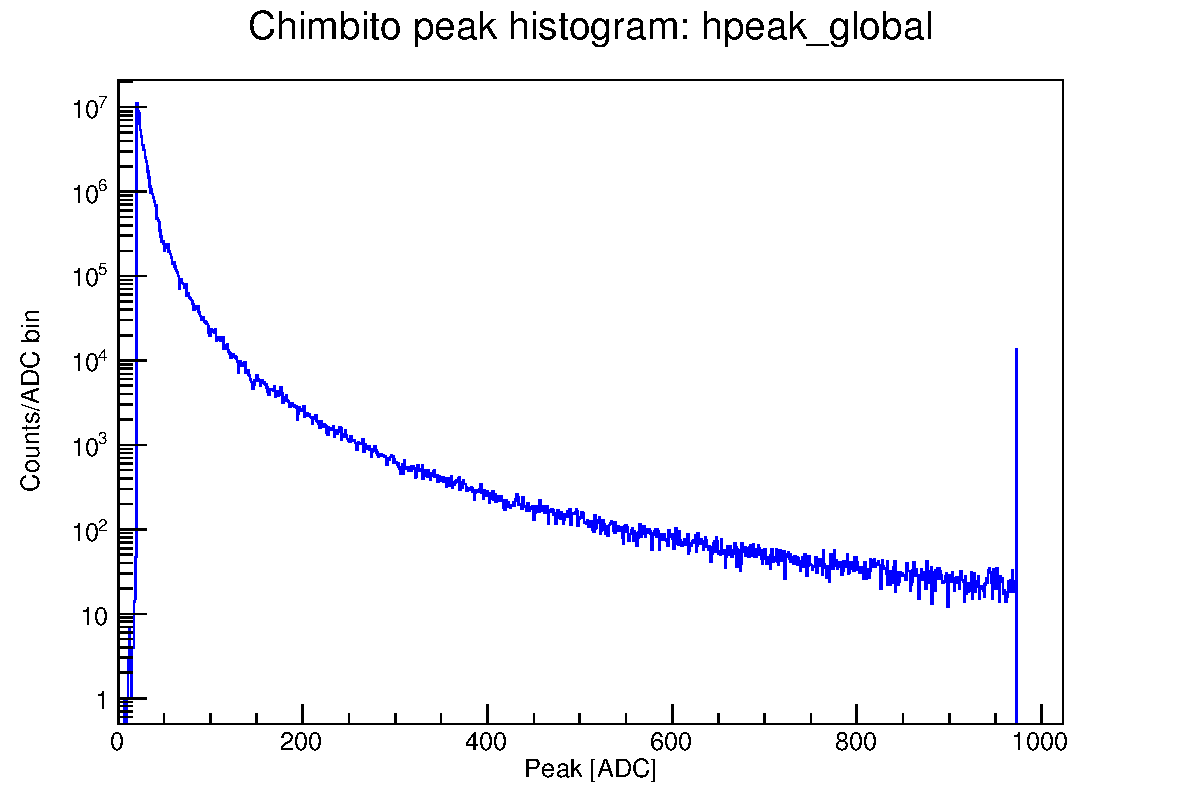
\includegraphics[width=0.49\textwidth]{images/ecuador/peak_histo_chimbito_jul_nov_2013}
 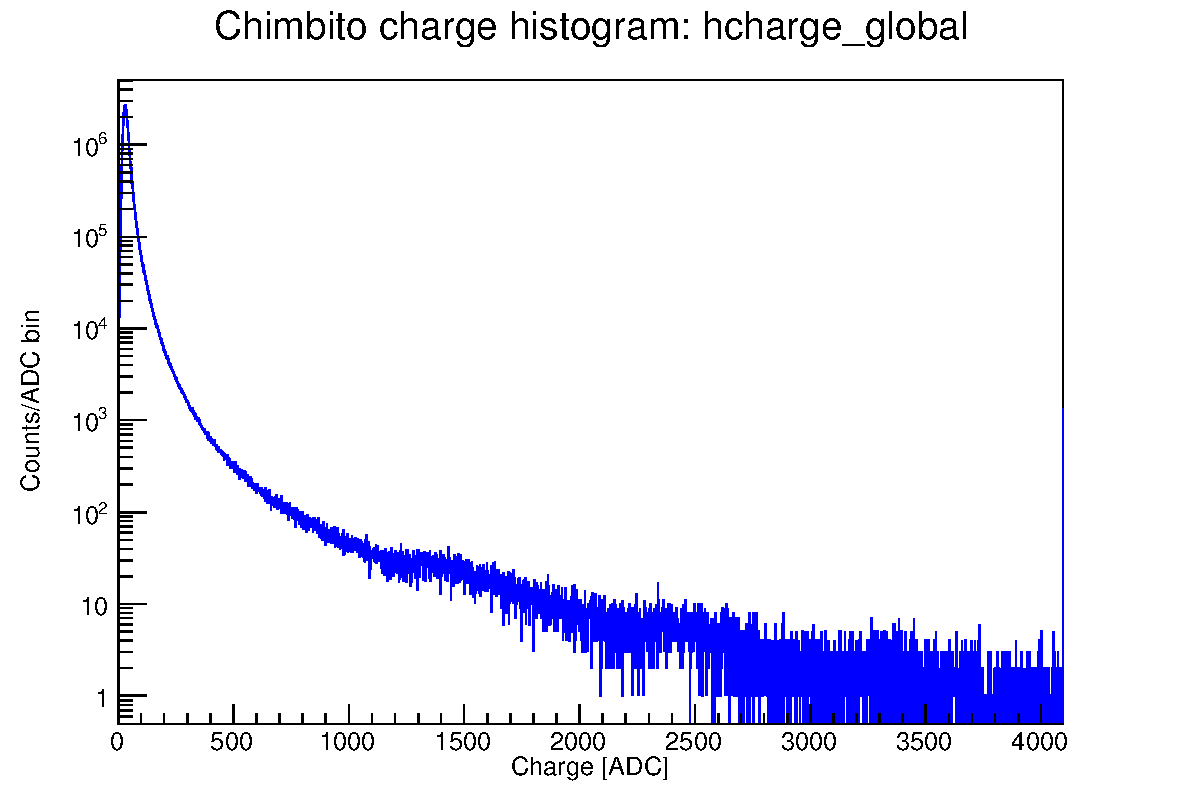
\includegraphics[width=0.49\textwidth]{images/ecuador/charge_histo_chimbito_jul_nov_2013}
  \caption{Top: mean signal response ``Chimbito''. The individual signal response of a pulse is also shown. Bottom left: Peak histogram with data taken between July and November 2013. Bottom right: charge histogram with data taken between July and November 2013.}
  \label{fig:results-ecu}
 \end{figure}

Calibration histograms have been extracted from the collected data. A total
charge histogram and a peak histogram for data collected between July and
November of $2013$ are shown in bottom right panel and bottom left panel of
figure \ref{fig:results-ecu}, respectively. 

Currently, all the flowing data is being analyzed and interpreted in order to
understand the performance of the detector and to identify any possible changes to
the hardware configuration. The calibration of the detector using the muon peak
is expected to be done in a short time.

In the near future, the final objective is to locate a new detector in the
Chimborazo snowcap foothills at 4800 m a.s.l., which will be, to our
knowledge, the second highest LAGO site after Chacaltaya (see table \ref{tab:locations}),
Bolivia. The data taken from this new detector is expected to be compared with
the data obtained with the ``Chimbito'' detector. Due to the high altitude of
this site  this comparison could increase the detection sensitivity of
transient events emitting high energy photons.

It is worth mentioning that a new WCD prototype ``Panchito'' is under
construction at Cumbaya, Quito (2398 m a.s.l.), Ecuador. This detector will be
located at Universidad San Francisco de Quito (USFQ). We will use a commercial
water tank of 2500 l similar to the one used in ``Chimbito'' design but with a
geometry better suited for photon detection. The radius of the base of the main
cylinder is 78.4\,cm, and its height 146\,cm. The upper cylindrical cap has a
diameter of 55\,cm. The internal walls of the WCD will be covered by
Tyvek$^{\textregistered}$ and Banner-type material in a manner similar to the
detector in Riobamba. The PMT XP1802 9''produced by Photonis will be connected
to an acquisition board. It has sensitivity over a wide spectral range, from
270 to 650\,nm.

A new high altitude site near the east side of Pichincha Volcano, Cruz Loma at
4100 m a.s.l., is also under consideration. This detector is expected to be used
for high energy physics analysis. Meanwhile, ``Chimbito'' and ``Panchito''
detectors will be used for solar physics analysis and software development.
Multiple comparisons could be done using the data obtained with this detector
array.
    %5
\subsection{Guatemala}\label{subsec:gua}

In Guatemala the site is located at the top of the roof of the T1 building of
the University of San Carlos de Guatemala. The size of the detector is 1.2\,m
height, 1.12\,m wide and has a capacity of 1,100\,l. The inside is coated
with a reflective Flex polyvinyl chloride sheet and the PMT is a 9" photonis
XP1802.

The electronic of the detector is the original from the Bariloche groupand was
running from June 2011 until March 2012.


\begin{figure}[h]
\begin{center}
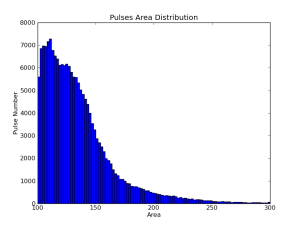
\includegraphics[width=0.48\textwidth]{images/guatemala/Histo.png}
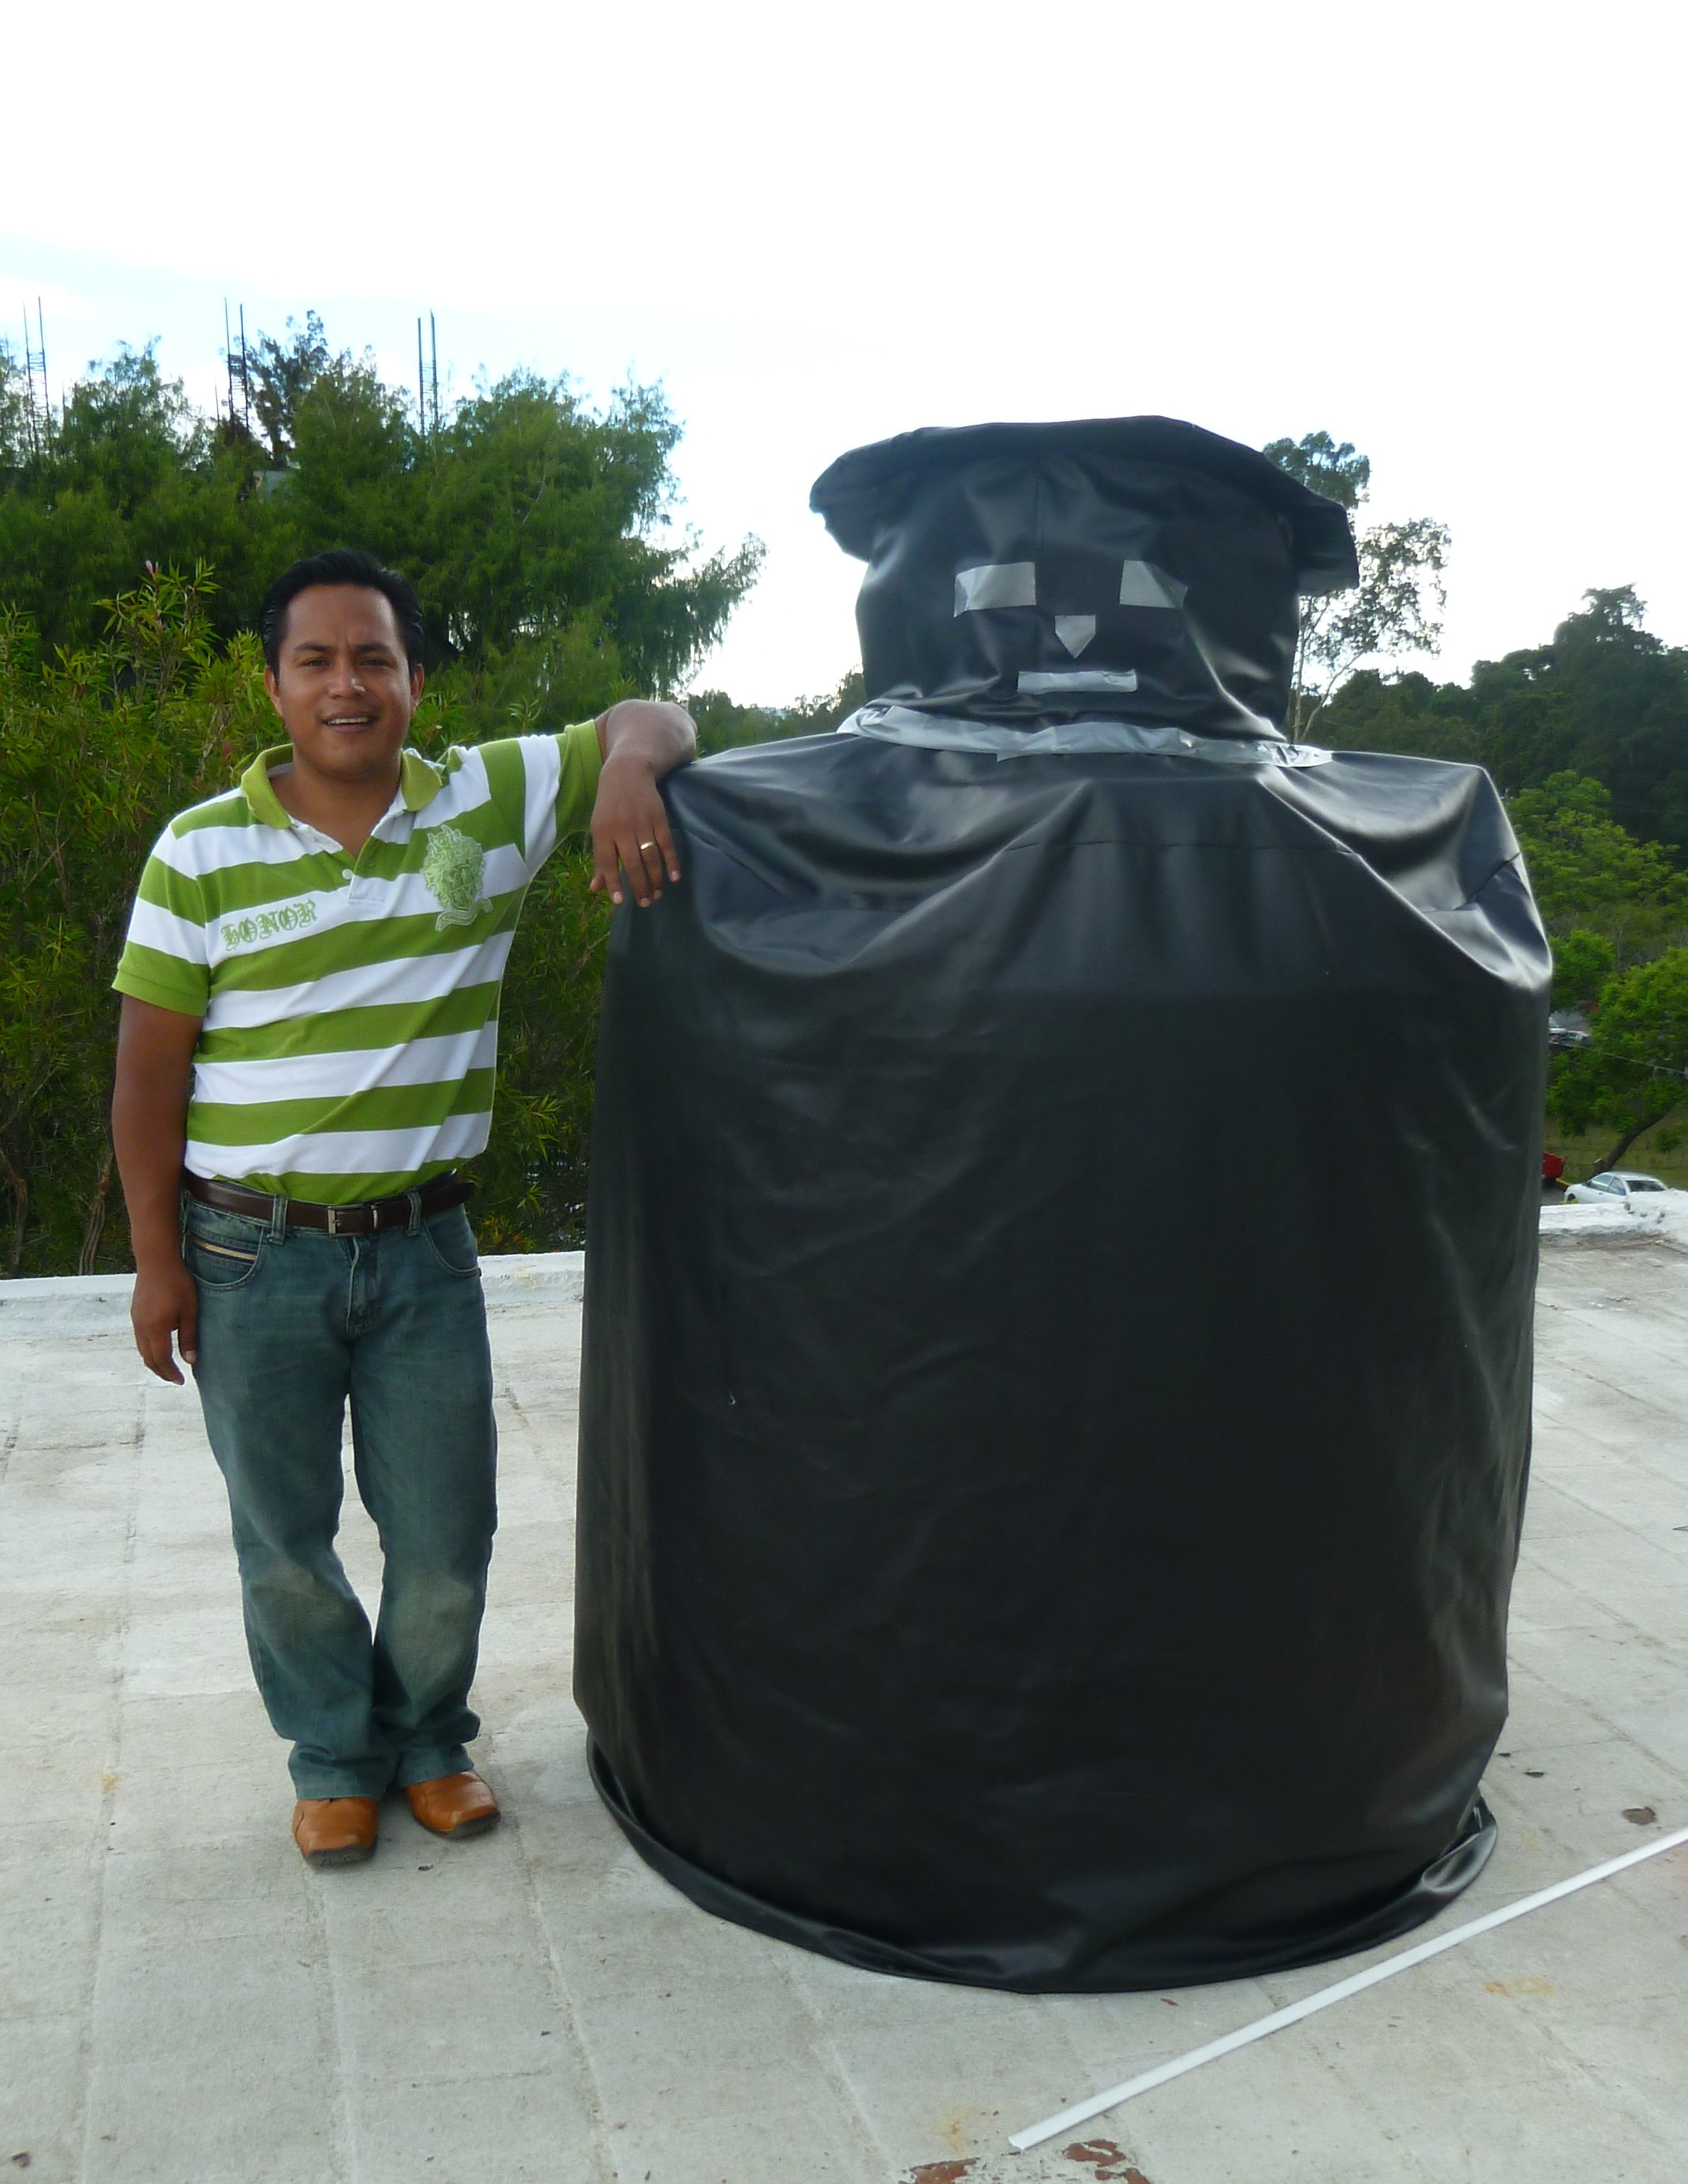
\includegraphics[width=0.48\textwidth]{images/guatemala/DimDet.jpg}
\caption{Histogram of an event of the uncalibrated detector. The area is proportional to the charge recolected. The second peak corresponds to a muonic trace.The entire detector is covered with black semi-leather.}
\label{fig:Histo-guate} 
\end{center}
\end{figure}
  %6
\subsection{M\'exico}\label{subsec:mex}

\subsubsection*{Detector description}

Sierra Negra is the first LAGO site with WCD working (since early 2007). Until
2010, 3$\times$4\,m$^{2}$ area Cherenkov detectors, in a 30\,m triangular array
were taking data at this site each detector had an EMI 9030A photomultiplier
tube, looking towards the bottom. The output of the phototube was connected to
a data acquisition card used in the development of this phase.

\subsection*{Upgrade of the SN LAGO set up}

The Sierra Negra site of the LAGO experiment has four detector of 40\,m$^{2}$,
three of them located at the vertex of an equilateral triangle of 30\,m. 
Those detectors are cylindrical tanks, made with a corrugated steel plated
bolted with stainless steel screws, 7.3\,m of diameter and 1.15\,m high. The
tops and inside of each detector are covered by an EPDM (Ethylene Propylene
Diene Monomer) black liner to contain and protect the radiator media.
The EPDM material is elastic, easy to weld and mechanically very strong,
helping to have a light tight and insulated inner environment. The body and
the bottom of the detector are covered with a bag of high diffusive and
reflective material: white polyethylene banner. The white bag is filled with
high quality purified water up to a level of 1.1\,m and in the upper surface;
there is a Tyvek sheet floating in order to reflect the Cherenkov light
produced as uniformly as possible. The special feature of this kind of Water
Cherenkov Detector is its inner segmentation. To improve the light collection,
we have installed reflective walls with the same material that the inner liner,
The cylinder was divided at four regular sectors; one hemispherical 8" diameter
PMT located in the centroid of each one, looking downwards, The PMT
photocathode is submerged to avoid losses by any air-water interface. The
entire container is covered and protected externally by a black, light-tight
bag and a canvas roof. The Cherenkov light is collected by the electron
phototube 9354KB of Electron Tubes Ltd., installed up towards the bottom.

\begin{figure}[th!]
\centering
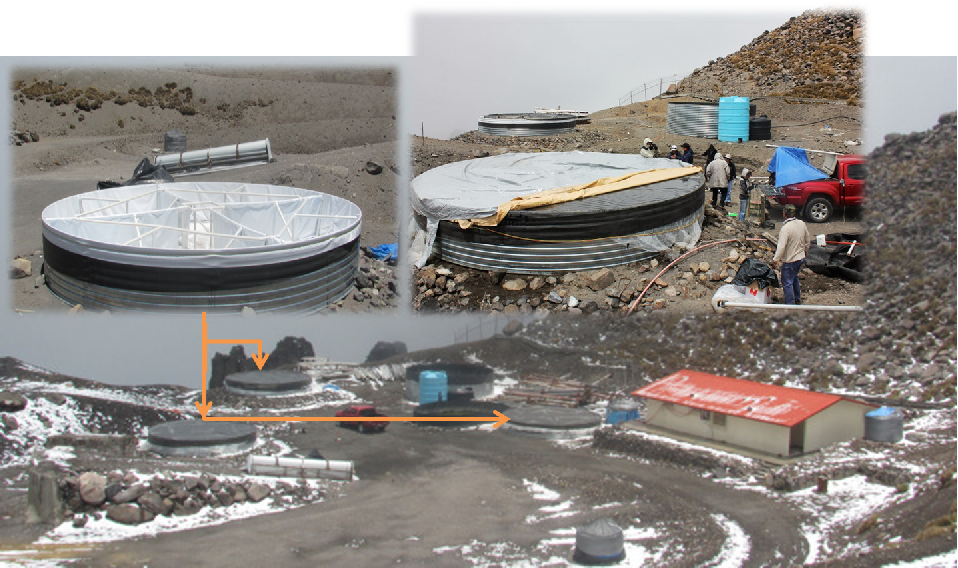
\includegraphics[width=0.8\textwidth]{images/mexico/sitelago-01.png}
\caption{LAGO Sierra Negra WCDs. An old array of small tanks is clearly seen
between the new big stainless steel tanks.  Those are covered by a black EPDM
liner. B.- Internal structure of the new WCD. The structure of the PVC pipes
allows us to set the banner walls to divide it into four sectors and fix the
PMT and cables in a safety way. Also help us to keep 
the upper liner and a canvas roof.}
\label{sitelago01}
\end{figure} 

At the center of the array we will set a WCD with the same area, but 4.5\,m height, 
filled with clean water and 4 PMT at the bottom looking upwards. This detector
has the aim to reject hadrons when a extensive air shower is detected.

\subsection*{Operation and calibration of the WCD Detectors}

Calibration mode. It consists on the data acquisition of 32 consecutive samples
in 10 ns intervals (100\,MSPS\footnote{Mega Samples Per Second}) of the digital
pulses produced by an ultraviolet LED with wavelength of 405\,nm with a 15\,ns
wide pulse in a frequency of 10\,kHz located 60\,cm from the PMT. The phototube
polarization voltage and the LED polarization voltage are fine tuned. It
provides us with a minimal response that represents a fundamental part for the
calibration of a PMT.

As shown in figure \ref{sitelago04} and figure, \ref{sitelago05}, we can plot
the response to a single photo-electron using our DAQ (see section
\ref{sec:detector}). The curves correspond to high voltages of 1.25\,kV,
1.3\,kV, and 1.35\,kV. The best single photo-electron response, for this PMT,
is obtained at 1.3\,kV and this value was set as the operation one.

\begin{figure}[t]
\centering
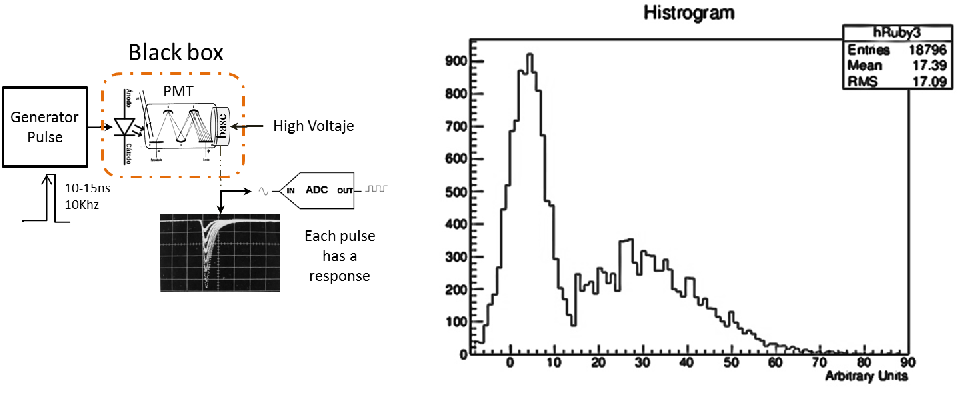
\includegraphics[scale=0.4]{images/mexico/sitelago-04.png}
\caption{Mode calibration and Response to a single photo-electron, using the new DAQ.}
\label{sitelago04}
\end{figure} 

\begin{figure}[t]
\centering
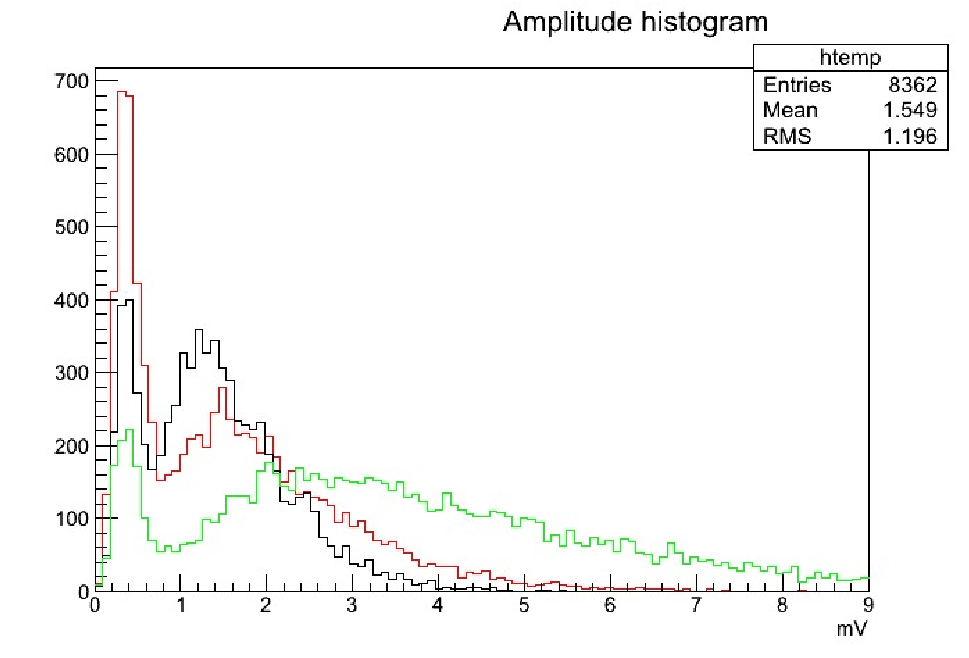
\includegraphics[scale=0.4]{images/mexico/sitelago-05.png}
\caption{Plot of the response to a single photo-electron by the PMT at 1.25\,kV (black), 1.3\,kV (red), and 1.35\,kV (green). The operation voltage was fixed at 1.3\,kV.}
\label{sitelago05}
\end{figure} 

%Examples of traces, baseline and threshold are shown in \ref{sitelago06}.
%
%\begin{figure}[t]
%\centering
%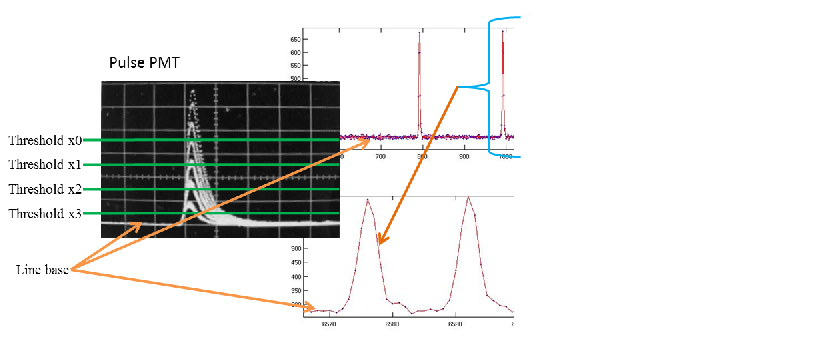
\includegraphics[scale=0.5]{images/mexico/sitelago-06.png}
%\caption{Example who shows the base line the trace and the rate.}
%\label{sitelago06}
%\end{figure} 
     %7
\subsection{Per\'u}\label{subsec:per}

In Lima there are two WCDs in operation, in the building of the National
Commission for Aerospace Research and Development (CONIDA). One in the roof and
one below, separated by a floor and concrete walls of 30 cm thick. The purpose
of this configuration is to operate them in telescope mode.

The detectors were made with small commercial tanks of polyethylene, the light
insulation is made of a number of layers of black polyethylene. Also the upper
tank has an extra plastic cover to protect the environment. The water used in
the detector has been filtered by a commercial water purifier that has filters
of 5 and 1 micron, an osmosis membrane filter and activated carbon filter.
A picture of the detector can be appretiated in fig. \ref{fig:peru-site}

The PMT used is the EMI9530A model, for operation there is a voltage divider
custom designed and a high voltage source. However, the signal left in the
detectors is small (see fig. \ref{fig:peru-res}) compared to the range in which
it is able to digitize the card so a stage of signal amplification is under
development.

\begin{figure}[h!]
\begin{center}
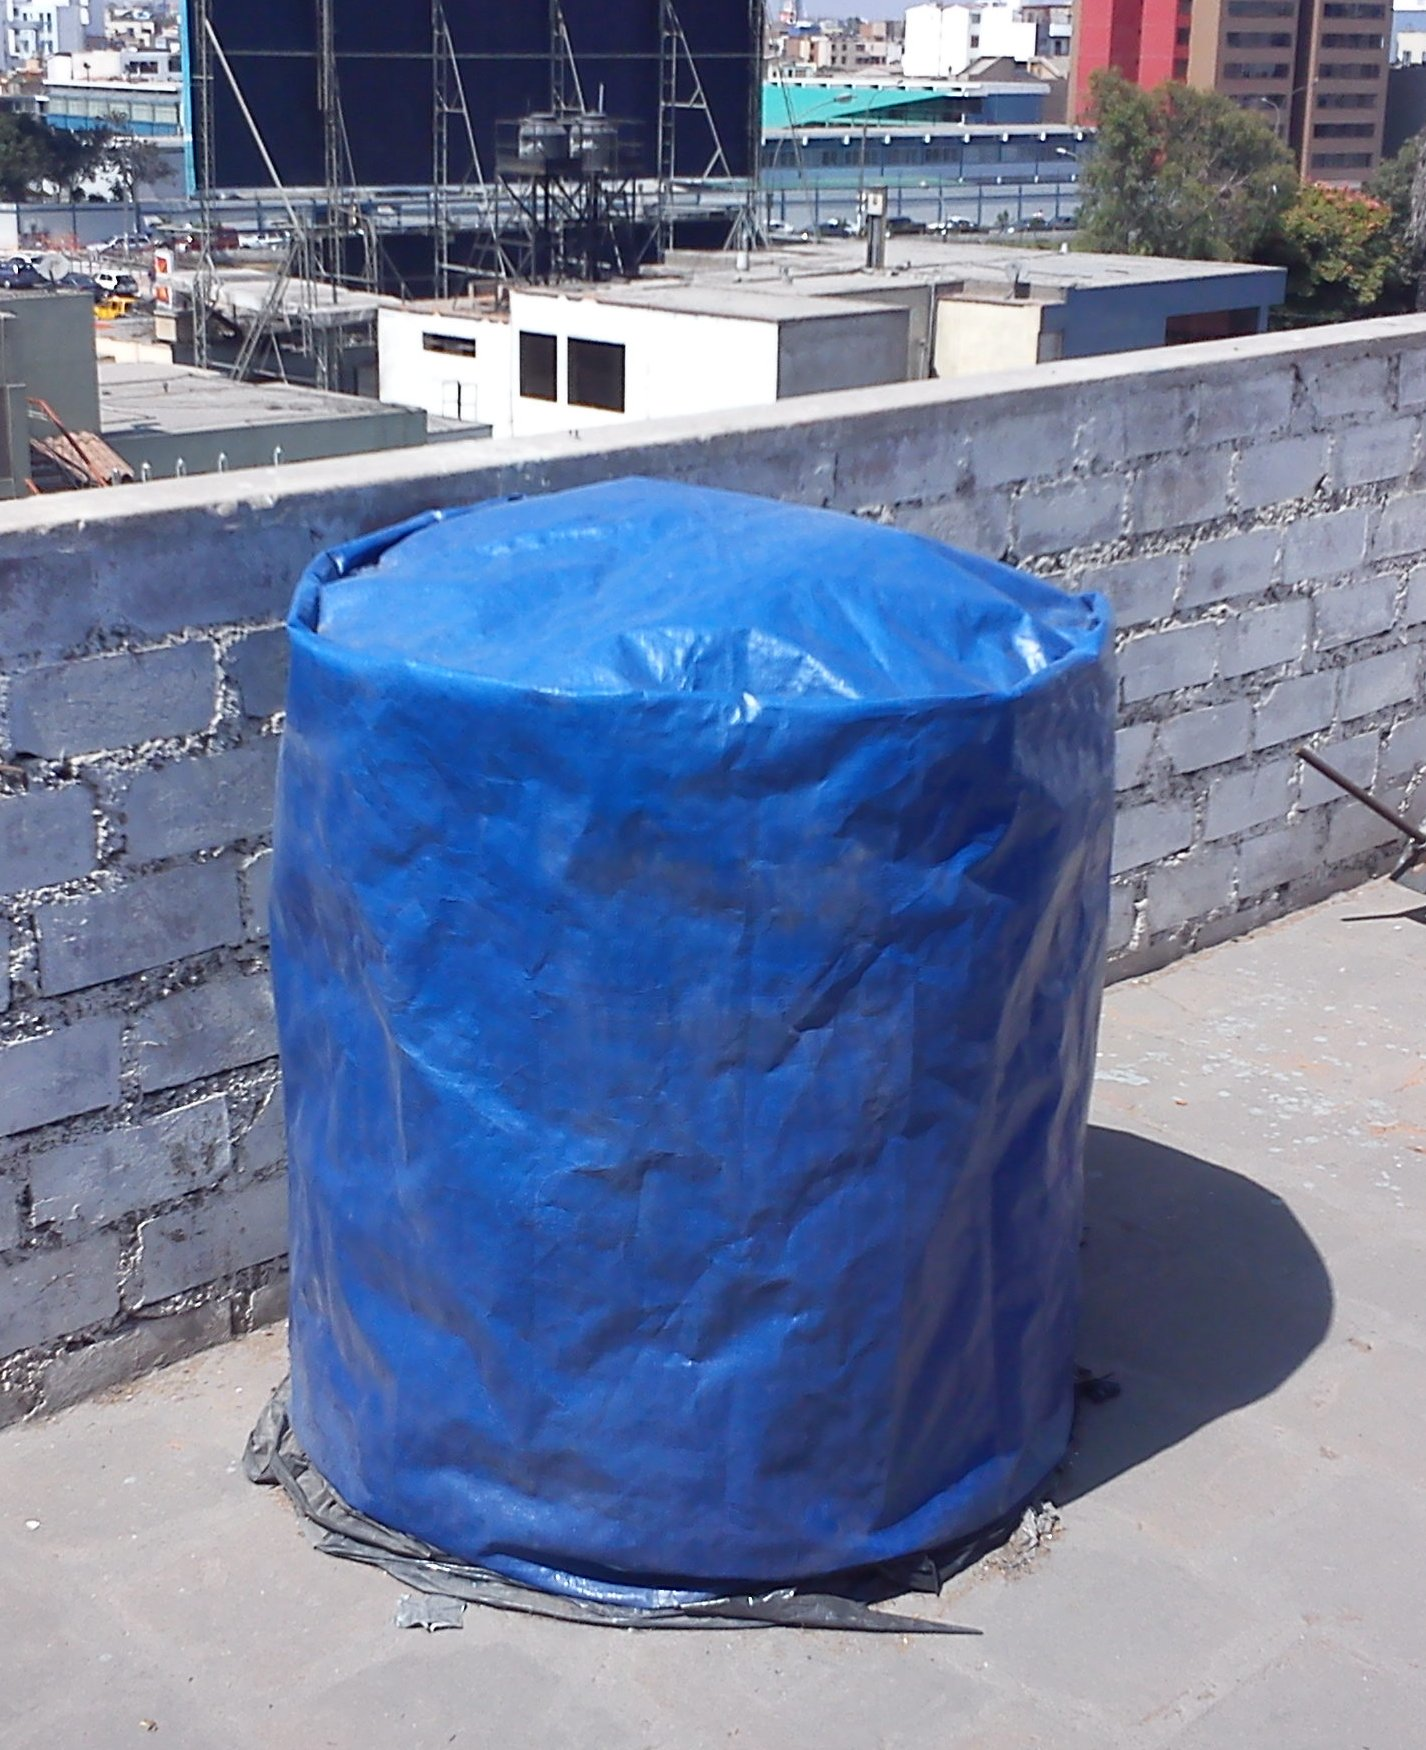
\includegraphics[width=0.40\textwidth]{images/peru/wcd.jpg}
\caption{WCD at the top of the roof in Lima.}
\label{fig:peru-site}
\end{center}
\end{figure}

At thirty minutes trip from the city of Huancayo in the Geomagnetic Observatory
Huayao is still in testing a new WCD design, similar to those developed by
Lago-Mexico but smaller. It is constructed with a steel cylindrical side
surface of 3\,m of diameter and 1\,m high, which supports the volume of water
in a cylindrical black polyethylene bag. The inner reflector material is banner
and has some PVC tubes that maintain the shape of the plastic bags and hold the
PMT, an ET9354KB. The water of the detector has been treated by a process of
flocculation and sedimentation with aluminum sulfate (procedure recommended by
LAGO-Venezuela).

\begin{figure}[h!]
\begin{center}
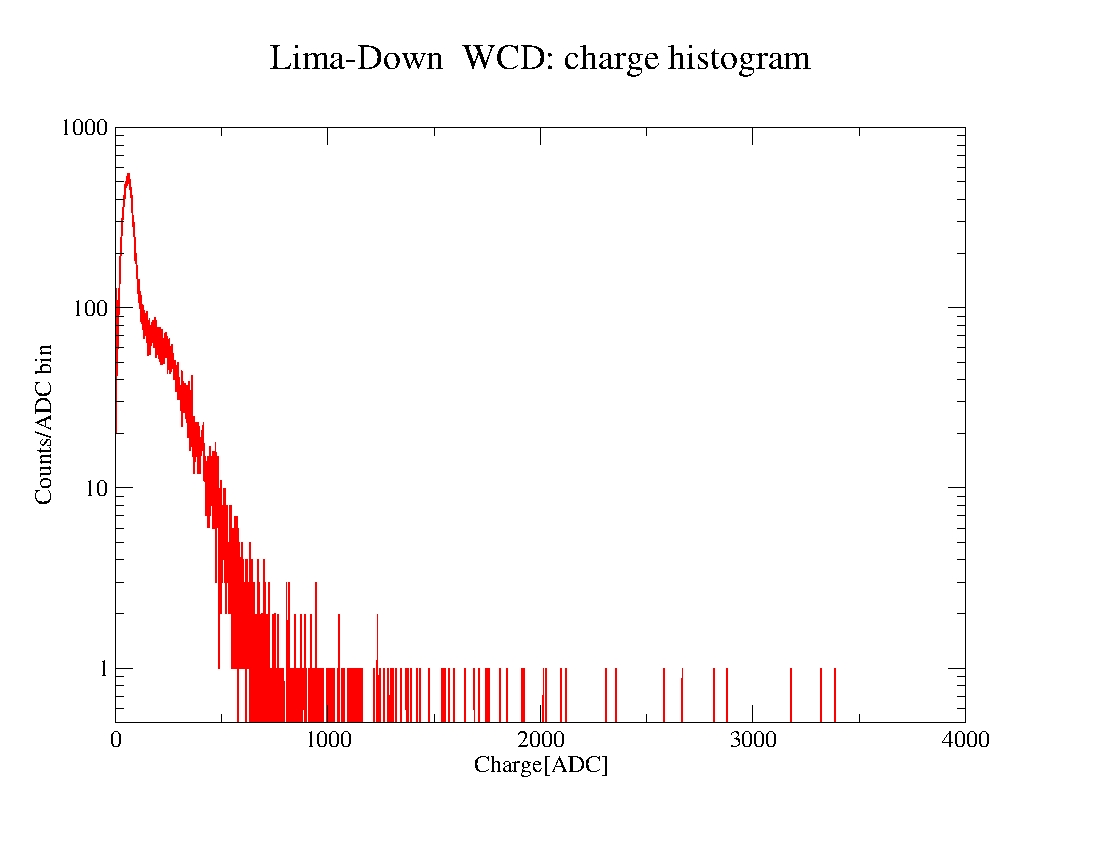
\includegraphics[width=0.49\textwidth]{images/peru/Lima_down_charge.jpg}
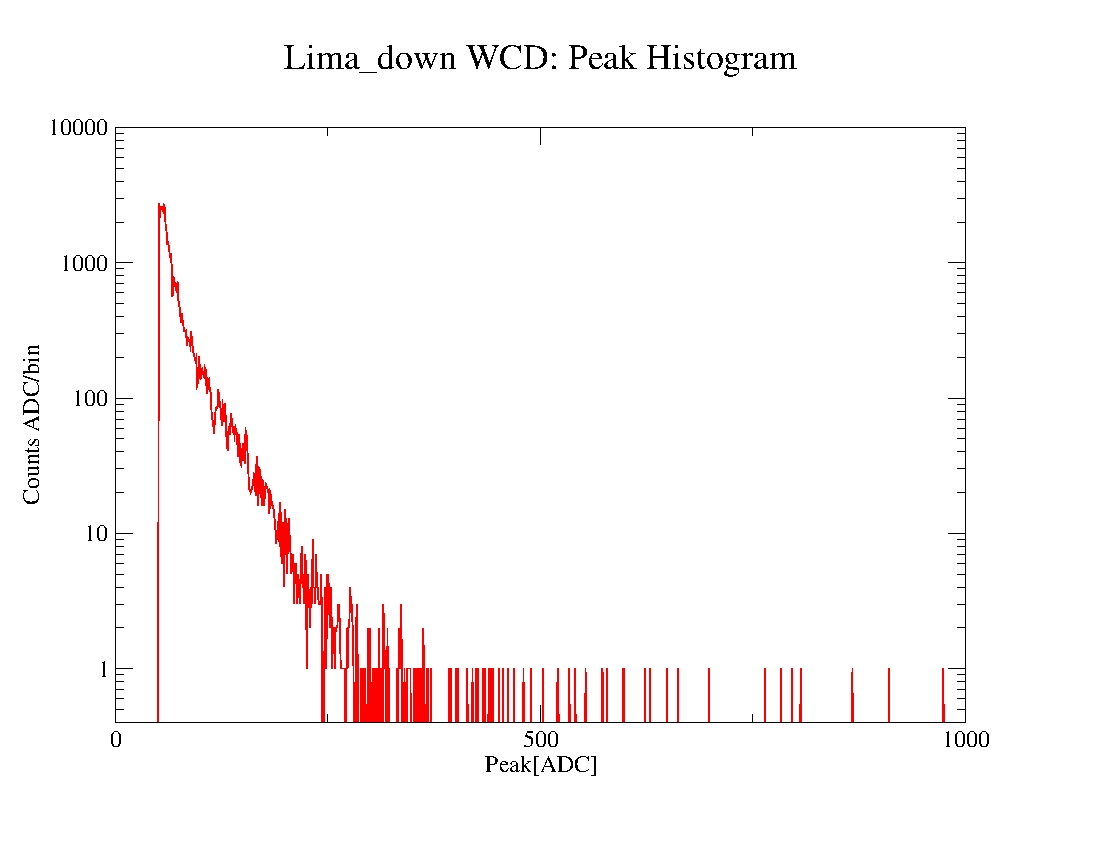
\includegraphics[width=0.49\textwidth]{images/peru/Lima_down_peak.jpg}
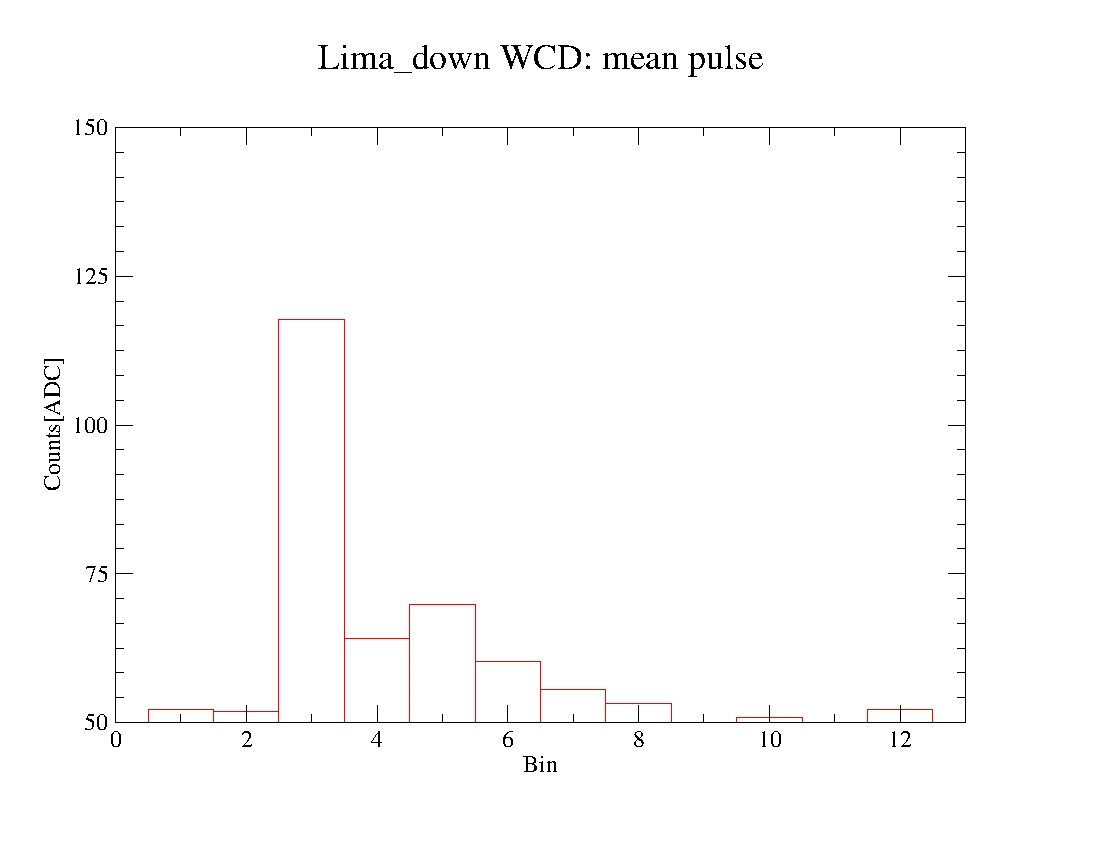
\includegraphics[width=0.5\textwidth]{images/peru/lima_down_pulse.jpg}
\caption{Top left: Histogram of charge from one of the WCD in Lima. Top right: histogram of pulses of the same WCD. Bottom: one hour pulse average.}
\label{fig:peru-res}
\end{center}
\end{figure}

\begin{figure}[h!]
\begin{center}
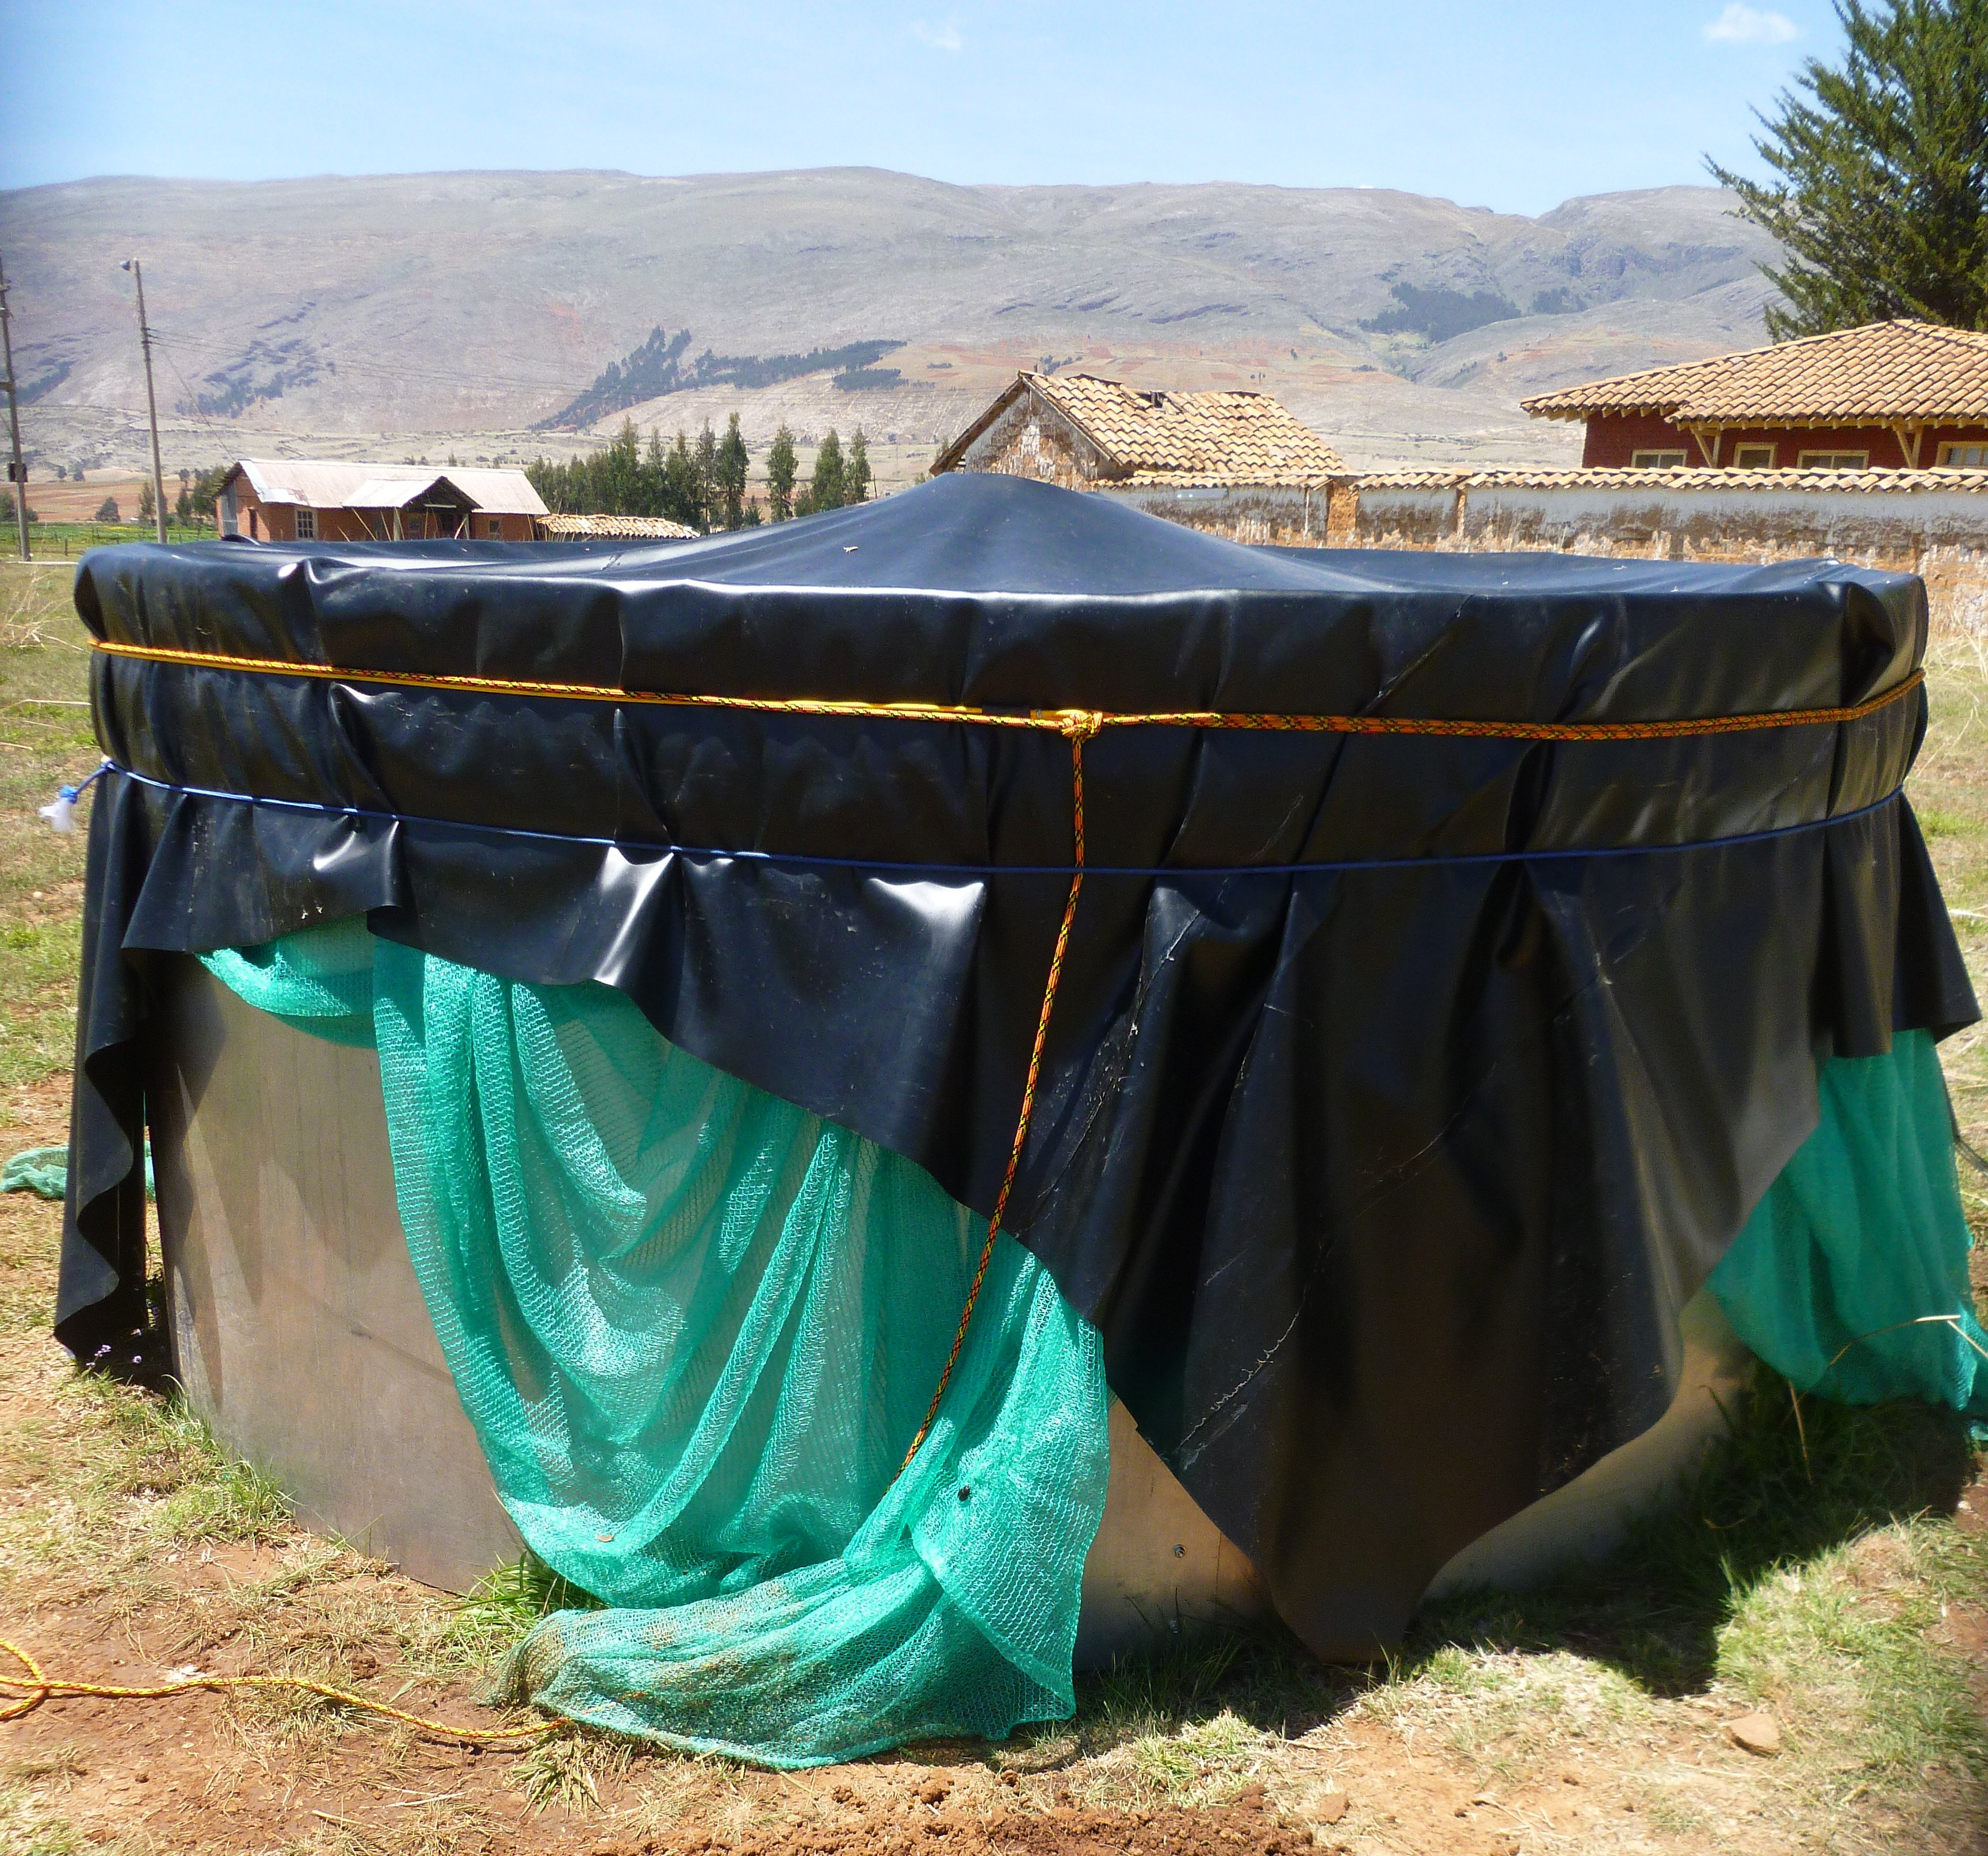
\includegraphics[width=0.47\textwidth]{images/peru/WCD_Huancayo.JPG}
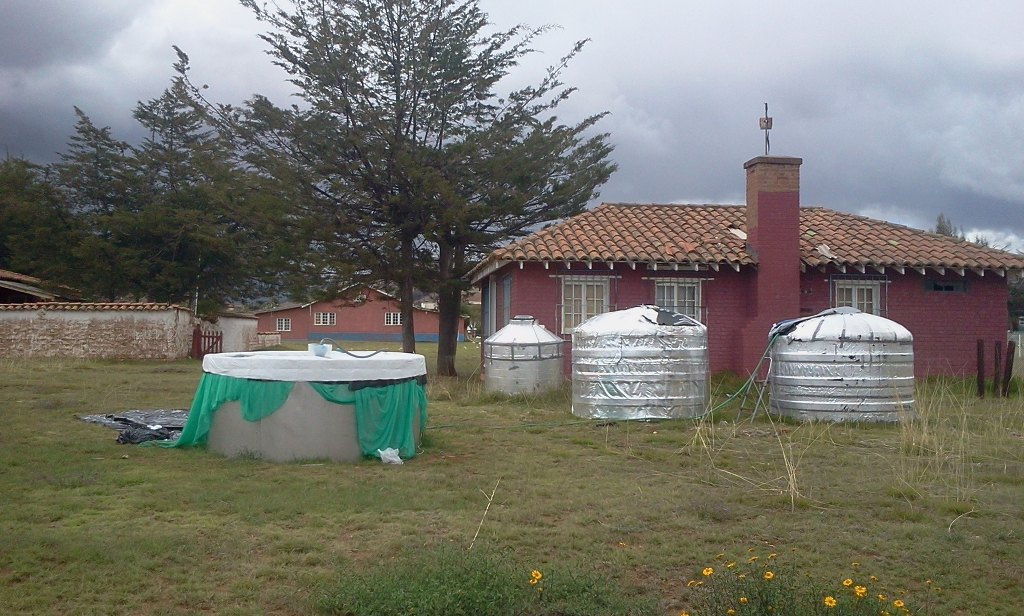
\includegraphics[width=0.49\textwidth]{images/peru/detectores-peru.jpg}
\caption{Tow view of the WCD in Huancayo, Perú. The tanks behind the detector are used for the water purification process.}
\label{fig:peru-site}
\end{center}
\end{figure}

In San Antonio Abad University of Cusco a WCD is under testing, whit similar
design that the ones from Lima. The difference is that the polyethylene tank
used is bigger (see Table \ref{tab:locations}).
       %8
\subsection{Venezuela}\label{subsec:ven}

LAGO-Venezuela has one operative WCD located in M\'erida City, Universidad de
Los Andes (Merida-ULA), another non operative WCD located in Caracas City,
Universidad Sim\'on Bolivar, (Caracas-USB), and one planned WCD also in
Caracas, Universidad Central de Venezuela, (Caracas-UCV).

Merida-ULA and Caracas-USB have equal electronics: Nexys2 Spartan-3E FPGA
Board, LAGO signal Analog-to-digital converter, switched power source and GPS.
ULA uses one 5' PMT and USB uses one 9' PMT. 

Caracas-USB recently acquired a new Nexys2 in order to restart his wcd
operation. Caracas-UCV has planned to acquire his wcd equipment in the next
semester period, until march of 2014.

There is a plastic WCD of 1\,m height and 76\,cm of diameter. In figure
\ref{fig:wcd-ven} it is shown a photo of the detector. %no hay una foto
mejor del detector? en la que se vea algo de como es?
 
\begin{figure}[htp!]
\centering
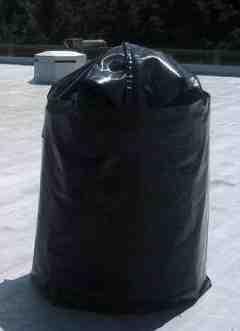
\includegraphics[width=0.30\textwidth,height=0.2\textheight]{images/venezuela/hugo.jpg}
\caption{One of the WCD of the Venezuela LAGO site, called Hugo.}
\label{fig:wcd-ven}
\end{figure}  

Se cuenta con un fotomultiplicador de 5 pulgadas con su divisor de Voltaje,
cuyo diseño fue suministrado por la colaboración LAGO- Perú. Este
fotomultiplicador esta en procesos de pruebas, lo que se ha obetido hasta ahora
es el pulso mostrado en figura 7
  
 \begin{figure}[htp!]
     \centering
     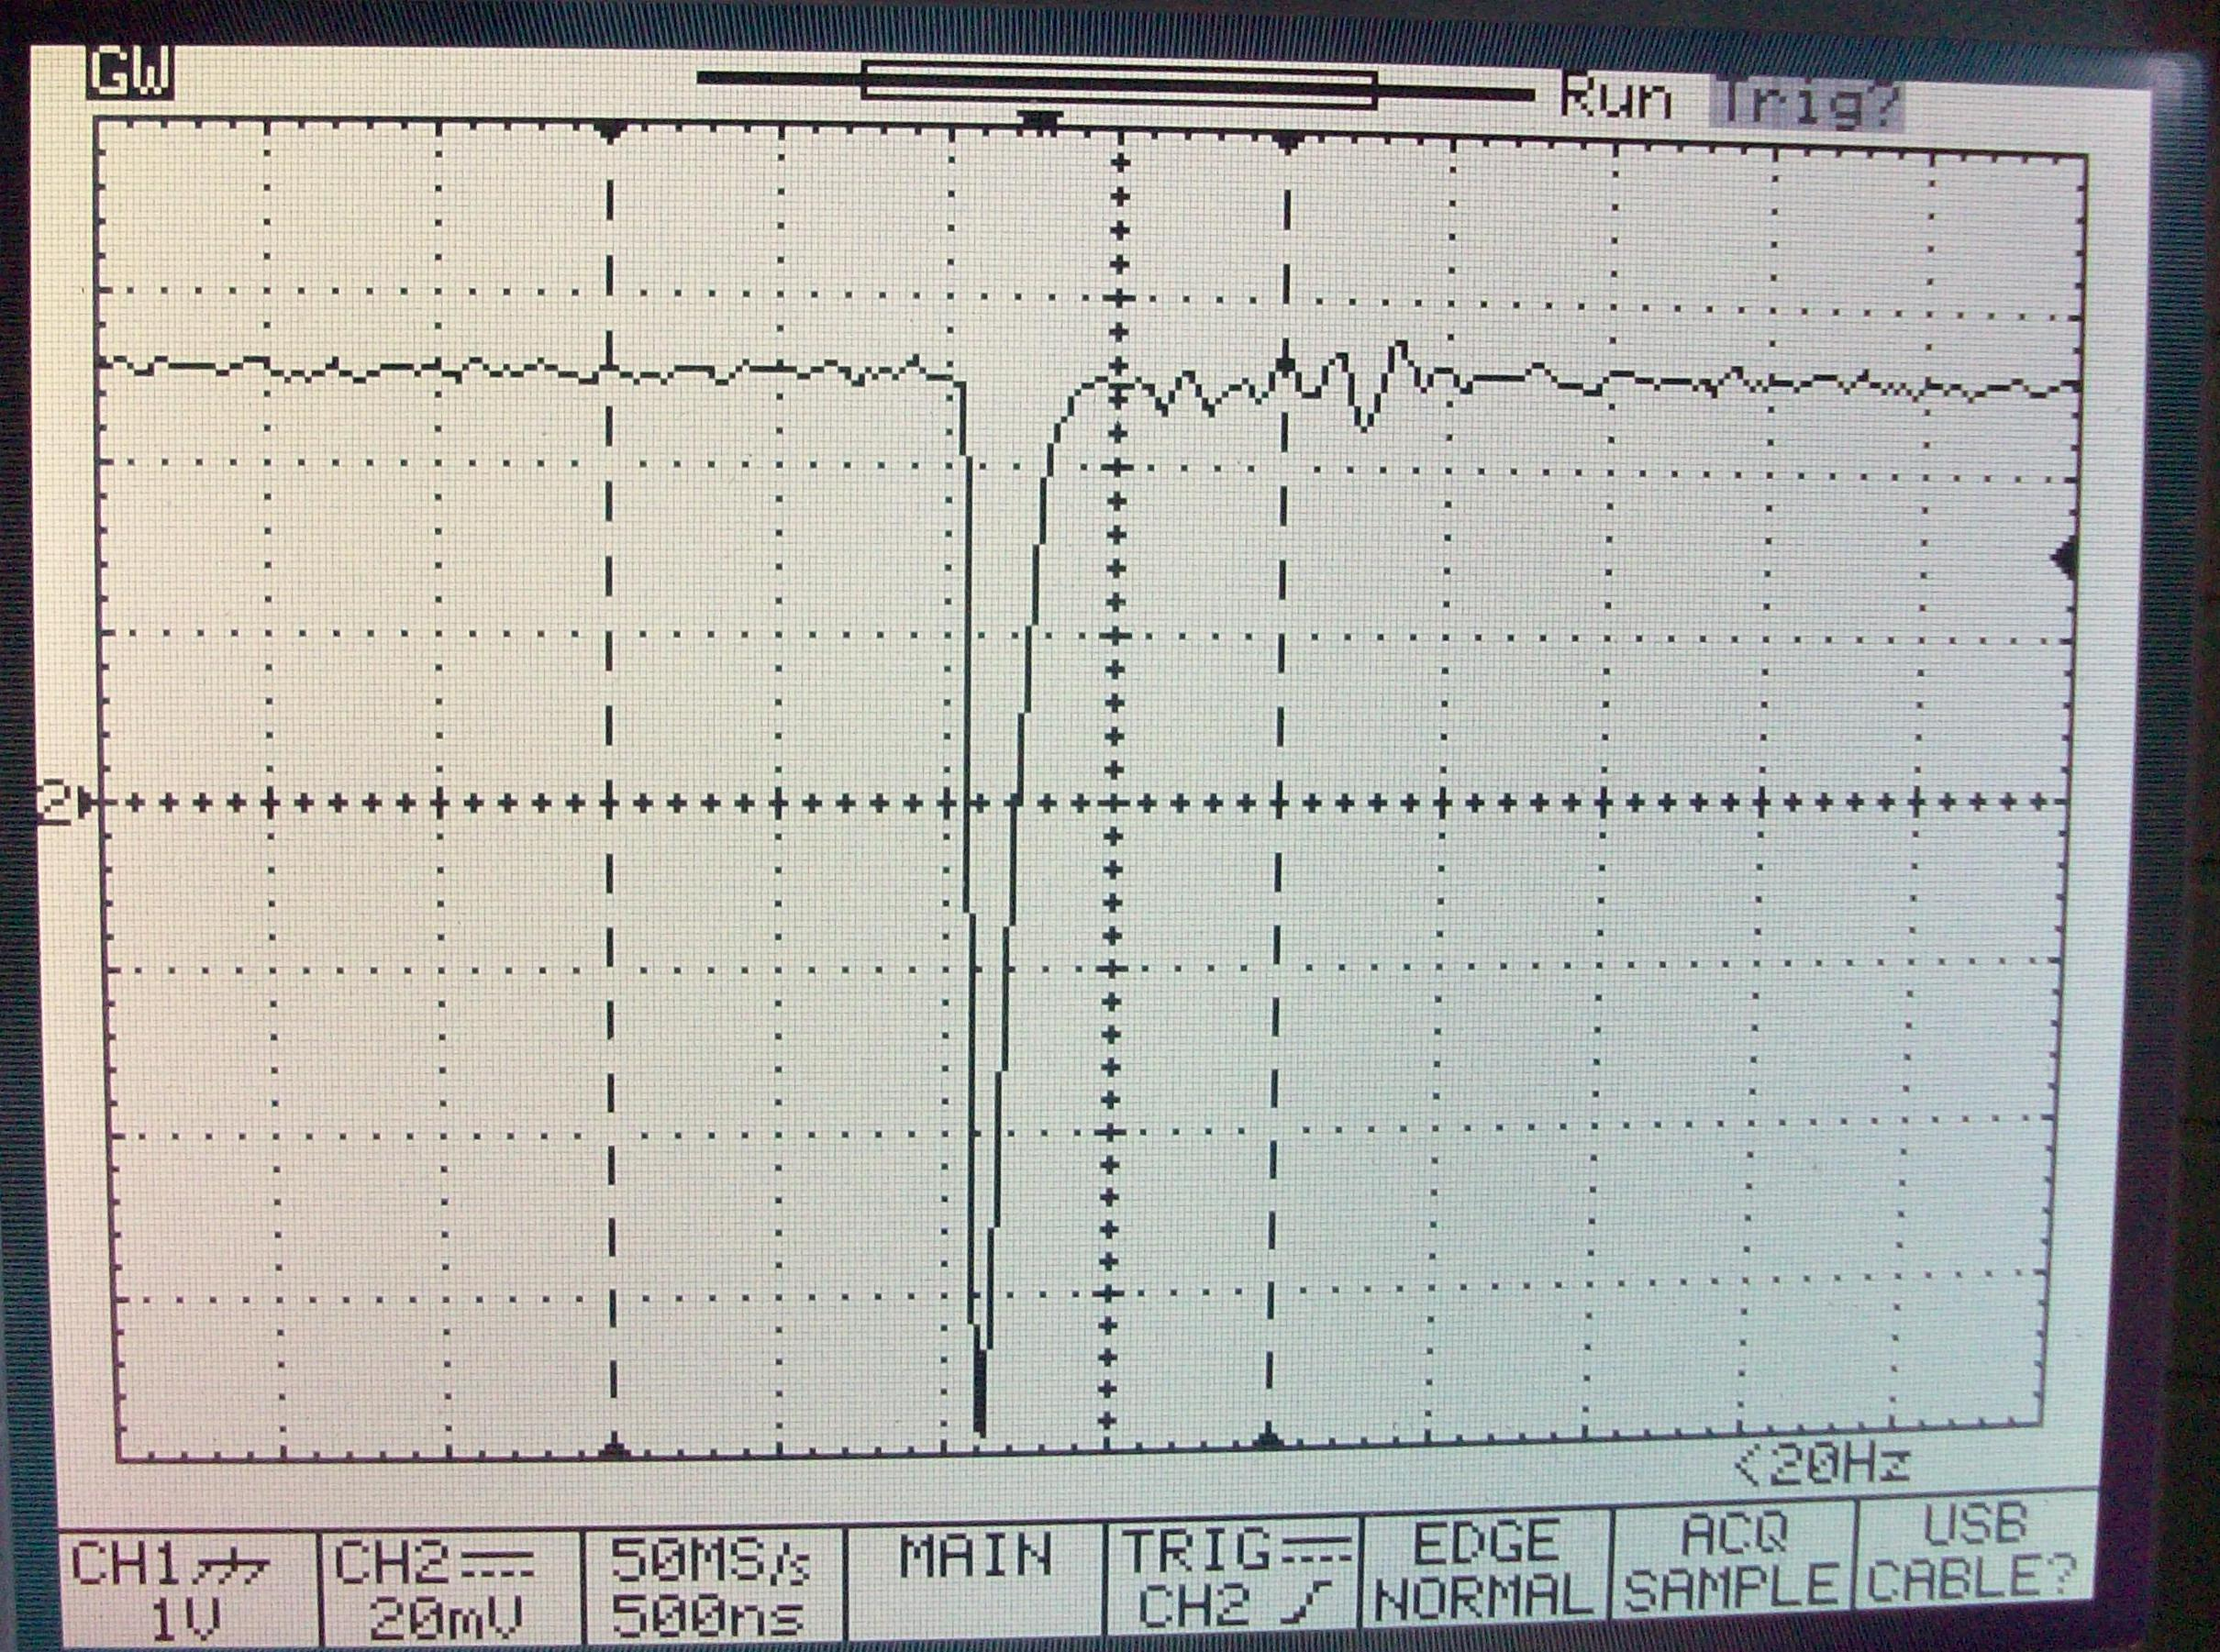
\includegraphics[width=0.65\textwidth,height=0.30\textheight]{images/venezuela/pulsopmt.jpg}
      % nexys2.jpeg: 231x218 pixel, 72dpi, 8.15x7.69 cm, bb=0 0 231 218
     \caption{Pulso con el Fotomultiplicador Pequeño con un Voltaje de $\sim 1800V$} 
     \end{figure}  
 
  
  %9
\section{Data uniformity} \label{sec:data}

LAGO has been developing two main initiatives to deploy a network of curated data repositories:

\begin{enumerate}
  \item to preserve, curate and share the data registered by the large aperture
WCD array, now through a data repository (DR) and in the near future across a
network of DR

 \item to generate a toolkit of scripts and algorithms to detect
the proper operation of the detector. This toolkit will be part of the next
generation of firmware and will allows the system to reconfigure some of its
parameters in order to minimize some of diagnosed malfunctioning.  

 \item to offer a computational infrastructure that allows the collaboration
members to analyze the curated data efficiently

\end{enumerate} 

These initiatives aim to pave the way to openly share the data
recorded with any other domain disciplines.

The reasons for preserving data derive from the fact that observations,
knowledge and understanding are cumulative. Data arise either from measurements
(observational or experimental data), simulated results (synthetic data
computed with mathematical models) or historical records (historical data).
Metadata can facilitate \cite{MichenerEtal1997}:

\begin{itemize}
  \item data identification and acquisition for a given
      subject, for a specific period of time or geographic
      location;
  \item automatic analysis and data modeling;
  \item the inclusion of semantic knowledge elements
      associated with the data.
\end{itemize}


LAGO developed a prototype of  data repository, \texttt{LAGOData}
\cite{TorresEtAl2011} as a part of a more ambitious project,
\texttt{LAGOVirtual}\cite{CamachoEtal2009}, oriented to develop a working
environment to have access and to analyzed the data recorded in all LAGO Sites.
In \texttt{LAGOData}  repository the data are classified  into three types:
instrument calibration data, WCD data sets and simulated data sets. In a near
future this repository will also preserve papers, thesis, Labs Notes and
reports related with the project.

Each data file is tagged by a metadata set specifically adapted to LAGO. The
existence and implementation of a scientific metadata standard model will allow
an uniform access to data for all the members of LAGO colaboration, the
interoperability between scientific information systems and also will
contribute to the data preservation and its usability in time. The metadata
model we propose for \texttt{LAGOData} is an adaptation of the model raised for
the Council for the Central Laboratory of the Research Councils \cite{Sufi2004}

We have developed a prototype of the data repository for the LAGO collaboration
adapting the system  DSpace  \cite{SmithEtal2003}, an open source software that
enables open sharing of many types of content, generally used for institutional
repositories.  Dspace can expose the data and metadata through the Open
Archives Initiatives Protocol for Metadata
Harvesting\footnote{\href{http://www.openarchives.org/OAI/2.0/openarchivesprotocol.htm}{http://www.openarchives.org/OAI/2.0/openarchivesprotocol.htm}}
(\cite{VanSopelEtal2004}) . This protocol is used  by external systems to
collect the data and metadata and create services of agregated value like
meta-searchers. Also offers the data through Really Simple Syndication
channels, RSS, which is available at all levels in the structure of the
repository. These channels are a simple mechanism to show the contents recently
submitted. The detailed description of the implementation of this data
repository based on DSpace can be found in \cite{TorresEtAl2011} and an
interesting survey of a hundred of DR can be found in
\cite{MarcialHemminger2010}.

We expect to release a second version of \texttt{LAGOData} which will have an
implementation of the SWORD ( for \textit{Simple Web-service Offering
Repository Deposit}  ) protocol which became a way to address the need for a
standardised deposit interface to digital repositories
\cite{LewisDeCastroJones2012}. With this implementation  we will be not only
able to synchronize a network of DR across all LAGO site, but also to
automatically stamp a basic metada each data set collected at each WCD of the
LAGO Collaboration.
 
 Additionally, LAGO the electronics is very sensible to atmospheric
electromagnetic disturbances. Typically thunderstorms, that generate severe
change in pressure, temperature  and other weather electric disturbances which
can be associated with antipulses or high variations in voltage. These ghost
signals produced by intense variation on the recording whether variables (or
environmental electric fields) have to be excluded  from curated data sets. To
identify and remove ghost signals on the curated data sets we have performed an
sliding time window analysis looking for signals having 3$\sigma$ deviations
from the average. The sliding window analysis, is an standard strategy where
statistical parameters are calculated for a small frame, or window, of the
data. The window incrementally advances across the surveyed region and, at each
new position, an the new statistical indicators are calculated. In our case, we
have selected $60s$ as a frame window, with a sliding increment of $0.2s$. The
analysis was performed over all data files, from Sierra Negra and Chacaltaya
LAGO sites, that passed the above criterium of the 200 GPS clock marks. We had
found and remove two ghost signals produced by a significant variations of the
electronics baseline. Those data sets that comply with both above criteria (200
clock marks and no ghost signals) are called Good Run List and are available at
the LAGO DR \cite{Sarmiento2012}.

\section{Conclusions}\label{sec:conclusions}

%\newpage % Please avoid layout-changing commands if not strictly necessary
\acknowledgments
Deberiamos poner acknoledgments de todos los paises.


LAGO Colombia gratefully acknowledge for the financial support of the
Vicerrector\'ia de Investigaci\'on y Extensi\'on de la Universidad Industrial
de Santander. The LAGO Collaboration has been benefited from the advanced
computational infrastructure provided by the Centro de Supercomputaci\'on y
C\'alculo Cient\'ifico (SC3) de la Universidad Industrial de Santander. We are
also in debt of the financial support of RedCLARA funding support through the
ALICE2 project and form the International Centre for Theoretical Physics under
the External Office Activities programs.


\bibliography{biblio}
\end{document}
